% Options for packages loaded elsewhere
\PassOptionsToPackage{unicode}{hyperref}
\PassOptionsToPackage{hyphens}{url}
%
\documentclass[
  openany]{book}
\usepackage{amsmath,amssymb}
\usepackage{lmodern}
\usepackage{iftex}
\ifPDFTeX
  \usepackage[T1]{fontenc}
  \usepackage[utf8]{inputenc}
  \usepackage{textcomp} % provide euro and other symbols
\else % if luatex or xetex
  \usepackage{unicode-math}
  \defaultfontfeatures{Scale=MatchLowercase}
  \defaultfontfeatures[\rmfamily]{Ligatures=TeX,Scale=1}
\fi
% Use upquote if available, for straight quotes in verbatim environments
\IfFileExists{upquote.sty}{\usepackage{upquote}}{}
\IfFileExists{microtype.sty}{% use microtype if available
  \usepackage[]{microtype}
  \UseMicrotypeSet[protrusion]{basicmath} % disable protrusion for tt fonts
}{}
\makeatletter
\@ifundefined{KOMAClassName}{% if non-KOMA class
  \IfFileExists{parskip.sty}{%
    \usepackage{parskip}
  }{% else
    \setlength{\parindent}{0pt}
    \setlength{\parskip}{6pt plus 2pt minus 1pt}}
}{% if KOMA class
  \KOMAoptions{parskip=half}}
\makeatother
\usepackage{xcolor}
\usepackage{graphicx}
\makeatletter
\def\maxwidth{\ifdim\Gin@nat@width>\linewidth\linewidth\else\Gin@nat@width\fi}
\def\maxheight{\ifdim\Gin@nat@height>\textheight\textheight\else\Gin@nat@height\fi}
\makeatother
% Scale images if necessary, so that they will not overflow the page
% margins by default, and it is still possible to overwrite the defaults
% using explicit options in \includegraphics[width, height, ...]{}
\setkeys{Gin}{width=\maxwidth,height=\maxheight,keepaspectratio}
% Set default figure placement to htbp
\makeatletter
\def\fps@figure{htbp}
\makeatother
\setlength{\emergencystretch}{3em} % prevent overfull lines
\providecommand{\tightlist}{%
  \setlength{\itemsep}{0pt}\setlength{\parskip}{0pt}}
\setcounter{secnumdepth}{-\maxdimen} % remove section numbering
\newlength{\cslhangindent}
\setlength{\cslhangindent}{1.5em}
\newlength{\csllabelwidth}
\setlength{\csllabelwidth}{3em}
\newlength{\cslentryspacingunit} % times entry-spacing
\setlength{\cslentryspacingunit}{\parskip}
\newenvironment{CSLReferences}[2] % #1 hanging-ident, #2 entry spacing
 {% don't indent paragraphs
  \setlength{\parindent}{0pt}
  % turn on hanging indent if param 1 is 1
  \ifodd #1
  \let\oldpar\par
  \def\par{\hangindent=\cslhangindent\oldpar}
  \fi
  % set entry spacing
  \setlength{\parskip}{#2\cslentryspacingunit}
 }%
 {}
\usepackage{calc}
\newcommand{\CSLBlock}[1]{#1\hfill\break}
\newcommand{\CSLLeftMargin}[1]{\parbox[t]{\csllabelwidth}{#1}}
\newcommand{\CSLRightInline}[1]{\parbox[t]{\linewidth - \csllabelwidth}{#1}\break}
\newcommand{\CSLIndent}[1]{\hspace{\cslhangindent}#1}
\ifLuaTeX
\usepackage[bidi=basic]{babel}
\else
\usepackage[bidi=default]{babel}
\fi
\babelprovide[main,import]{english}
% get rid of language-specific shorthands (see #6817):
\let\LanguageShortHands\languageshorthands
\def\languageshorthands#1{}
\usepackage[fontsize=12pt]{scrextend}
\usepackage{titling}
\pretitle{\begin{center}\vspace{5cm}\LARGE}
\posttitle{\end{center}}
\preauthor{\begin{center}\vspace{1.5cm}\Large\textit}
\postauthor{\end{center}}
\predate{\begin{center}\vspace{1cm}\Large\textit}
\usepackage{booktabs}
\usepackage{longtable}
\usepackage{array}
\usepackage{multirow}
\usepackage{wrapfig}
\usepackage{float}
\usepackage{colortbl}
\usepackage{pdflscape}
\usepackage{tabu}
\usepackage{threeparttable}
\usepackage{threeparttablex}
\usepackage[normalem]{ulem}
\usepackage{makecell}
\usepackage{xcolor}
\ifLuaTeX
  \usepackage{selnolig}  % disable illegal ligatures
\fi
\IfFileExists{bookmark.sty}{\usepackage{bookmark}}{\usepackage{hyperref}}
\IfFileExists{xurl.sty}{\usepackage{xurl}}{} % add URL line breaks if available
\urlstyle{same} % disable monospaced font for URLs
\hypersetup{
  pdftitle={Harvested Wood Products Carbon Model, Version R Documentation},
  pdflang={en},
  hidelinks,
  pdfcreator={LaTeX via pandoc}}

\title{Harvested Wood Products Carbon Model, Version R Documentation}
\author{Jeremy Groom, Ph.D.\\
Groom Analytics, LLC\\
\strut \\
Nadia Tase\\
California Department of Forestry and Fire Protection}
\date{Date: October 04, 2022}

\begin{document}
\frontmatter
\maketitle

\mainmatter
\hypertarget{sum}{%
\chapter{Summary}\label{sum}}

The Harvested Wood Products (HWP) model calculates cumulative HWP carbon
stocks and emissions using the
\href{https://www.ipcc-nggip.iges.or.jp/public/2006gl/pdf/4_Volume4/V4_04_Ch4_Forest_Land.pdf}{Tier
3 Production Approach} carbon estimation guidelines developed by the
\href{https://www.ipcc.ch/}{Intergovernmental Panel on Climate Change}.
It is a deterministic model which relies on optional and required
user-supplied information. The model estimation methods are described in
Stockmann et al. (\protect\hyperlink{ref-stockmann2012}{2012}). There
have been several builds of the model, originally created by the U.S.
Forest Service (USFS), on platforms including Microsoft Excel and C++.
Through partnership with the California Department of Forestry and Fire
Protection (CAL FIRE), Oregon Department of Forestry (ODF) and Groom
Analytics LLC, this version of the tool (deemed HWP-C vR) builds from
the previous USFS versions on the R (\protect\hyperlink{ref-R-base}{R
Core Team 2021}) platform, for use in their state-level harvested wood
product carbon inventories. Another USFS effort is currently underway to
construct an interactive version of the model in Python. This version
(HWP-C vR) is not intended to compete with or contradict the original or
ongoing USFS work, but rather complement the work by being available in
a different platform and coding language. This version also includes new
data visualizations.

Here we describe the HWP-C vR build of the model based on data from the
U.S. west coast states of California, Oregon, and Washington. Users may
explore California and Oregon data via the
\href{https://groomanalyticsllc.shinyapps.io/HWP-C-vR/}{R Shiny web
application}. Users from any state or ownership may also upload their
own data onto the app, run their data through the HWP model and
associated Monte Carlo simulation, view and interact with figures, and
download figures and tables.

Alternatively, users may access the full Shiny app R code as well as a
stand-alone version of the R code for HWP model implementation. The
stand-alone version allows users the opportunity to step through the
code more easily, save intermediate outputs (i.e., arrays) for
hand-calculation of outcomes, and alter the code to meet their own data
needs. Both versions allow users to download or generate the final
output tables necessary to recreate figures to their own specifications.

This document describes the model and structure of the code, explains
how to generate input files, and provides instruction on accessing the
code.

\hypertarget{sum-ack}{%
\section{Acknowledgements}\label{sum-ack}}

Many thanks to Nadia Tase (California Department of Forestry and Fire
Protection - CAL FIRE) and Andrew Yost (Oregon Department of Forestry -
ODF) for supporting the development of this work through feedback,
discussion, and their own efforts to dive into the code and understand
the model at its core. Jimmy Kagan (Oregon State University's Institute
for Natural Resources) and Amanda Reynolds (CAL FIRE) provided
administrative support. This work would not be possible without the
original work completed by Nate Anderson (United States Forest Service -
USFS), Keith Stockmann (USFS), Dan Loeffler (University of Montana), and
others. The information and feedback they shared has been invaluable.
Feedback and support for an earlier iteration of the R-version of the
model from Todd Morgan (University of Montana, Bureau of Business and
Economic Research) has also been indespensible.

This project was funded by the California Department of Forestry and
Fire Protection Purchase Order 3540-0000277546. Earlier work on the
project was funded by the Oregon Department of Forestry and supported by
the Institute for Natural Resources, Oregon State University.

\hypertarget{sum-abb}{%
\section{Abbreviations}\label{sum-abb}}

The following description uses many acronyms for brevity. Here is a list
of the most common:

BBF: Billion Board Feet\\
BF: Board Feet\\
BLM: Bureau of Land Management\\
CCF: Hundred Cubic Feet\\
CF: Cubic Feet\\
DEC: Discard Energy Capture\\
EEC: Emitted with Energy Capture\\
EUR: End-use Product Ratios\\
EWOEC: Emitted without Energy Capture\\
HWP: Harvested Wood Products\\
IPCC: Intergovernmental Panel on Climate Change\\
MBF: Thousand Board Feet)\\
MMT C: Million Metric Tons of Carbon\\
MT: Metric Tons\\
PIU; Products in Use\\
PPR: Primary Product Ratios\\
SWDS: Solid Waste Disposal Sites\\
Tg C: Teragrams of Carbon: Tg C\\
Tg CO2e: Teragrams of Carbon Dioxide Equivalent\\
TPO: Timber Product Output\\
TPR: Timber Product Ratios\\
USFS: United States Forest Service

A note about units for carbon:\\
Publications from the United States have frequently described carbon
storage and emissions using the metric million metric tons carbon, or
MMT C. We are using the equivalent metric, teragrams of carbon (Tg C) in
the HWP model and this manual to align with common scientific reporting
units. Additionally, though the tool provides estimates for carbon
emissions in both units of carbon and carbon dioxide equivalents, these
estimates are for the biogenic carbon content in the wood only, and do
not include other carbon-based greenhouse gas emissions with different
global warming potentials, such as methane.

\hypertarget{int}{%
\chapter{Introduction}\label{int}}

\hypertarget{int-struc}{%
\section{Structure of this document}\label{int-struc}}

We wish to provide users with a document that will enable users to step
into the HWP-C vR model to the degree that they find comfortable and
useful. This could range from manipulating pre-loaded California and
Oregon data from the web app to downloading all of the code onto their
machine and modifying it to their purposes. We laid out the sections to
reflect this progression.

\begin{itemize}
\tightlist
\item
  Chapter @ref(sum): This section provides a brief overview of the
  model, a list of abbreviations, an explanation of units used, and
  acknowledgements.\\
\item
  This chapter (Chapter @ref(int)): Here we provide some background on
  the model including a bit of history and a description of how it
  functions. We also discuss some of the model's assumptions and future
  work.
\end{itemize}

The next three sections describe options for interacting with the model
in progressively technical ways:

\begin{itemize}
\tightlist
\item
  Option 1: Chapter @ref(app). Basic - Users can explore and view
  pre-laoded HWP C data in the R Shiny web application.

  \begin{itemize}
  \tightlist
  \item
    Users can view a, interact with, and download a variety of graphical
    outputs from the California and Oregon default data sets and
    manipulate the figures to a degree.
  \item
    Outputs that can be viewed in or downloaded from the web application
    are described in section 5.7.\\
  \end{itemize}
\item
  Option 2: Chapter @ref(own). Intermediate - Users can provide their
  own data to run in the R Shiny web application to generate HWP C
  estimates.

  \begin{itemize}
  \tightlist
  \item
    Users can use the full functionality of the app on their own data,
    including generating HWP carbon storage and emissions estimates,
    producing, viewing, and downloading the same sorts of figures, and
    runing the Monte Carlo uncertainty analysis.\\
  \item
    This is a good option for users that would like to produce their own
    results but are unfamiliar with R or R Studio.
  \end{itemize}
\item
  Option 3: Chapter @ref(dnld). Advanced - Users can download the Shiny
  web application and R code to run the model on to their own computer.

  \begin{itemize}
  \tightlist
  \item
    Allows the user to run the Shiny web app locally on their own
    machine.\\
  \item
    Also allows the user to operate the stand-alone version of the model
    using the R code in R or R Studio without needing to rely on the web
    app.
  \item
    Users can use existing datasets for California, Oregon, and
    Washington or provide their own input datasets to generate
    cumulative estimates of harvested wood product carbon storage and
    emissions.
  \end{itemize}
\end{itemize}

Chapter @ref(model) describes in detail the operation of the HWP-C vR
model as well as the Monte Carlo simulation. Chapter @ref(ft) contains
frequently asked questions and troubleshooting advice. Following Chapter
@ref(ft) is the bibliography. Although each HTML chapter contains a
bibliography, the PDF version only has this final bibliography section.

\hypertarget{int-purp}{%
\section{General purpose and utility of the HWP C
model}\label{int-purp}}

The HWP C model was originally created for U.S. Forest Service (USFS)
National Forest System Regional HWP carbon inventories, and later
modified for state-level inventories in California, Oregon and
Washington. The history of this model is described in more detail in
Section @ref(int-hist). The current iteration of this model supports
state-level carbon inventories but could be used by any jurisdiction or
landowner.

This HWP C model (and associated visualizations) is a long-term
accounting tool for carbon emissions and storage from harvested wood
products. Users can easily understand how harvest levels have changed
over time, by ownership and in total. Given changes in disposal methods
and the assumed lifetime use of wood products, users can examine what
proportion of harvested wood products remain in use, in disposal sites,
or as biogenic carbon emitted to the atmosphere.

The model may also be useful for planners and decision-makers to explore
hypothetical wood utilization scenarios and understand the long-term
storage and emissions consequences of differing harvest levels or
promoting wood products with different use lifespans.

\hypertarget{int-gen}{%
\section{General description of the HWP C model}\label{int-gen}}

An overview schematic of the HWP model is provided in Figure
@ref(fig:overview-fig). The model estimates cumulative HWP carbon stocks
and emissions from current and historic harvests using the
\href{https://www.ipcc-nggip.iges.or.jp/public/2006gl/pdf/4_Volume4/V4_04_Ch4_Forest_Land.pdf}{Tier
3 Production Approach} carbon estimation guidelines developed by the
\href{https://www.ipcc.ch/}{Intergovernmental Panel on Climate Change}.
For each year of consideration, the model allocates annual harvest
volumes in thousand board feet (MBF) to timber products (e.g., sawlogs,
non-sawtimber, pulpwood, fuelwood, etc.) and primary products (e.g.,
lumber, plywood, panels, pulp, etc.) using timber product ratios (TPR)
and primary product ratios (PPR). Total harvest volumes or volumes
partitioned by ownership can be analyzed. Conversion factors are used to
convert harvest volumes in thousand board feet (MBF) to cubic foot (CF)
volumes. Primary product volumes in cubic feet are then converted to
units of carbon using conversions from Smith et al.
(\protect\hyperlink{ref-smith2006}{2006}). Primary products are then
distributed to end-uses using ratios (EUR) from McKeever
(\protect\hyperlink{ref-mckeever2009}{2009}) and McKeever and Howard
(\protect\hyperlink{ref-mckeever2011}{2011}), such as lumber in single
family homes versus lumber in packaging and shipping materials. The
carbon associated with primary products in each end-use comprises the
``products in use'' (PIU pool) HWP carbon pool. Approximately 8\% of the
carbon immediately enters discard pathways to reflect a loss factor when
primary products enter the PIU pool. Each end-use has a different
functional lifespan, or half-life, which determines the amount and rate
at which harvested wood products are retired from the PIU pool to
various discard pathways each year.

Retired HWPs are transferred to a solid waste disposal site (SWDS),
recycled, composted, or burned with or without energy capture using
discard disposition ratios. Discard emissions pathways with immediate
oxidation include discarded products that are burned (with or without
energy capture) or composted. Discard storage pathways include products
that are recycled (products re-enter the in-use pool) or disposed into
landfills and dumps, which comprise the SWDS pool. The landfill fixed
carbon ratio determines the portion of carbon that remains permanently
inert in the anaerobic environment of landfills. Decay half-lives are
applied to carbon in dumps and the decaying portion in landfills of the
SWDS pool to determine the quantity and rate at which carbon is emitted
from this pool. All data sources for harvest volumes, timber and primary
product ratios, board foot to cubic foot volume conversions, primary
product volume to carbon conversions, loss factors, the distribution of
HWPs to end-uses, the functional life span of wood products,
distribution of HWPs to the various disposal pathways, landfill fixed
carbon ratios and decay half-lives are provided in the individual
state-level reports (e.g., Loeffler et al.
(\protect\hyperlink{ref-loeffler2019}{2019}), Morgan et al.
(\protect\hyperlink{ref-morgan2021}{2021}), Nichols et al.
(\protect\hyperlink{ref-nichols2020}{2020})), and are also described in
Section @ref(own-prov-input).

With each year of harvest more carbon enters the cycle. Some carbon is
immediately oxidized as fuelwood, enters the products in use pool, or is
discarded immediately. However, some carbon from the previous harvest
year can remain stored as carbon in products in use, dumps, landfills,
or recovered products, while some is emitted through decay from dumps,
the decaying portion of landfills, compost, or waste incineration. The
model provides cumulative carbon storage and emissions for all harvest
years analyzed. All carbon emission estimates from this model are for
the biogenic carbon content of the harvested wood only and do not
include emissions in the form of other carbon-containing greenhouse
gasses such as methane. Intermediate outputs (i.e., arrays) and some
figures allow users to explore outputs from single harvest years.

Lastly, the model provides a Monte Carlo analysis of uncertainty in the
estimates for carbon stored in both the PIU and SWDS pools and both
pools combined, as well as carbon emitted with or without energy
capture.

\begin{figure}
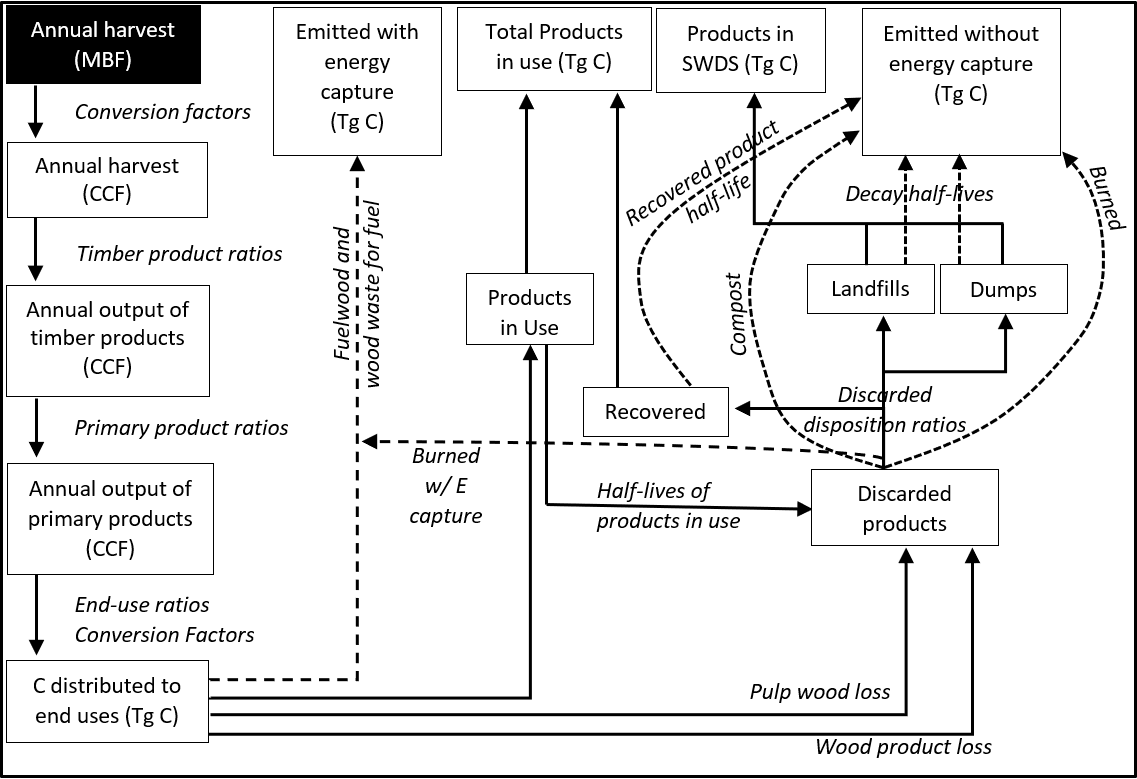
\includegraphics[width=1\linewidth]{images/OverviewModelSchematic} \caption{General schematic for calculations to quantify HWP storage and emissions, based on Figure 7 in Stockmann et al. 2012.  Note that in this version Compost is not connected to SWDS, an arrow to SWDS has been added for emissions from Recovered, and that the code calculates end-use C distribution in one step after organizing TPO, PPR, EUR, and conversion factors.}\label{fig:overview-fig}
\end{figure}

\hypertarget{int-assump}{%
\section{HWP model assumptions}\label{int-assump}}

The HWP model follows the IPCC Production Approach for carbon
estimation; therefore, HWPs exported from the area of analysis are
included but imported HWPs are excluded. In this way, the model is
closed and tracks only carbon harvested within a specified area.
Therefore, at a state level, carbon storage in and emissions from HWP
consumed within the state boundaries may be greater than expected from
timber harvested within the state if the state imports timber or timber
products. Currently, the model assumes timber or timber products
exported to other jurisdictions or countries experience the same
utilization parameters, disposal rates and pathways, and decay processes
as those of the area of analysis. For example, California-origin harvest
that is exported is subject to California parameters. If exported wood
experiences different utilization parameters, disposal rates and
pathways, or decay processes, results could be erroneous. The potential
magnitude of errors depends on both the overall quantity exported as
well as the magnitude of differences in the parameters.

The model relies on many different data types. The model assumes that
all underlying datasets, such as harvested timber volume and ratios such
as timber product ratios (TPR), primary product ratios (PPR), end-use
product ratios (EUR), discard ratios, end-use product half-lives, and
decay rates are valid. Citations for all datasets are provided; however,
there is inherently some level of uncertainty in the precision or
accuracy of the datasets as they rely on a number of other analyses,
datasets, are in areas of active research, are provided at national or
international scales rather than local or regional, or have not been
updated recently. Sections @ref(own-prov-input-harvest) --
@ref(own-prov-input-discHL) describe in more detail the scale and
sources of these datasets and when they were last updated. The model
results can be expected to be precise or accurate to the extent the
underlying datasets are precise and accurate.

The model also provides certain pathways, such as for recycling or
disposal to landfills. These pathways are assumed to adequately
represent reality. In the model, recycling is represented through a
simplified process where a portion of PIU are recycled once and then
subject to a single, very short half-life. In reality, products may be
recycled multiple times into potentially long-lived uses. The
representation of recycling in this model may result in an
underestimation of the amount of recycling and continued storage of
carbon in PIU that occurs and an overestimation of recycled products
emissions. Similarly, PIU disposed to landfills enter a generic landfill
pool with a single landfill decay rate, whereas in reality there are
many types of landfills with varying landfill decay rates. Additionally,
when primary products enter the PIU pool, the loss factor is currently
only applied to solid wood products. However, literature supports a loss
factor for paper as well (\protect\hyperlink{ref-skog1998}{Skog and
Nicholson 1998}). Though paper is already a short lived product, this
may result in an overestimation of emissions earlier than they might
otherwise occur in reality. Several other pathways and processes in the
model exist that have an unknown set of implications depending on how
closely they mimic reality. For example, the model represents decay
through a first order decay function while other decay functions may be
more appropriate. The model also omits certain pathways that may result
in additional carbon storage and emissions associated with harvested
wood. For example, in some jurisdictions substantial bark utilization
occurs. While bark is not considered a harvested wood product from an
IPCC roundwood source (\protect\hyperlink{ref-buendia2019}{Buendia et
al. 2019}) and is rather considered a byproduct, utilization of this
material typically results in additional fuelwood emissions. IPCC
(\protect\hyperlink{ref-ipcc2014}{2014}) recognizes that there are other
sources of feedstock for commodities besides industrial roundwood or
wood pulp and encourages countries to use country-specific data. In this
way, it may be important for states like California where bark is
utilized for energy production
(\protect\hyperlink{ref-marcille2020}{Marcille et al. 2020}) to consider
additional measures to account for bark utilization. It is a goal to add
functionality to estimate carbon storage and emissions associated with
bark utilization to subsequent versions of this model.

The Monte Carlo analysis attempts to explore the range of possible
outcomes given different levels of certainty in the data. There are
potential limitations to the Monte Carlo analysis itself. As the degree
of uncertainty has not currently been quantified for most datasets,
uncertainty parameters have been provided for each variable based on
expert opinion. Additionally, the Monte Carlo analysis takes a specific
approach towards varying the ratios, constraining all ratios to sum to
one. Given the selected range of possible values for each variable, the
resulting randomly selected values may not be independent from one
another and may be unintentionally biased. That is, within a ratio type
that must sum to one and for a particular model iteration, if one value
is randomly selected to equal 1.0, the remaining values for that ratio
set must equal 0 (see Section @ref(model-mc-res)). Lastly, the Monte
Carlo analysis does not include a parameter for the accuracy of the
processes and pathways represented in the model as a whole, for example,
how recycling, or landfill disposal, or decay is represented.

Currently, the model does not estimate emissions for other carbon-based
greenhouse gases. For example, it does not differentiate between carbon
in landfills that is emitted as methane vs.~CO\(_2\). Methane is a much
more potent greenhouse gas than CO\(_2\), albeit with a shorter
residence time. Consequently, greenhouse emissions associated with HWPs
are likely much higher than the estimates based only on the
carbon-content of wood provided by this model. Though landfill methane
emissions would be accounted in the IPCC Waste sector, this information
is still valuable for determining the potential climate benefits,
impacts and mitigation opportunities associated with HWPs.

For a full discussion on the underlying data sets, sources, represented
HWP pathways and processes, and potential limitations, and implications,
please refer to Lucey et al. (\protect\hyperlink{ref-lucey202X}{In
review}).

Finally, this model does not include any method for overall model
validation. Estimates for individual, underlying datasets feeding into
the model, or certain pathways and processes can still be improved. But,
like all models, the HWP model simplifies reality and hopefully provides
users with useful insight by tracking and summarizing complicated
calculation outputs in a reasonable way.

\hypertarget{int-hist}{%
\section{Model history}\label{int-hist}}

The HWP model began as an Excel macro originally created by the U.S.
Forest Service (USFS) to estimate an HWP carbon inventory for the
Northern Region of the National Forest System
(\protect\hyperlink{ref-stockmann2012}{Stockmann et al. 2012};
\protect\hyperlink{ref-anderson2013}{Anderson et al. 2013}). The Excel
version was updated to one programmed in C++ for the remaining USFS
Regional HWP carbon inventories (USFS HWP-C; e.g., Butler, Stockmann,
Anderson, Skog, et al. (\protect\hyperlink{ref-butler2014nw}{2014}),
Loeffler et al. (\protect\hyperlink{ref-loeffler2014sr}{2014b}),
Stockmann et al. (\protect\hyperlink{ref-stockmann2014imr}{2014c})). The
model was then modified in 2017 by the USFS for use in the California
Forest Ecosystem and Harvested Wood Product Carbon Inventory
(\protect\hyperlink{ref-loeffler2019}{Loeffler et al. 2019}) and is
given the label here as the CA USFS HWP-C variant. This history is
depicted in Figure @ref(fig:hist-fig). Though names for the USFS
versions of the model did not exist, they are given here for clarifying
purposes. However, in 2020 when Oregon and California were trying to
establish or update HWP C inventories, no version of the HWP C model was
available publicly, as the USFS's hosting partner's server expired and
older coding languages used in previous iterations of the model were no
longer operational and being updated.

Building from the previous USFS-led versions of the model, Groom
Analytics LLC undertook programming the model in R for the Oregon
Department of Forestry (ODF) and California Department of Forestry and
Fire Protection (CAL FIRE), and subsequently deployed the R version as a
\href{https://groomanalyticsllc.shinyapps.io/HWP-C-vR/}{web
application}. This version of the model (HWP-C vR) described in this
document largely functions the same as the original USFS Excel-based
model and the v1 tool. A few changes exist and are described more fully
in Christensen et al. (\protect\hyperlink{ref-christensen2020}{2020},
\protect\hyperlink{ref-christensen2021}{2021}). These changes include:

\begin{itemize}
\tightlist
\item
  Modification of lag times built in the original tool, in order to
  allow users to more easily verify calculations.\\
\item
  The CA USFS HWP-C variant of the tool used for the state-level
  inventory in California was not coded correctly to perform the
  uncertainty analysis. This tool has established a new Monte Carlo
  simulation that has succeeded in introducing variability into the HWP
  C estimates.
\end{itemize}

The USFS is currently updating their original tool, including the
improvements made in the CA USFS HWP-C variant, with public availability
expected in 2022/2023. This version (HWP-C vR) is not intended to
compete with or contradict the original or ongoing USFS work, but rather
complement the original work by being available in a different platform
and coding language. This version also includes new data visualizations.

\begin{figure}
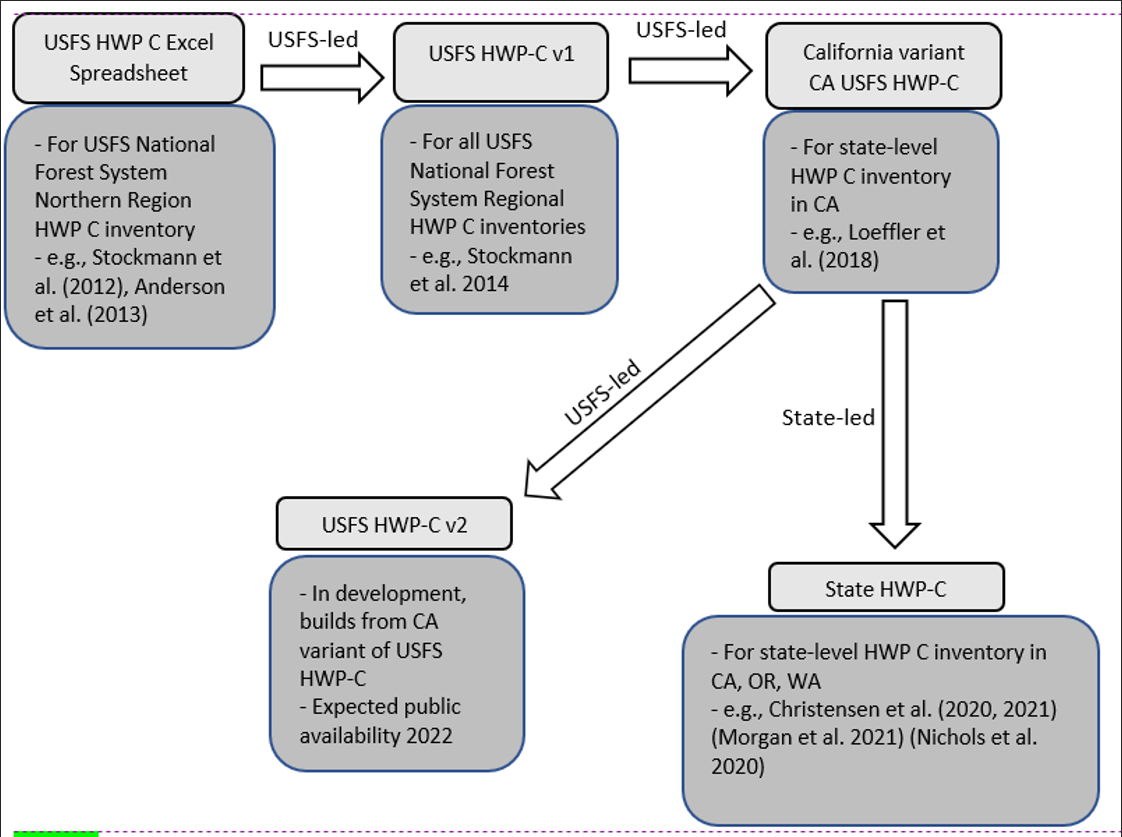
\includegraphics[width=1\linewidth]{images/ModelHistory} \caption{Schematic of the HWP model development pathway.  The version described here is the state-led HWP-C vR variant.}\label{fig:hist-fig}
\end{figure}

\hypertarget{int-future}{%
\section{Future work}\label{int-future}}

HWP carbon estimation is an area of active research. Efforts currently
underway to improve the functionality of this model include adding new
data visualizations and improving upon existing ones. Efforts to provide
a module to estimate carbon storage and emissions associated with bark
utilization is also being explored.

Other directly related research underway at the University of
Massachusetts explores the representation of landfill disposal pathways
in the model, estimation of landfill methane emissions, improvements to
the recycling pathway, and improvements to disposal parameters
specifically for California, with the hope of expanding these
improvements more generally in the model.

Users can improve the model's utility by researching and altering model
input datasets with their own regional information. Updates and
improvements to underlying international, national and regional or local
datasets should be explored.

\hypertarget{app}{%
\chapter{Option 1: Basic use of the R Shiny web application}\label{app}}

\hypertarget{app-sum}{%
\section{Interacting with the HWP-C vR model}\label{app-sum}}

There are two approaches available to users for interacting with the HWP
model. The first way is to use the web application. Users can view a
variety of graphical outputs from the California and Oregon data sets
and manipulate the figures to a degree (this chapter). Users can also
upload their own data (Chapter @ref(own)), run the HWP-C vR model, and
view the results using the same suite of figures. Users can also
download the model to their computer (Chapter @ref(dnld)). This option
allows them to run the web app locally on their own machine. It also
lets them operate a stand-alone version of the model, which is a
code-based environment that does not produce the web app.

\hypertarget{app-shiny}{%
\section{Basic web interactivity -- Shiny app}\label{app-shiny}}

The \href{https://groomanalyticsllc.shinyapps.io/HWP-C-vR/}{web site}
allows users to switch between two pre-loaded data sets, California and
Oregon state-wide timber harvests. The menu bar on the left also has
some drop-down plotting and data upload options. Plots include displays
of \textbf{timber harvest summaries}, \textbf{harvested wood product
carbon storage and emissions estimates}, and \textbf{Monte Carlo
simulation} results.

The app was designed to aid users by providing figures that could
usefully be incorporated into reports. To that end, all figures can be
saved (with one exception) and the title for each figure can be
customized.

Below we describe the figures and options within each menu category

\hypertarget{app-shiny-home}{%
\subsection{Homepage}\label{app-shiny-home}}

The only figure for the app homepage (\textbf{Home}) is an original
drawing by Dr.~Groom's child, Farren Groom. This page offers a brief
overview of the web app.

\hypertarget{app-shiny-timber}{%
\subsection{Timber harvest summary figures}\label{app-shiny-timber}}

The three figure options under Timber Harvest Summaries are
\textbf{Annual Timber Harvest}, \textbf{Fate of Harvest Carbon}, and
\textbf{Harvest by Functional Lifespan}.

\begin{itemize}
\item
  \textbf{Annual Timber Harvest} shows the volume of harvest by year and
  ownership. Users can toggle between seeing annual or cumulative
  versions of total harvest volumes, ownership volumes, or both
  simultaneously. As in all figures, users can select seeing results by
  Tg C or Tg CO\(_2\)e. This figure additionally allows users to see
  results by BBF. Results can be displayed by the year or cumulatively
  over time.
\item
  \textbf{Fate of Harvest Carbon}. This tab has two figures, a Sankey
  diagram and a more static figure to the lower right. The Sankey
  diagram depicts the fate, over time, of harvested carbon from a single
  year. In the bottom left portion of the screen, the user selects the
  harvest date of interest and the years post-harvest to track the fate
  of carbon in the system. Users can, by mouse, manipulate the location
  of the vertical bars associated with the fate of the harvested carbon.
  Mouse-overs of the diagram will also reveal the amount of carbon (Tg C
  / Tg CO\(_2\)e) in pools or transitioning to pools. The same data are
  displayed in the lower-right figure, with the figure displaying over
  time the residence of carbon in different pools and emissions
  categories. The vertical line depicts the data slice displayed in the
  Sankey diagram. The Sankey diagram's html code can be downloaded but
  cannot be saved as a pdf (the stand-alone version of the model can
  provide a PNG-savable version). The lower-right figure may be saved as
  a PNG file.
\item
  \textbf{Harvest by Functional Lifespan}. The HWP model has different
  half-lives for products in use. This figure bins the annual volume of
  harvest sent to different end use products by their associated
  half-lives. Half-life groupings for ``short,'' ``medium,'' and
  ``long'' lifespan categories were determined through expert opinion in
  the Canadian Forest Service, the British Columbia Ministry of Forests,
  the California Department of Forestry and Fire Protection, the Oregon
  Department of Forestry, and the University of Montana Bureau of
  Business and Economic Research. The figure displays values by either
  the harvest volume or proportion of total harvest.
\end{itemize}

\hypertarget{app-shiny-cse}{%
\subsection{Carbon Storage and Emissions figures}\label{app-shiny-cse}}

These four figures, under the Carbon Storage and Emissions menu option,
track the size of pools and emissions categories in Tg C or Tg CO\(_2\)e
over time.

\begin{itemize}
\item
  \textbf{Carbon Storage by Ownership}. If harvest data by ownership are
  available, the figure plots the amount of carbon stored in products in
  use and SWDS. Users can select which ownership values are displayed
  along with whether to display products in use data, SWDS data, or
  both.\\
\item
  \textbf{Carbon Storage and Emissions}. This selection allows viewers
  to access three similar figures of cumulative carbon states over time.
  All three allow users to view any combination of products in use,
  SWDS, and emissions categories.

  \begin{itemize}
  \tightlist
  \item
    Summary Pool and Emission Categories: This figure displays general
    storage (products in use, SWDS) and emissions (emissions with energy
    capture, emission without energy capture).
  \item
    Pool and emission category components: This figure allows users to
    visualize emissions (eg., fuelwood, landfill decay, etc.) and
    storage (e.g., products in use, landfill stock subject to decay,
    etc.) pool components.
  \item
    Pools and emissions by halflife category: Storage and emissions
    categories are displayed by the contribution of immediate oxidation,
    short, medium, or long-lasting uses.\\
  \end{itemize}
\item
  \textbf{Annual Net Change in Carbon Storage}. These figures display
  annual change in stocks (products in use, SWDS; IPCC Production
  Approach -- stock change) or net balance (annual harvest, and annual
  emissions with and without energy capture; IPCC Simple Decay approach
  - net balance). The option to add a ``net'' line displays the sum of
  the annual change in the products in use and SWDS storage pools. For
  the ``IPCC Simple Decay approach - net balance'' figure, the ``net''
  line is comprised of the annual harvest minus the annual emissions
  equal the change in products in use plus SWDS. The text accompanying
  this figure in the app explains the figure in greater depth.
\item
  \textbf{Monte Carlo Estimates}. Two of these three figures display
  mean cumulative values from the Monte Carlo simulations with 90\%
  confidence intervals.

  \begin{itemize}
  \tightlist
  \item
    Cumulative carbon in individual storage and emission pools: There
    are separate results for Emitted with Energy Capture, Emitted
    without Energy Capture, Products in Use, and Solid Waste Disposal
    Sites.\\
  \item
    Cumulative carbon in storage pools combined (Products in use +
    SWDS): This figure sums the products in use + SWDS values within
    each iteration of the Monte Carlo and provides the mean plus 90\%
    confidence interval.\\
  \item
    Monte Carlo convergence evaluation: This figure displays sequential
    iteration results for the final year of the Monte Carlo simulation.
    It shows values for the 5th and 95th percentiles of values (i.e.,
    the boundaries of the 90\% confidence intervals), the value for the
    mean and standard error (se) over time. If Monte Carlo values appear
    unstable, more iterations may be needed to arrive at reasonable
    values. If they appeared to stabilize long before the final
    iteration, then the Monte Carlo may provide reliable results with
    fewer iterations.
  \end{itemize}
\end{itemize}

\hypertarget{app-doc}{%
\subsection{Documentation and Data Upload}\label{app-doc}}

These items provide users with links to this documentation, which in
turn describes aspects of the web application, the workings of the HWP
model, and how users can upload their own data and download the source
code.

\begin{itemize}
\item
  Documentation: The link to this document, which in turn describes
  aspects of the web application, the workings of the HWP tool, and how
  users can upload their own data and download the source code.
\item
  Files and code: This is a link to the model's GitHub site where users
  can view and download code, including code for the app and the
  stand-alone version of the HWP-C vR model, along with other files. For
  more about the site and ways to download the files, see Chapter
  @ref(dnld).
\item
  Data Templates: Users can download a compressed folder containing
  existing data files for California, Oregon, and Washington, as well as
  USFS regional input data templates (these lie within the GitHub site)
  that users can alter when preparing their own data for entry into the
  Shiny app (see Section @ref(own-prov-temp)) or stand-alone model
  version. Or, once the users have downloaded the template files, they
  can load provided versions of the Oregon and California data sets, or
  even a data set for Washington state (see the Try It! box in Section
  @ref(own-shiny)).
\item
  Upload Data: This selection allows users to load their own Excel file
  of data, verify that the file is formatted completely, and run the
  model. Once the model is run, the upper left ``\textbf{Select a data
  set}'' option will have a third option; namely, the \textbf{user's new
  data set}. All of the Shiny figures (except for the Monte Carlo
  Estimates selection) will plot the new data accordingly. The user must
  run the Monte Carlo separately from the page to populate the Monte
  Carlo figures with their data. The Monte Carlo simulation is run
  separately because it may take a few minutes to run. For details on
  preparing and uploading your own data, see Chapter @ref(own).
\end{itemize}

\hypertarget{own}{%
\chapter{Option 2: Upload and run your own data in the web
application}\label{own}}

\hypertarget{own-over}{%
\section{Overview}\label{own-over}}

Users may import their own data into the Shiny web application and have
the application run the HWP model and Monte Carlo simulation using the
template data input file which consists of several worksheets containing
individual datasets. The user must supply annual timber harvest volumes
in thousand board feet (MBF) by ownership and annual timber product
ratios (TPR) that allocate harvest to different timber product classes.
If the user has the data, it is also ideal for them to supply the annual
primary product ratios (PPR) that allocate timber products to different
primary products and residue uses. However, if the user does not have
these data they can rely on defaults provided for California, Oregon,
Washington, or the U.S. regions developed in Smith et al.
(\protect\hyperlink{ref-smith2006}{2006}). The user may rely on the
defaults provided for the remaining datasets, though advanced users may
supply their own values if desired. Details for all input data template
file worksheets and datasets are provided in this chapter.

Once the user has built their own input file for the harvest years of
interest, the file can be uploaded to the Shiny web application (or read
by the stand-alone version of the model; see Section @ref(dnld-sa)). A
quality assurance (QA) check verifies that the data are correctly
compiled. Once this is done, the application can display the user's data
and the user can download figures and tables of model output. Through
Option 3 (Chapter @ref(dnld)) the stand-alone model version can provide
arrays and tables of model output.

An input data set resides in a single MS Excel workbook (\texttt{.xlsx}
extension). The Excel file has many worksheets, described below.
Provided examples and templates may be modified by the user to construct
their own data input file to import into the web application. Sections
@ref(app-doc) and @ref(dnld-files) describe how to access example and
template files. Users can customize the operation and outputs of the HWP
C tool in the first worksheet of the input data template file.

There are many values that the user should consider altering based on
regionally available and historic mill data, dump and landfill
decomposition information, etc. At a minimum users can provide yearly
values of total harvested thousand board feet from their region or study
area, alter the rest of the worksheets to reflect their year values, and
make use of all other available values from one of the examples or
templates.

\hypertarget{own-over-inputSum}{%
\subsection{Data inputs}\label{own-over-inputSum}}

This section provides an overview of the types of data users can or need
to provide. These types of data are generally represented by worksheets
in the template Excel files, and the worksheets are described in greater
detail (including references) in Section @ref(own-prov-input). We
anticipate that most users will provide three key datasets:

\begin{itemize}
\tightlist
\item
  \textbf{Annual harvest data} -- user provided (Section
  @ref(own-prov-input-harvest).\\
\item
  \textbf{Timber products ratios (TPR)} -- user provided (Section
  @ref(own-prov-input-tpr)).\\
\item
  \textbf{Primary products ratios (PPR)} -- best if user provides;
  defaults available (Section @ref(own-prov-input-ppr)).
\end{itemize}

Advanced users may consider adjusting the remaining datasets that
further refine model estimates of carbon storage in HWP.

\begin{itemize}
\item
  \textbf{Board feet (BF) to cubic feet (CF) volume conversion factors}
  -- Values specific to California, Oregon and Washington are provided
  in their respective data files. Regional templates provided with the
  original USFS HWP C tool contain the same set of conversions for all
  regions; the template defaults were last updated through 2007 and no
  datasource was provided, although values appear to match values
  developed for the California inventory provided with the original USFS
  HWP C tool. Recommended values from USFS Regional HWP C reports are
  provided in the templates; if using regional templates, users must
  decide which values to use. Ideally, users provide valkues derived
  from local or regional datasets and users updat the values whenever
  mill surveys are completed (Section @ref(own-prov-input-bfcf)).
  Harvest inputs in units of thousand board feet (MBF) are converted to
  board feet (BF), to which these ratios are then applied, with a final
  calculation in the code to convert from cubic feet (CF) to hundred
  cubic feet (CCF).
\item
  \textbf{Yearly end-use product ratios} -- National dataset last
  updated through 2009. Unnecessary for user to modify these ratios
  unless the national dataset is updated or users want to explore
  hypothetical wood utilization scenarios (Section
  @ref(own-prov-input-eur)).
\item
  \textbf{Ratio categories} -- Unnecessary for the user to update unless
  the number of timber product, primary product, or end-use categories
  change either due to updated data or for wood utilization scenario
  exploration (Section @ref(own-prov-input-rc)).
\item
  \textbf{Primary product CCF to carbon conversion factors} -- National
  conversion factors last updated in 2005. Unnecessary for the user to
  update unless the national conversion factors are updated or
  local/regional factors are developed based on the harvest species mix
  in the area of analysis (Section @ref(own-prov-input-ccfMTC)).
\item
  \textbf{End-use product half-lives} -- National dataset. Unnecessary
  for the user to update unless the national datasets are updated or the
  user wants to explore hypothetical changes to the functional lifespan
  of products (Section @ref(own-prov-input-euhl)).
\item
  \textbf{Discarded products disposition ratios} -- National dataset
  last updated in 2005. Unnecessary for the user to update unless the
  national dataset is updated, data is developed at the regional or
  local level, or the user wants to explore hypothetical scenarios
  (Section @ref(own-prov-input-discFates)). The national dataset is in
  the process of being updated with more recent data
  (\protect\hyperlink{ref-usepa2020}{US EPA 2020}) to cover the period
  from 2005-2020.
\item
  \textbf{Ratios for discarded wood and paper burned with energy
  capture} -- Currently no data identified, defaults set to 0.
  Unnecessary to update unless national, regional, or local data is
  identified to develop this ratio or the user wants to explore
  hypothetical scenarios (Section @ref(own-prov-input-discFates) and the
  ``Try it!'' box in Section @ref(own-shiny)).
\item
  \textbf{Discarded products disposition half-lives and landfill fixed
  carbon ratios} -- International datasets. Unnecessary for the user to
  update unless international datasets are updated or national, local,
  or regional data is identified, or the user wants to explore
  hypothetical scenarios. \emph{Please note, current defaults for
  landfill fixed carbon ratios have not been updated to the current IPCC
  2019 refinement defaults} (Section @ref(own-prov-input-discHL)).
\item
  \textbf{Monte Carlo distribution parameters} -- Unnecessary to update
  unless the user has more details on the range of uncertainty for
  various parameters used in HWP carbon estimation (Section
  @ref(own-prov-input-mc)).
\item
  \textbf{Loss Factor} -- This parameter is specified within the larger
  HWP\_TOOL\_OPTIONS worksheet (see Section
  @ref(own-prov-input-options)). National default. Unnecessary to
  update, though user may want to explore different loss factors.
  Currently the tool only applies the loss factor to solid wood
  products, though literature supports a loss factor for paper.
\end{itemize}

References for sources for all listed datasets are provided in the
individual descriptions of each dataset below in Section @ref(own-prov).

Users that wish to update results from this tool annually must ensure
that as new annual harvest data is added, an additional year(s) of data
for all other worksheets within the template file are added. This step
may be completed manually within each worksheet, or through the
stand-alone R code which will automatically add the correct number of
years to each worksheet. See Section @ref(dnld-add) for more details.
For the model to run correctly, all datasets in each worksheet of the
input template file must have the same number of years.

\hypertarget{own-prov}{%
\section{Providing your own data}\label{own-prov}}

\hypertarget{own-prov-temp}{%
\subsection{Select the template files}\label{own-prov-temp}}

The \texttt{HWP\ Data/Templates/} folder contains several United States
based templates to work from. These templates were derived from those
offered with the USFS HWP v1 tool, see Section @ref(int-hist). Each
subfolder contains a different template, and Figure
@ref(fig:template-map-fig) describes the geographic range for each
template. Note that these geographic regions were determined by Smith et
al. (\protect\hyperlink{ref-smith2006}{2006}) and differ slightly from
U.S. Forest Service regions.

The \texttt{HWP\ Data/ExistingData/} folder contains the California,
Washington, and Oregon data sets along with other supporting data sets
(generally modifications of the California or Oregon data). The
California, Washington, and Oregon data sets can additionally serve as
templates. All templates have the same information for end use ratios,
cubic foot to metric tons of carbon conversion values, end use
half-lives, discard ratios, discard half-lives, and Monte Carlo
parameters.

\begin{figure}
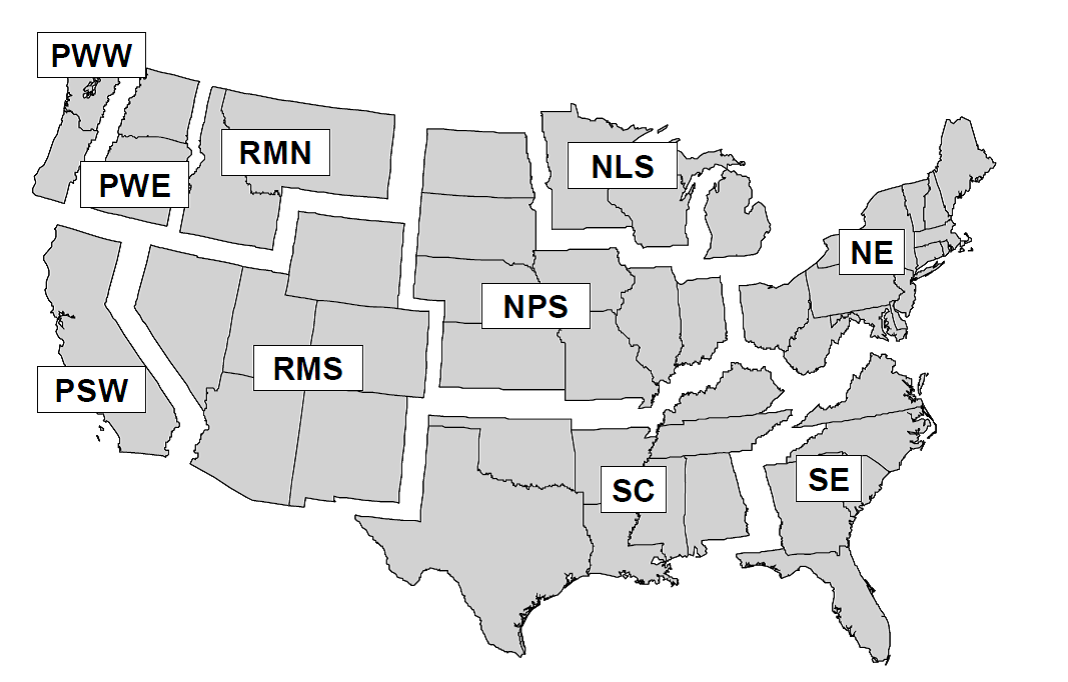
\includegraphics[width=1\linewidth]{images/regions_map} \caption{Definition of regions: Pacific Northwest, West (PWW); Pacific Northwest, East (PWE); Pacific Southwest (PSW); Rocky Mountain, North (RMN); Rocky Mountain, South (RMS); Northern Prairie States (NPS); Northern Lake States (NLS); Northeast (NE); South Central (SC); and Southeast (SE).  Note that regions are merged for some template files, these combinations include: NLS and NPS as North Central, RMN and RMS as Rocky Mountain; and RMN, RMSE, PWE and PSW as West. Source: Smith et al. (2006)}\label{fig:template-map-fig}
\end{figure}

Each template lacks harvest data and timber product ratios. The user
must provide these. We recommend searching for references similar to the
citations listed in the section above to revise or verify given values.
The \texttt{Natl\_datasets} folder contains a (U.S.) national template
that additionally lacks primary product ratios and the board foot to
cubic foot conversion factors. The other original templates based on
Smith et al. (\protect\hyperlink{ref-smith2006}{2006}) geographic
regions each have a unique primary products ratios data sheet (except
for the Pacific Southwest which shares values with the California input
file) that rely on Smith et al.
(\protect\hyperlink{ref-smith2006}{2006}) which in turn depends on
information from Adams (\protect\hyperlink{ref-adams2006}{2006}), and
therefore are likely based on mill surveys updated through 2005 at the
latest. We urge users to consider carefully whether they want to use
these included values. These ratios, as can be seen, are constant across
years. This is not the case for the California, Oregon, or Washington
data sets which contain a more detailed set of primary product ratios
that vary through time based on literature documenting historic and
current wood utilization. If the user has the resources to construct
more detailed primary product ratios for the area of analysis, that is
ideal.

Generic board foot to cubic foot volume conversions are provided in the
original regional templates that are the same for each region. These
values are only updated to 2007 and it is unclear what the data source
is for these values, though they appear to match the values developed
for the California inventory. We urge users to consider carefully
whether they want to use these included values. It is recommended
instead that, in the absence of user-provided data for these values,
users choose the board foot to cubic foot volume conversion provided in
the appropriate U.S. Forest Service Regional HWP C report (D. Loeffler
and K. Stockmann, personal communication, September 16, 2022). Some
regions used in this model overlap more than one U.S. Forest Service
region, as noted above. The original values and the recommended values
for each state within the model region are provided as notes within each
template. Users must decide which value to use and populate the
necessary fields in the template themselves.

We urge users to inspect the details and datasources provided in Section
@ref(own-prov-input) for each input parameter in the templates and
decide whether they want to use the included values, provide their own
values, or search for updated datasets.

When using a template to construct a data set, users may need to adjust
yearly ranges or values in any of the worksheets that come before or
after the target year values. \textbf{In other words, all datasets in
each worksheet of the template file must have the same number of years.}
For instance, the California harvest data begins in 1952. If I used the
Pacific Southwest template I would need to remove pre-1952 columns from
the worksheets TimberProdRatios, PrimaryProdRatios, EndUseRatios, and
DiscardFates, and adjust values on other worksheets. Section
@ref(own-prov-input) can be used as a checklist to ensure the right
changes are made to input data templates.

\hypertarget{own-prov-input}{%
\subsection{Creation of the input file}\label{own-prov-input}}

This explanation may work best if the user opens example files, such as
CA\_Inputs\_HWP\_Model.xlsx or Oregon\_Inputs\_HWP\_Model.xlsx, and
examines the files while reading the description of each worksheet.

\hypertarget{own-prov-input-options}{%
\subsubsection{Model options}\label{own-prov-input-options}}

Worksheet name: HWP\_TOOL\_OPTIONS

The first worksheet in the input data template file,
HWP\_MODEL\_OPTIONS, allows the user to customize the operation and
output of the HWP model. The values in this worksheet affect the
operation of the stand-alone model and/or the Shiny application.
Asterisks indicate options that all users should adjust if using the
Shiny web application and/or the stand-alone version of the model, with
the remainder as optional to adjust for advanced users:

\begin{itemize}
\item
  *DATASET.NAME (string): This value only affects the Shiny web
  application. This name will appear as an option in the upper-left
  pulldown menu in the application. Avoid using the names ``California''
  or ``Oregon'' as the application is pre-loaded with these datasets and
  it will be difficult to distinguish these from the user's dataset.
\item
  *QA\_TEST (TRUE, FALSE) -- This value only affects the stand-alone
  model. The default is TRUE. If TRUE, the stand-alone code will
  complete the QA check of the input data file and examine all
  worksheets except HWP\_MODEL\_OPTIONS to ensure the input file is set
  up with the correct number of years and types of values in all
  worksheets. See Section @ref(own-qa) below. If FALSE, the code will
  skip the QA step and attempt to load the worksheets without examining
  them. Little system time is needed to conduct the QA test.
\item
  OUTPUT\_ARRAYS (TRUE, FALSE) -- This value only affects the
  stand-alone model. If users would like the program to produce the
  analysis arrays so that they can trouble-shoot model issues or verify
  calculations, this value should be set to TRUE (default). Otherwise,
  FALSE. There is a noticeable time savings in code execution when this
  value is set to FALSE.
\item
  OUTPUT\_TABLES (TRUE, FALSE) -- This value only affects the
  stand-alone model. This option allows users to select whether the code
  produces output tables for the base HWP analysis. Default = TRUE.
\item
  SHIFTYEAR (TRUE, FALSE) -- Affects both the Shiny web application and
  stand-alone model. If the user wants tabular and figure outputs of
  emissions and pools reported as occurring the year after harvest as in
  the original USFS variants of the tool, this value should be TRUE. If
  the user wants those outputs reported as occurring during the same
  year as harvest, select FALSE. Note that outputs for intermediate
  arrays are not year-shifted.
\item
  PIU.WOOD.LOSS (Double, 0.00 to 1.00) -- Affects both the Shiny web
  application and stand-alone model. The current estimated loss factor
  specifying the quantity of carbon that is immediately discarded when
  solid wood products are placed into end-uses and enter the PIU pool is
  0.08, or 8\%. The default value is set to 0.08; enter a different
  value if you wish to alter the amount. The value cannot exceed 1.0 or
  fall below 0. For reference, Skog and Nicholson
  (\protect\hyperlink{ref-skog2000}{2000}) also cite a value of 5\% for
  paper.
\item
  PIU.PAPER.LOSS (Double, 0.00 to 1.00) -- Affects both the Shiny web
  application and stand-alone model. Our default loss factor specifying
  the quantity of carbon that is immediately discarded when pulp wood
  products (paper) are placed into end-uses and enter the PIU pool is
  set to 0.0; enter a different value if you wish to alter the amount.
  The value cannot exceed 1.0 or fall below 0.
\item
  ARRAYLOC (Text) -- This value only affects the stand-alone model. The
  default value is ``HWP\_Stand\_Alone\_Files/Arrays/''. If you wish to
  save arrays to a different folder, change the folder location value.
  If you are using Windows, be sure to use the forward slash ``/''
  between folder levels and not the back slash.
\item
  TABLELOC (Text) -- This value only affects the stand-alone model. The
  default value is ``HWP\_Stand\_Alone\_Files/Tables/''. If you wish to
  save tables to a different folder, change the folder location value.
  If you are using Windows, be sure to use the forward slash ``/''
  between folder levels and not the back slash.
\item
  *RUN.MC (TRUE, FALSE) -- This value only affects the stand-alone
  model. If you would like to run the Monte Carlo simulation on your
  data set, ensure that this value is TRUE. The main model code will run
  and then verify that this value is TRUE, at which time it will source
  the Monte Carlo R code and run it. Note: running the Monte Carlo
  simulation is very time consuming. Set this option to FALSE if you are
  running the stand-alone model and are not currently interested in the
  Monte Carlo output.
\item
  R (Numeric, between 0 to 1) -- Affects both the Shiny web application
  and stand-alone model. This value is the target Pearson's correlation
  coefficient that will be used to correlate triangular distribution
  values in the Monte Carlo. For instance, if the worksheet
  MonteCarloDistrParameters has three accuracy values for Harvest,
  depending on the year of harvest, the value for R will determine how
  correlated the three random draws are that are used to adjust the
  Harvest values for each iteration. The default is 0.5, as was used in
  Stockmann et al. (\protect\hyperlink{ref-stockmann2012}{2012}).
\item
  OPT.START.VALUE (Numeric, between 0 and 1) -- Affects both the Shiny
  web application and stand-alone model. The MonteCarloDistrParameters
  states minimum and maximum 90\% Confidence Intervals from which the
  Monte Carlo random variables are to be drawn. However, when we
  transform random uniform values into values from a triangular
  distribution, we need to know the triangular distribution endpoints.
  In the Monte Carlo code, the function ``ab.boundaries.fcn'' performs a
  search algorithm to find the triangular distribution end points given
  the confidence intervals provided in the MonteCarloDistrParameters
  worksheet. The default start value for the algorithm is 0.5 and likely
  does not need to be altered for the Monte Carlo code to function
  adequately.
\item
  *N.ITER (Integer, 1 or greater) -- Affects both the Shiny web
  application and stand-alone model. This value determines the number of
  iterations the Monte Carlo performs. In the Shiny application, the
  Monte Carlo Estimates selection ``Monte Carlo convergence estimation''
  produces convergence plots that track estimates for the last year
  examined in the model. The plot shows the values for the mean,
  standard error, and 95\% and 5\% Confidence Intervals given the
  iterations performed. Of the four, the Mean is most informative. If
  the line is stable for many iterations (we seem to obtain fairly
  stable results with 2000 iterations) then you likely have a sufficient
  number of iterations. The more iterations, the slower the code will
  run. Too few iterations will provide unreliable results. The default
  value is currently 100 runs which is likely too few but is sufficient
  to verify that the process works. 1000 to 2000 might be a recommended
  number for obtaining reliable estimates.
\item
  MC.ARRAY.OUT (TRUE, FALSE) -- This value only affects the stand-alone
  model. If TRUE, the Monte Carlo code will generate the (large)
  Microsoft Excel workbook MC\_All.xlsx that contains all MMTC values
  for each year and each iteration of the Monte Carlo code. There is a
  separate tab for Emitted with Energy Capture (eec), Emitted Without
  Energy Capture (ewoec), Solid Waste Disposal Sites carbon (swdsC), and
  Products in Use (pu). The default is TRUE; if it is FALSE the code
  will run a bit faster and the large (\textasciitilde10 MB?) file will
  not be produced. The file is provided for model assessment purposes.
\end{itemize}

\hypertarget{own-prov-input-harvest}{%
\subsubsection{Harvest}\label{own-prov-input-harvest}}

Worksheet name: HARV\_MBF

The worksheet Harvest\_MBF contains a time series of total yearly
harvest values in thousand board feet (MBF). Annual harvest time series
are provided for California, Oregon and Washington. Otherwise,
\emph{this worksheet must be populated by the user}. The user may choose
to analyze an entire historic annual harvest time series dataset or only
a subset of years. Analyzing a different number of years will provide a
different picture of trends in storage and emissions than modeling the
entire period. This is due both to the annual harvest quantities and
utilization and disposal parameters, which vary over time.

The yearly harvest is the total annual harvest from the region or owner
of interest, entered in MBF. The left column must contain the heading
``Year'' and have years listed in sequential order from least to
greatest. Ownership columns may follow, with a final column entitled
``Total'' that must equal the ownership values. Users may omit all but
the Year and Total columns. Users may have ownership values appear at
some point after the first year of total harvest values; however, leave
the ownership cells prior to the first year of ownership values blank
and not filled with zeros. The QA check sums the values to determine if
they equal the total value, so a series of zeros obviously will cause
the QA check to fail.

Data sources used for California timber harvest include Bolsinger
(\protect\hyperlink{ref-bolsinger1976}{1976}),
\href{https://www.blm.gov/programs/natural-resources/forests-and-woodlands/timber-sales/bureau-wide-timber-data}{BLM
Bureau Wide Timber Data}, Morgan
(\protect\hyperlink{ref-morgan2004}{2004}), Morgan et al.
(\protect\hyperlink{ref-morgan2012}{2012}), McIver et al.
(\protect\hyperlink{ref-mciver2015}{2015}),
\href{https://www.fs.fed.us/forestmanagement/products/cut-sold/index.shtml}{USFS
Cut-and-Sold-Reports}, and Warren
(\protect\hyperlink{ref-warren2005}{2005}). Specific data sources for
Oregon and Washington annual harvest time series are provided in Morgan
et al. (\protect\hyperlink{ref-morgan2021}{2021}) and Nichols et al.
(\protect\hyperlink{ref-nichols2020}{2020}).

\hypertarget{own-prov-input-bfcf}{%
\subsubsection{BF to CF conversion factors}\label{own-prov-input-bfcf}}

Worksheet name: BFCF

The worksheet BFCF contains the conversion factors between board feet
and cubic feet for various time periods. Additional calculations are
completed in the R code to account for harvest volumes being provided in
thousand board feet (MBF) and subsequent model calculations occurring on
units of hundred cubic feet (CCF). Factors used to convert BF to CF vary
by time and place. Conversions are based on Scribner log scale rather
than lumber scale rules.

Generic conversions are provided in the original regional templates that
are the same for each region. These values are only updated to 2007 and
it is unclear what the data source is for these values. We urge users to
consider carefully whether they want to use these included values. It is
recommended instead, that in the absence of user-provided data for these
values, users choose the BF to CF volume conversion provided in the
appropriate U.S. Forest Service Regional HWP C report (D. Loeffler and
K. Stockmann, personal communication, September 16, 2022). Note that
there is only a single value provided for the entire time series. Some
regions used in this model overlap more than one U.S. Forest Service
region, as noted above. The original values and the recommended values
for each state within the model region are provided as notes within each
template. Users must decide which value to use and populate the
necessary fields in the template themselves. Ideally the user provides
local or regional values and updates the values whenever relevant mill
surveys are completed.

The user may choose to change these conversion factors when mill surveys
are updated or if more detailed information is available by region
spanning any given time series. There are only three columns,
Conversion, StartYear, and EndYear to specify the conversion value and
the starting and ending year of harvest data the conversion applies to.
Ensure that the first Start Year begins with the minimum Harvest\_MBF
Year and that conversion time periods do not overlap. When mill surveys
are completed, ratios are applied from the year of the latest survey
backwards to the last survey (note that in the WA template, ratios are
applied from the year of the latest survey \emph{forwards} to the next
survey). For example, the BF to CF ratio from the California mill survey
for 2012 is applied from 2012 backwards to 2007, as the previous mill
survey was completed in 2006. The most recent California mill survey for
2016 results in a BF to CF ratio applied from 2016 backwards to 2013.
This ratio is also applied forwards to the present until a new mill
survey is completed and this ratio can be updated for 2017 forward. The
final end year must be the same as the final year annual harvest data is
provided for in the worksheet named ``Harvest\_MBF.'' The Conversion
column values are formatted as doubles and StartYear and EndYear values
are integers.

Data sources for CA/USFS Pacific Southwest region ratios were obtained
from Keegan et al. (\protect\hyperlink{ref-keegan2010}{2010}) (1952 --
1989), Morgan (\protect\hyperlink{ref-morgan2004}{2004}) (1990 -- 2000),
Morgan et al. (\protect\hyperlink{ref-morgan2012}{2012}) (2001 -- 2006),
McIver et al. (\protect\hyperlink{ref-mciver2015}{2015}) (2007 -- 2016),
and Marcille et al. (\protect\hyperlink{ref-marcille2020}{2020})
(2013-present). Specific data sources for Oregon and Washington annual
harvest time series are provided in Morgan et al.
(\protect\hyperlink{ref-morgan2021}{2021}) and Nichols et al.
(\protect\hyperlink{ref-nichols2020}{2020}).

Default BF to CF conversion factors provided for the rest of the U.S.
from the original USFS HWP C version of the tool only exist up to 2007
and are extrapolated beyond 2007. Additionally, this data set's data
sources are unclear. The recommended regional defaults provided in each
template were obtained from the following U.S. Forest Service Regional
HWP C reports: Butler, Stockmann, Anderson, Skog, et al.
(\protect\hyperlink{ref-butler2014nw}{2014}), Butler, Stockmann,
Anderson, Young, et al. (\protect\hyperlink{ref-butler2014sw}{2014}),
Loeffler et al. (\protect\hyperlink{ref-loeffler2014er}{2014a}),
Loeffler et al. (\protect\hyperlink{ref-loeffler2014sr}{2014b}),
Stockmann et al. (\protect\hyperlink{ref-stockmann2014nr}{2014a}),
Stockmann et al. (\protect\hyperlink{ref-stockmann2014imr}{2014c}),
Stockmann et al. (\protect\hyperlink{ref-stockmann2014rmr}{2014b})

\hypertarget{own-prov-input-tpr}{%
\subsubsection{Timber Product Ratios}\label{own-prov-input-tpr}}

Worksheet name: TimberProdRatios

The worksheet TimberProdRatios contain the timber product ratios, or
TPR. The yearly timber product ratios represent the portion of the
annual harvest that is classified as specific timber products, such as
sawtimber, pulpwood, posts, and fuelwood. Default TPRs are provided for
California, Oregon and Washington. \textbf{Otherwise, this worksheet
must be populated by the user}.

The first column must be TimberProductID, which is a numerical
identifier of the timber product category name. Timber product category
names are specified in the worksheet named ``RatioCategories'' (Section
@ref(own-prov-input-rc)). The remainder of the columns are named after
the sequential years of harvest data, from the earliest year to the
final year. The number of years in this dataset must match the number of
years annual harvest data is provided for in the worksheet named
``Harvest\_MBF''. All year-column values must sum to one. Row values may
change over time. When mill surveys are completed, ratios are applied
from the year of the latest survey backwards to the last survey (note
that in the WA template, ratios are applied from the year of the latest
survey \emph{forwards} to the next survey). Most recent available
records may also need to be extended forwards if data for recent years
of analysis do not yet exist. For example, the TPRs from the California
mill survey for 2012 is applied from 2012 backwards to 2007, as the
previous mill survey was completed in 2006. The most recent California
mill survey for 2016 results in a set of TPRs applied from 2016
backwards to 2013. This ratio is also applied forwards to the present
until a new mill survey is completed and this ratio can be updated for
2017 forward.

Data sources for California TPR and PPR include Barrette, Gedney, and
Oswald (\protect\hyperlink{ref-barrette1970}{1970}), Hiserote and Howard
(\protect\hyperlink{ref-hiserote1978}{1978}), Howard
(\protect\hyperlink{ref-howard1974}{1974}), Marcille et al.
(\protect\hyperlink{ref-marcille2020}{2020}), McIver et al.
(\protect\hyperlink{ref-mciver2015}{2015}), Morgan
(\protect\hyperlink{ref-morgan2004}{2004}), Morgan et al.
(\protect\hyperlink{ref-morgan2012}{2012}), Ward
(\protect\hyperlink{ref-ward1995}{1995}), and Ward
(\protect\hyperlink{ref-ward1997}{1997}). The original model templates
for the nine US regions (see Figure @ref(fig:template-map-fig)) rely on
Smith et al. (\protect\hyperlink{ref-smith2006}{2006}) which in turn
depends on information from Adams
(\protect\hyperlink{ref-adams2006}{2006}), and therefore are likely
based on mill surveys updated through 2005 at the latest.

\hypertarget{own-prov-input-ppr}{%
\subsubsection{Primary Product Ratios}\label{own-prov-input-ppr}}

Worksheet name: PrimaryProdRatios

The worksheet PrimaryProdRatios contain the primary product ratios, or
PPR. The yearly primary products ratios represent the portion of each
yearly timber product that is used in specific primary products, such as
lumber, wood pulp, plywood, and fuelwood. Default PPRs are provided for
California, Oregon and Washington, as well as the defaults from the
original USFS version of the tool for the nine US regions (see Figure
@ref(fig:template-map-fig)). Default PPRs for the nine US regions are
constant across the years, whereas the California, Oregon and Washington
PPRs contain a more detailed set of primary product ratios that vary
through time based on literature documenting historic and current wood
utilization. \textbf{Otherwise, this worksheet must be populated by the
user}. If the user has the resources to construct more detailed primary
product ratios for the area of analysis, that is ideal. The first column
in the worksheet must be PrimaryProductID, which is a numerical
identifier of the primary product category name. Primary product
category names are specified in the worksheet named ``RatioCategories''
(Section @ref(own-prov-input-rc)). The remainder of the columns are
named after the sequential years of harvest data, from the earliest year
to the final year. The number of years in this dataset must match the
number of years annual harvest data is provided for in the worksheet
named ``Harvest\_MBF''. All year-column values must sum to the number of
TPR rows (e.g., 40 TPR categories for California and Oregon data). Sets
of PPR ratios sum to 1; most sets include only one ratio. For instance,
California and Oregon data set PPR IDs 1-7, 8-14, 15-21, and 22-28 sum
to 1. Row values may change over time.

Note that sets of PPRs did not sum to 1 in some of the original regional
templates. In some cases, these values were off by hundredths or
thousandths and were manually updated. These rows are highlighted in
yellow and comments are provided in the cells of the templates where
these manual adjustments were made. In other cases some PPR set values
were set to 0, likely because in those regions (i.e., PNW-E, Rocky
Mountain, West) the timber product associated with those primary
products did not exist (e.g., timber product hardwood sawtimber or
hardwood pulpwood). However, in this case the TPRs should be set to 0
rather than the PPRs. For the model code to run correctly, the PPR sets
must sum to 1. Where the discrepancy existed, these values were manually
updated. These worksheets are highlighted in red and comments are
provided in the cells of the templates where these manual adjustments
were made.

Data sources for California TPR and PPR include Barrette, Gedney, and
Oswald (\protect\hyperlink{ref-barrette1970}{1970}), Hiserote and Howard
(\protect\hyperlink{ref-hiserote1978}{1978}), Howard
(\protect\hyperlink{ref-howard1974}{1974}), Marcille et al.
(\protect\hyperlink{ref-marcille2020}{2020}), McIver et al.
(\protect\hyperlink{ref-mciver2015}{2015}), Morgan
(\protect\hyperlink{ref-morgan2004}{2004}), Morgan et al.
(\protect\hyperlink{ref-morgan2012}{2012}), Ward
(\protect\hyperlink{ref-ward1995}{1995}), and Ward
(\protect\hyperlink{ref-ward1997}{1997}). The original model templates
for NFS Region 9 rely on Smith et al.
(\protect\hyperlink{ref-smith2006}{2006}) which in turn depends on
information from Adams (\protect\hyperlink{ref-adams2006}{2006}), and
therefore are likely based on mill surveys updated through 2005 at the
latest.

\hypertarget{own-prov-input-eur}{%
\subsubsection{End Use Ratios}\label{own-prov-input-eur}}

Worksheet name: EndUseRatios

The worksheet EndUseRatios contains end use ratios, or EUR. End-use
product ratios determine the annual distribution of primary wood
products, such as lumber and non-structural panels, to end-uses, such as
single family new housing and furniture manufacturing. These ratios
determine the end-use each primary product is associated with. The
end-use is important to know because it will determine the time the
carbon remains in the PIU pool prior to discard based on end-use product
half-lives discussed in Section @ref(own-prov-input-euhl). National
default EURs are provided. It is unnecessary for the user to modify
these ratios unless the national dataset is updated or users want to
explore hypothetical wood utilization scenarios.

The distribution of each primary product among end-uses must sum to 1.0.
The program will only work if each primary products end-use distribution
sums to 1.0. The first column must be EndUseID, which is a numerical
identifier for the end-use category name. End-use category names are
specified in the worksheet named ``RatioCategories'' (Section
@ref(own-prov-input-rc)). The remainder of the columns are named after
the sequential years of harvest data, from the earliest year to the
final year. The number of years in this dataset must match the number of
years annual harvest data is provided for in the worksheet named
``Harvest\_MBF''. All year-column values must sum to the number of PPR
rows. Row values may change over time. \emph{Currently values for the
last year for which data are available (2009) are applied forward for
all subsequent years to the present. However, 2009 was in the tail end
of the Great Recession and may not be representative of more recent
years. Users may want to use EURs from a year just prior to the
recession, such as 2006, for more recent analysis years. On the other
hand, using 2006 EUR values would not reflect the changes in milling
opportunities that may have occurred after the recession.}.

National end-use ratios were obtained from McKeever
(\protect\hyperlink{ref-mckeever2009}{2009}) and McKeever and Howard
(\protect\hyperlink{ref-mckeever2011}{2011}) and were last updated
through 2009.

\hypertarget{own-prov-input-rc}{%
\subsubsection{Ratio Categories}\label{own-prov-input-rc}}

Worksheet name: RatioCategories

The worksheet RatioCategories acts as a link between TPR, PPR, and EUR
categories specified numerically in the TPR, PPR and EUR worksheets. The
first three column labels, TimberProductID, PrimaryProductID, and
EndUseID, must have the same names as the respective first columns of
the previous three worksheets described. The fourth through sixth column
names are TimberProduct, PrimaryProduct, and EndUseProduct, and contain
text describing what the categories contain. Note that EndUseProduct is
a subcategory of PrimaryProduct, and PrimaryProduct is a subcategory of
TimberProduct. The R code ignores columns 4 through 6; they are there
for assisting users in identifying row values. The user does not need to
change these values unless they change the number of TPR, PPR, and/or
EUR categories. It is unnecessary for the user to update these
categories unless the number of timber product, primary product, or
end-use categories change either due to updated data or for hypothetical
wood utilization scenario exploration.

\hypertarget{own-prov-input-ccfMTC}{%
\subsubsection{CCF to metric tons carbon}\label{own-prov-input-ccfMTC}}

Worksheet name: CCF\_MT\_Conversion

The worksheet CCF\_MT\_Conversion contains factors to convert CCF
volumes of individual primary products to metric tons of carbon.
National default values are provided. These factors were last updated in
2005. It is unnecessary for the user to update these values unless the
national conversion factors are updated or local/regional factors are
developed based on the harvest species mix in the area of analysis.

The first column title must be PrimaryProductID, and the second column
CCFtoMTconv. The first column values must be integers and include all
primary product ratio categories.

The conversion factors were obtained from Smith et al.
(\protect\hyperlink{ref-smith2006}{2006}) and Skog
(\protect\hyperlink{ref-skog2008}{2008}).

\hypertarget{own-prov-input-euhl}{%
\subsubsection{End-use product half-lives}\label{own-prov-input-euhl}}

Worksheet: EU\_HalfLives

End-use product half-life values express the decay rate at which carbon
in the products in use category passes into the Discarded Products
category. National default values are provided. It is unnecessary for
the user to update these values unless the national conversion factors
are updated or the user wants to explore hypothetical changes to the
functional lifespan of products. The user may choose to change any
half-life of the 224 primary product end-uses. The user may alter as few
or as many half-lives as desired. Increasing end-use half-lives will
result in carbon storage in the Products in Use pool for a longer time
period, while decreasing half-lives will pass those end-use products
into the Discarded Products category at a faster rate. It is unclear if
or how often the end-use half life values should be updated.

The worksheet EU\_HalfLives contains half-life values (in years) for
each of the end use categories. The first column must be titled
EndUseID, the second EU\_HalfLife. The values for EndUseID must be
integers and include all end use ratio categories.

References for end-use product half-lives are listed in and were
obtained from Smith et al. (\protect\hyperlink{ref-smith2006}{2006}). In
turn, Smith et al. (\protect\hyperlink{ref-smith2006}{2006}) cites Skog
and Nicholson (\protect\hyperlink{ref-skog1998}{1998}), Skog and
Nicholson (\protect\hyperlink{ref-skog2000}{2000}) (which is identical
to Skog and Nicholson (\protect\hyperlink{ref-skog1998}{1998})), and Row
and Phelps (\protect\hyperlink{ref-row1996}{1996}). Not all end-use
half-lives used in the tool appear to have published half-lives. Some
half-lives used for one product category were assumed to be sufficient
for others that lacked data. A forthcoming general technical report from
the USFS documents these apparent assumptions
(\protect\hyperlink{ref-lucey202X}{Lucey et al. In review}).

\hypertarget{own-prov-input-discFates}{%
\subsubsection{Discard products disposition
ratios}\label{own-prov-input-discFates}}

Worksheet name: DiscardFates

In any given inventory year wood and paper from every single vintage
year passes from the Products in Use pool into the Discarded Products
category. The worksheet DiscardFates contains values that apportions
discarded carbon to different discard categories: DEC = Discard Energy
Capture, BWoEC = Burned Without Energy Capture, Recovered, Composted,
Landfills, and Dumps. Paper (defined by the code as primary products
where the column EndUseProduct in the worksheet RatioCategories contains
the word ``pulp'') and solid wood products are allowed to have different
discard ratio values. The first two columns must be named DiscardType
and DiscardDestination. The remainder of the column titles are the
years, in order, from longest ago to most recent. The number of years in
this dataset must match the number of years annual harvest data is
provided for in the worksheet named ``Harvest\_MBF''. The sum of each
year-column should be two (all wood and all paper values within a column
should sum to one). Row values may change over time.

All default wood and paper products discarded disposition ratios were
obtained from Skog (\protect\hyperlink{ref-skog2008}{2008}). These data
represent a (U.S.) nationwide dataset that has not been updated since
2005. These data could be updated, from either national databases or
local/regional datasets from relevant waste characterization studies.
Skog (\protect\hyperlink{ref-skog2008}{2008}) cites HWP dump and
landfill data from Freed (\protect\hyperlink{ref-freed2004}{2004}) which
is an unpublished spreadsheet that made use of data from US EPA
(\protect\hyperlink{ref-epa2006}{2006}), Melosi
(\protect\hyperlink{ref-melosi1982}{1982}), and Melosi
(\protect\hyperlink{ref-melosi1999}{1999}). It is unnecessary for the
user to update unless the national dataset is updated, data is developed
at the regional or local level for relevant waste characterization
studies, or the user wants to explore hypothetical scenarios. The
national data set is in the process of being updated with more recent
data (i.e., US EPA (\protect\hyperlink{ref-usepa2020}{2020})) to cover
the period from 2005-2020. The user may alter as few or as many discard
ratios as desired. Altering ratios can affect the quantity of HWPs that
are emitted with and without energy capture at the end of their
functional lifespan.

It should be noted that some of the HWP discarded into the SWDS may be
burned for disposal in a boiler with energy capture (DEC; e.g., a trash
incinerator). The proportion (values between 0 and 1) of discarded HWP
with energy capture (DEC) guides what portion of discarded HWP is burned
for energy capture for every year of the time series. There are no
default proportions in the model; or rather, the default is 0. Values
used for the DEC rows must be between 0 and 1 (e.g., 0.5 = 50\%
discarded wood is burned with energy capture). Adjusting proportions
affect only HWP that have been discarded and is not related to the
fuelwood component of HWP. Currently, we only provide a test data set
(CA\_DiscardEnergyCapture\_Test.xlsx, see Section @ref(dnld-files)) that
includes DEC proportions. Users could update the values with national or
regional waste characterization or other waste disposal data.

\hypertarget{own-prov-input-discHL}{%
\subsubsection{Discarded products disposition half-lives and landfill
fixed ratios}\label{own-prov-input-discHL}}

Worksheet name: Discard\_HalfLives

Discarded products disposition half-lives are the half-lives of wood and
paper, which vary between landfills, dumps, and recovered (recycled)
products. These values determine the quantity and rate HWPs are emitted
with and without energy capture at the end of their functional lifespan.
The worksheet Discard\_HalfLives provides half-life values in years for
paper and wood in dumps (Dumps), recovered products (Recovered), and the
decaying portion of landfills (Landfills\_decay). A single value is
provided for each category. It also, possibly confusingly, includes
values for the proportion of wood and paper that end up in the
non-decaying portion of landfills (Landfills\_fixed). The columns must
be labeled Type, Dumps, Landfills\_fixed, Landfills\_decay, and
Recovered.

Discard ratios and landfill fixed carbon ratios are provided based on
national or international defaults. It is unnecessary for the user to
update the defaults unless international or national datasets are
updated, local/regional data is identified, or the user wants to explore
hypothetical scenarios.

The user may choose to change any half-life of wood and paper products
that are in landfills, dumps, or recovered (recycled) as well as the
landfill fixed ratios. The user may alter as few or as many half-lives
as desired. Increasing half-lives will result in slower carbon decay and
will increase the recalcitrance time of carbon in Solid Waste Disposal
Sites (SWDS). Decreasing half-lives will result in faster carbon decay
and will decrease the recalcitrance time of carbon in SWDS. Increasing
the landfill fixed carbon ratios will increase the amount of carbon that
is not subject to decay and therefore decrease landfill emissions.
Decreasing these ratios would have the opposite effect. \emph{Please
note, current defaults for landfill fixed carbon ratios have not been
updated in the templates to the current, higher IPCC 2019 refinement
defaults (\protect\hyperlink{ref-buendia2019}{Buendia et al. 2019}). The
next state-level inventories for Oregon and California will reflect
these updated values.}

Data sources for Landfill, dumps, and recovered (recycled) wood and
paper half-lives are listed in Skog
(\protect\hyperlink{ref-skog2008}{2008}). Information for dumps in Skog
(\protect\hyperlink{ref-skog2008}{2008}) cites Table 5.7 in Penman et
al. (\protect\hyperlink{ref-penman2000}{2000}). For landfills, Skog
(\protect\hyperlink{ref-skog2008}{2008}) cites Table 3.4 in Buendia et
al. (\protect\hyperlink{ref-buendia2019}{2019}). For recovered products
Skog (\protect\hyperlink{ref-skog2008}{2008}) cites Pingoud et al.
(\protect\hyperlink{ref-pingoud2006}{2006}).

However, the value in Pingoud et al.
(\protect\hyperlink{ref-pingoud2006}{2006}) is not what was included in
the original USFS versions of the tool and the value that was included
appears to match the paper half-life presented in Smith et al.
(\protect\hyperlink{ref-smith2006}{2006}).

For the landfill fixed carbon ratio information, Skog
(\protect\hyperlink{ref-skog2008}{2008}) which cites Freed and Mintz
(\protect\hyperlink{ref-freed2003}{2003}) who in turn use data from
Barlaz (\protect\hyperlink{ref-barlaz1998}{1998}) and Eleazer et al.
(\protect\hyperlink{ref-eleazer1997}{1997}). Users may choose to update
the ratios using information provided in the 2019 IPCC refinement
(\protect\hyperlink{ref-ruter2019}{Rüter et al. 2019}).

\hypertarget{own-prov-input-mc}{%
\subsubsection{Monte Carlo values}\label{own-prov-input-mc}}

Worksheet name: MonteCarloValues

The worksheet MonteCarloValues allows users to define how much variation
to introduce into the HWP model for the Monte Carlo simulation. The
outcomes of the simulation are summarized as statistical confidence
intervals for carbon storage (PIU, SWDS pools, and both pools combined)
and carbon emissions (with and without energy capture). This worksheet
also allows the user to specify aspects of the Monte Carlo that they
would like to control. The worksheet needs to be altered to conform to
the user's data structure for the Monte Carlo to run. That is, if users
have data from 1970 -- 2018, they will need to change First\_Year and
Last\_Year values for some of the rows. Default distributions were
obtained from Stockmann et al.
(\protect\hyperlink{ref-stockmann2012}{2012}). It is unnecessary to
change the defaults unless the user has more details on the range of
uncertainty for the various parameters used in HWP carbon estimation.
Users can change First\_Year, Last\_Year, MinCI, MaxCI, and CI values.
They may add or delete rows for Harvest, TimberProdRatios, and
PrimaryProdRatios. Each row of the worksheet represents a vector of
random draws, with one random draw per iteration. If our model had 100
iterations and this worksheet had 20 rows, the R script will obtain 2000
random uniform draws between zero and one, 100 random values per row.
(Please use more than 100 iterations for your final runs.) The R script
will change these values to triangular distributions with a peak at 1.0
(column Peak Value) and lower and upper confidence intervals as defined
by the columns MinCI and MaxCI. The resulting random numbers for a given
parameter (row) will have values that are above or below 1.0. In
general, the parameter values associated with each of the parameters are
multiplied by the random number for a single iteration. If the random
number is 0.86, the parameter value will be reduced to 86\% of its
original size. Below we describe each of the columns and column values
in this worksheet.

\begin{itemize}
\item
  Parameter\_ID: This column is included for the user's information; the
  R script does not rely upon it. Each of the parameters to be altered
  is listed here. Some parameters (namely, those after Parameter ID
  number 13) may have more than one set of random numbers generated for
  it. For instance, if we wish for Harvest values to be modeled as
  becoming more accurate through time, reflecting improvements in
  reporting and data collection, we may wish to indicate three periods
  of years with increasing estimate precision. A series of random
  numbers will be drawn for each of the time periods, and then
  correlated (see above). Within an iteration, this example would have
  three correlated random numbers that would be used for the three
  periods of years. The parameter ID for Harvest would be the same
  number repeated three times (14, 14, 14).\\
\item
  Parameter\_Name: The column name, ``Parameter Name'', is not used by
  the code. However, the column values are names for specific parameters
  that are used by the code. These must remain unchanged. The names can
  be repeated as necessary (following on the example for Parameter ID,
  Parameter ID 14, 14, 14 would be associated with Parameter Name
  ``Harvest'', ``Harvest'', ``Harvest''). Below are descriptions of
  which parameters and worksheets each relates to:

  \begin{itemize}
  \item
    CCFtoMTC: This name translates as ``hundred cubic feet converted to
    metric tons carbon''. Each Monte Carlo iteration will alter the
    conversion values associated with the worksheet CCF\_MT\_Conversion
    to reflect the level of uncertainty in the primary product volume to
    carbon conversion factors.
  \item
    EndUse\_HalfLives: Each Monte Carlo iteration's random number for
    this parameter will adjust the end use half life values found in
    EU\_halflives to reflect the level of uncertainty in the end-use
    half-lives.
  \item
    EndUseRatios: This variable refers to the end use ratio values found
    in the worksheet EndUseRatios. Each iteration of the Monte Carlo
    will use one random value to change the end use ratio values. See
    the discussion of the ``Sum-To-One Constraint'' in Section
    @ref(model-mc-samphwp) to understand how the values are altered.
    This is designed to reflect the uncertainty in the end-use ratios.
  \item
    DiscardedDispositionRatios, Paper: There are two rows in the
    Parameter Name column with the name DiscardedDispositionsRatios. The
    adjacent column, ``Paper'', indicates whether these disposition
    ratios are for paper (1) or wood (0). The disposition ratios are
    from the worksheet DiscardFates. They determine what fraction of
    paper or wood enter the categories of Discard Energy Capture, Burned
    Without Energy Capture, Recovered, Composted, Landfills, or Dumps.
    Like End Use Ratios, these ratios are subject to the sum-to-one
    constraint. Each Monte Carlo iteration alters the values of the
    discard ratios.
  \item
    LandfillDecayLimits: The wood and paper values represent the
    landfill decay limits, or the proportion of landfill material that
    is subject to decay. The values are obtained from the worksheet
    Discard\_HalfLives. The adjacent column, ``Paper'', indicates
    whether these disposition ratios are for paper (1) or wood (0). Each
    Monte Carlo iteration alters the values of the landfill fixed carbon
    ratios.
  \item
    Landfill\_HalfLives, Dump\_HalfLives, Recovered\_HalfLives: The six
    rows with these parameter names are associated with wood and paper
    decomposition half-lives for materials subject to decay in
    landfills, dumps, and in recovered products. The values are obtained
    from the worksheet Discard\_HalfLives. The adjacent column,
    ``Paper'', indicates whether these disposition ratios are for paper
    (1) or wood (0). Each Monte Carlo iteration alters the values of
    these decay ratios.
  \item
    Harvest: This parameter references the cubic-foot volume amounts
    harvested each year. The values are originally provided as board
    feet from the worksheet Harvest\_MBF, but they are transformed to
    unis of CCF in the original (non-Monte Carlo) portion of the
    analysis and the transformed values are used in the Monte Carlo.
    Each Monte Carlo iteration alters the values of the annual harvest
    volume estimates. There may be more than one row labeled as Harvest,
    reflecting different accuracies to be used for different
    year-ranges.
  \item
    TimberProdRatios: Like Harvest, there may be more than one entry for
    TimberProdRatios. The original worksheet is TimberProdRatios. Like
    EndUseRatios, a random value associated with a range of years will
    alter some, but not all, Timber Product Ratio values. See the
    discussion of the ``Sum-To-One Constraint'' in Section
    @ref(model-mc-samphwp). Each Monte Carlo iteration alters the values
    of the timber product ratios.
  \item
    PrimaryProdRatios. This type of parameter is altered much the same
    as TimberProdRatios and the original values may be found in the
    worksheet PrimaryProdRatios. It too is subject to the ``Sum-To-One
    Constraint''. Each Monte Carlo iteration alters the values of the
    primary product ratios.
  \end{itemize}
\item
  Paper: As described above for DiscardedDispositionRatios and other
  parameters, some parameters represent paper (1) or wood (0) for their
  associated parameters.
\item
  First Year, Last Year: These are values that users must change. The
  values in these columns represent the first year and last year of a
  given year period. For instance, if our data set included harvest from
  1906 to 2017 but we wanted to increase the precision of the Monte
  Carlo values in steps leading to the final year, then we need to
  indicate what years each level of precision refers to. If only one
  level of precision is used, provide the first year of harvest (e.g.,
  1906) under the First Year column and the last year of harvest (2017)
  to the Last Year column. If there are three Harvest rows, we want the
  First Year to capture all beginning years for given year periods and
  Last Year to capture the terminal year. For the first Harvest we might
  have First and Last Year values of 1906 and 1945, then in the second
  row the values 1946 and 1979, and finally the third row would contain
  a First Year of 1980 to 2017. Crucially: the very first First Year
  must be the first year of your harvest values, whether for Harvest,
  TimberProdRatios, or PrimaryProdRatios. There must not be overlap in
  years (e.g., if the first row had 1906 to 1945 and the next row had
  1941 to 1955, the sets would overlap). There must not be gaps (e.g.,
  1906 to 1945, then 1947 to 1955, leaving out 1946). You do not have to
  have the same sets of years used among parameter types (e.g., Harvest
  year sets do not need to match TimberProdRatios year sets). You do not
  need parameter types to have the same number of sets (Harvest could
  have two rows, PrimaryProdRatios could have three). You may have more
  or fewer than three year-sets per parameter type.
\item
  MinCI, Peak Value, MaxCI: As described above, these values are used to
  define the triangular distributions from which the random Monte Carlo
  values will be generated. For these three columns, Peak Values should
  all be 1.0, with the MinCI and MaxCI symmetric around this value (the
  Monte Carlo code assumes symmetric triangular distributions). That is,
  the MinCI and MaxCI must differ from the Peak Value by the same amount
  (e.g., MinCI = 0.85, Max CI = 1.15. Both are 0.15 distant from 1.0).
  The MinCI and MaxCI are the user-specified confidence intervals; e.g.,
  the user states what they wish the confidence intervals should be
  around 1.0.
\item
  CI: This value allows the user to change what sort of a confidence
  interval is used. The default value is a 90\% confidence interval, as
  was used in Stockmann et al.
  (\protect\hyperlink{ref-stockmann2012}{2012}). The user could change
  this value to 0.95, or a 95\% confidence interval. This sort of
  adjustment will affect the spread of the triangular distribution, with
  a 90\% confidence interval having a wider spread.
\end{itemize}

\hypertarget{own-qa}{%
\section{The quality assurance step}\label{own-qa}}

The Quality Assurance (QA) step is mandatory for data brought into the
Shiny web application and optional for the stand-alone program (see
above: QA\_TEST = TRUE/FALSE). The QA code, QA\_Code\_Shiny.r, assesses
the imported Excel file data. The QA step has over 55 checks it performs
on the incoming data to help ensure that the program will run correctly.
As it runs through its checks, it populates the file Error\_Report.csv
in the QA folder with results. It first verifies that it can load a
worksheet and then conducts subsequent tests on it. The code performs
tasks such as verifying that column labels are correct and that years
and TPR/PPR/EUR categories match among files. If it finds an error, it
will record a ``1'' in the Terminate column that matches the issue at
hand and describe the problem in the Comments column. If no problem is
found the Comments column will indicate which checks it made and found
correct. A zero in the Comments column may be ignored. If an error is
found, the R session will terminate (stand-alone model) or an error
message will be produced preventing further analysis (Shiny
application). This is on purpose! It prevents the code from attempting
to proceed. If termination occurs, check the error report to find out
which worksheet was triggering the error and why. Below we describe the
attributes that are checked for each worksheet:

\textbf{All 10 worksheets}: The QA code verifies that each worksheet
correctly loaded. A misspelling of the worksheet name will trigger a
terminal error.\\
Havest\_MBF:

\begin{itemize}
\tightlist
\item
  The first and last column names must be "Year" and "Total".\\
\item
  Values are numeric.\\
\item
  The sum of ownership amounts must equal the sum of the total amounts.
  These values can deviate from one another if a user saves the CSV file
  from an Excel file. The decimal places may be lost with numbers
  rounded. This rounding may cause ownership values to no longer sum to
  the Total amount. Slight adjustments to the Total amount or an
  ownership category amount will be necessary to correct.
\end{itemize}

\textbf{BFCF}:

\begin{itemize}
\tightlist
\item
  The first three column names must be "Conversion", "StartYear", and
  "EndYear".\\
\item
  The final year value under Years must equal the last year value of
  Harvest\_MBF.\\
\item
  Values are numeric.
\end{itemize}

\textbf{TimberProdRatios}:

\begin{itemize}
\tightlist
\item
  The number of TPR years equals the number of harvest years in
  Harvest\_MBF.\\
\item
  The year columns must be transformable to numeric values. E.g., a text
  value of "1952" can become the integer 1952. A year column name such
  as "X1952" cannot be transformed into an integer, at least not with
  the code provided.\\
\item
  The first column name must be "TimberProductID".\\
\item
  The year columns must sum to 1.0.\\
\item
  Table values are numeric.
\end{itemize}

\textbf{PrimaryProdRatios}:

\begin{itemize}
\tightlist
\item
  The number of PPR years equals the number of harvest years in
  Harvest\_MBF.\\
\item
  The year columns must be transformable to numeric values.\\
\item
  The first column name must be "PrimaryProductID".\\
\item
  The year columns must sum to the number of Timber Product Ratios, the
  number of rows in TimberProductRatios.\\
\item
  Table values are numeric.
\end{itemize}

\textbf{CCF\_MT\_Conversion}:

\begin{itemize}
\tightlist
\item
  The two columns must be named "PrimaryProductID" and "CCFtoMTconv".\\
\item
  The listed number of Primary Products matches the number in the file
  PrimaryProdRatios.\\
\item
  Table values are numeric.
\end{itemize}

\textbf{EndUseRatios}:

\begin{itemize}
\tightlist
\item
  The number of years for which there are End Use Ratios must match the
  number of harvest years.\\
\item
  The year columns must be transformable to numeric values.\\
\item
  The first column name must be "EndUseID".\\
\item
  The year columns must sum to the number of Primary Product Ratios, the
  number of rows in PrimaryProdRatios.\\
\item
  Table values are numeric.
\end{itemize}

\textbf{RatioCategories}:

\begin{itemize}
\tightlist
\item
  The column names must be, in order, "TimberProductID",
  "PrimaryProductID", "EndUseID", "TimberProduct", "PrimaryProduct",
  "EndUseProduct".\\
\item
  The word "fuel" must appear in some rows of column "EndUseProduct".\\
\item
  The word "pulp" must appear in some rows of column "EndUseProduct".\\
\item
  The number of Timber Product IDs must match the number in
  TimberProdRatios.\\
\item
  The number of Primary Product IDs must match the number in
  PrimaryProdRatios.\\
\item
  The number of End Use IDs must match the number in EndUseRatios.
\end{itemize}

\textbf{EU\_halflives}:

\begin{itemize}
\tightlist
\item
  The column names must be, in order, "EndUseID" and "EU\_HalfLife".\\
\item
  The number of EndUseID row numbers equals the number of rows in
  EndUseRatios.\\
\item
  Table values are numeric.
\end{itemize}

\textbf{DiscardFates}:

\begin{itemize}
\tightlist
\item
  The first two columns must be named "DiscardType" and
  "DiscardDestination".\\
\item
  There must be the same number of years as in Harvest\_MBF.\\
\item
  The year column labels must be transformable to numeric values.\\
\item
  Year column values must be numeric and sum to 2.0.
\end{itemize}

\textbf{MonteCarloDistrParameters}:

\begin{itemize}
\tightlist
\item
  The column names must be, in order, "Parameter\_ID",
  "Parameter\_Name", "Paper", "First\_Year", "Last\_Year", "MinCI",
  "Peak\_Value", "MaxCI", and "CI".\\
\item
  The parameter names need to be labeled "CCFtoMTC",
  "EndUse\_HalfLives", "EndUseRatios", "DiscardedDispositionRatios",
  "LandfillDecayLimits", "Landfill\_HalfLives", "Dump\_HalfLives",
  "Recovered\_HalfLives", "Harvest", "TimberProdRatios", and
  "PrimaryProdRatios". Note that some row names can (and should) be
  duplicated as needed (see above).\\
\item
  The values for the MinCI and MaxCI must be symmetric around 1.0.\\
\item
  The parameters with multiple rows and First\_Year/Last\_Year values
  must have the years be in order and without overlap or gaps.\\
\item
  The time series begins on the first year and the last year is within
  the final time series set.\\
\item
  Table values aside from column Parameter\_Name are numeric.
\end{itemize}

\hypertarget{own-shiny}{%
\section{Uploading your data and running the model from the Shiny web
app}\label{own-shiny}}

\begin{enumerate}
\def\labelenumi{\arabic{enumi}.}
\item
  Once the user has created their data file, they can open the Shiny web
  app, either online or locally (see Running the Shiny App From Your
  Computer, Section @ref(dnld-shiny)), and navigate to the tab "Upload
  Data", under the navigation bar item Documentation and Data Upload.
\item
  The user selects their Excel file by clicking the "Browse" button and
  navigating to their file and opening it. The Shiny app will display
  the name chosen to represent the data set (DATASET.NAME, see above).
\item
  The user then runs the QA procedure by clicking on the button "Run
  data file quality assurance".
\item
  A button appears that allows the user to "Download the QA output
  table" and see what issues were found for the data set. If no errors
  are found, the user can move to the next step.
\item
  The user then clicks on the button "Run HWP Model". If the QA test
  failed, an error message will appear to that effect. We recommend that
  the user download the QA output table to determine where the error
  occurred. If the QA test was passed, the button should instead take a
  moment to process the data through the model, announce in Model Status
  that the model run was a success, and change the selected data set
  under the "Select a data set" option in the sidebar to the user's
  uploaded data name.
\item
  At this point the user can visit all figures in the Shiny application
  and view their data displayed in the figures. They can also download
  tables summarizing the model run outputs by clicking on the
  now-appearing button "Download HWP Tables" on the right of the window.
\end{enumerate}

If the user only has Total harvest data (no ownership information) then
certain figures will either not attempt to display ownership information
or will provide pretty pictures instead. Other figures will be
unaffected.

\begin{enumerate}
\def\labelenumi{\arabic{enumi}.}
\setcounter{enumi}{6}
\tightlist
\item
  If the user wishes to run the Monte Carlo simulation, then once the
  HWP model has been run they click the "Run Monte Carlo" button. A busy
  icon appears, letting the user know that the simulation is in
  progress. The user is also informed of how long the simulation may
  take. The Model Status box then has a message appear, "Monte Carlo is
  complete!". At that point the user may download summary tables for the
  Monte Carlo. The Monte Carlo Estimates tab under Carbon Storage and
  Emissions can now display the new simulation results.
\end{enumerate}

Note: If the user tried to view Monte Carlo simulation results after
running the HWP model but before actually running the Monte Carlo
simulation, they are presented with an image that explains that the
Monte Carlo simulation data are not available. If the user then runs the
Monte Carlo simulation and returns to the Monte Carlo Estimates, the
no-data image will remain until they switch to a previous data set
(California or Oregon) and then back to their own data set. At that time
their Monte Carlo results should appear. This feature may be improved in
the future.

\begin{greybox}

\begin{minipage}{.85\linewidth}

\begin{center}
\textbf{Try it!}

\end{center}

From the Shiny app, click on the Upload Data button.

\begin{itemize}
\tightlist
\item
  To see the QA fail, navigate to
  \texttt{HWP\ Data\textbackslash{}ModelExploration\textbackslash{}bogus.xlsx}
  and select the file. Run the QA.\\
\item
  To run data from the state of Washington, navigate to
  \texttt{HWP\ Data\textbackslash{}ExistingData\textbackslash{}WA\_Inputs\_HWP\_Model.xlsx}
  and select the file.\\
\item
  Run the Monte Carlo simulation for the Washington data.
\item
  To see what happens when there is no ownership data, navigate to
  \texttt{HWP\ Data\textbackslash{}ModelExploration\textbackslash{}OR\_no-owner.xlsx}
  and select the file. Run the QA and then the HWP model.\\
\item
  To see how the Sankey diagram and other figures change if discarded
  products \emph{were} burned for energy capture (DEC), navigate to the
  altered file
  \texttt{HWP\ Data\textbackslash{}ModelExploration\textbackslash{}CA\_DiscardEnergyCapture\_Test.xlsx}
  and select.
\end{itemize}

\end{minipage}

\end{greybox}

\hypertarget{own-mc}{%
\section{What to know about running the Monte Carlo
simulation}\label{own-mc}}

As described above, there are several controls in the worksheet
HWP\_MODEL\_OPTIONS. You can set the number of iterations that you would
like the Monte Carlo simulation to run. You can also set the parameters
R and OPT.START if you wish.

If you would like to see the Monte Carlo array, which includes all
estimates from all iterations, you will need to run the stand-alone
version of the model and set MC.ARRAY.OUT to TRUE.

If you are trying to get the model to run or are playing around with
data loading and execution on the Shiny App or stand-alone, I recommend
setting the number of iterations to something small like 100. You may
find that the Monte Carlo estimates really aren't that far off of from
the standard deterministic HWP model run. A small number of iterations
will prevent you from waiting for several minutes while the simulation
runs. Running the simulations for 1000 iterations may demonstrate a
reasonable number to enter into the input Excel file. When you are ready
to obtain a "final" estimate you can increase the number of iterations
to 1500, 2000, or more.

If you have ratio values that are close to boundaries (e.g., 0.03 and
0.98), you may notice that confidence intervals do not appear
symmetrical around your mean estimate. Please see the Section
@ref(model-mc-res). The Monte Carlo simulation is encountering a
"sum-to-one" boundary constraint that is frequently forcing one ratio
value to its boundary (e.g., 1.0) and subsequently setting all related
ratios to their opposite boundaries (e.g., 0.0). This can result in a
less continuous range of outputs, affecting the distribution of results.

\hypertarget{own-tables}{%
\section{Generated Tables}\label{own-tables}}

Whether using the online or downloaded Shiny application or the
downloaded stand-alone model, the user can obtain the same sets of
output tables from the HWP model and the Monte Carlo simulation.
Previous sections describe how to download or save the tables. This
section describes the tables and their contents.

T1.0.Annual\_Harvest.csv: This table provides harvest amounts by
ownership + Total if ownership data are available, and just Total if
not. The data are provided as annual input amounts or as cumulative
sums. Finally, the harvest volume is provided in the following metrics:
BBF, TgC, and TgCO\(_2\)e. These data should allow users to generate the
\textbf{Annual Timber Harvest} figure in the Shiny application.

T2.0.Harvest\_Halflives.csv: This table should allow the user to create
the Shiny application figure \textbf{Harvest by Functional Lifespan}.
For all years it provides the amount or proportion (pct) of harvested
timber destined for fates with different half-lives. Results are given
in TgC, TgCO\(_2\)e, and as a proportion (pct) of the total. Fuel has no
half-life as it is burned immediately. Short, Medium, and Long-lived
uses have half-lives of 1-6 years, 7 -- 30 years, and 31 or more years,
respectively.

T3.0.Cumulative.Ownership.Storage.Emissions.csv: If the user data does
not contain ownership information then this table is empty. Otherwise,
this table can be used to generate the figure \textbf{Carbon Storage by
Ownership} from the Shiny application. The table provides cumulative
values for each ownership in TgC. Columns are generated for EEC
("\_eec\_"), EWOEC ("\_ewoec\_"), PIU ("\_pu\_"), and SWDS ("\_swds\_").
The figure does not use the emissions categories, but they are provided
for the user's interest.

T3.5.Cumulative.Ownership.Storage.Emissions\_CO2e.csv: If the user data
does not contain ownership information then this table is empty. This
table provides the same information as T3.0 but in TgCO\(_2\)e instead
of TgC.

T4.0.CumulativeStorageEmissions\_summary.csv: This table provides the
cumulative amount of carbon stored in PIU and SWDS pools as well as the
cumulative amount of carbon emitted as EEC or EWOEC. The units are TgC
and TgCO\(_2\)e. These data can be used to reconstruct the Shiny
application figure \textbf{Carbon Storage and Emissions: Summary pool
and emissions categories}.

T4.5.CumulativeStorageEmissions\_detail.csv: This table provides a
detailed version of T4.0, again with cumulative values in TgC and
TgCO\(_2\)e. It breaks out the overall PIU into PIU and Recovered, SWDS
into a non-decaying portion of the landfill (Landfill\_fixed), a
decaying portion of the landfill (Landfill\_available), and dumps. For
emissions we have burned with energy capture (Fuelwood), emissions from
dumps, landfills, and recovered products (DumpsEmit, LandfillEmit,
RecoveredEmit), compost, and burned waste with and without energy
capture (DiscardEnergyCapture, BurnNoCapture). These data can be used to
reconstruct the Shiny application figure \textbf{Carbon Storage and
Emissions: Pool and emission category components}.

T4.8.CumulativeStorageEmissions\_halflives.csv: These data can be used
to reconstruct the Shiny application figure \textbf{Carbon Storage and
Emissions: Pools and emissions by halflife category}. Aside from the
year column, columns in this table depict the amount of carbon (TgC,
TgCO\(_2\)e) that resides in pools or has been cumulatively emitted from
sources with different halflives. SWDS (swds), PIU (pu), and EWOEC (E)
are broken into their halflife category components, short, medium, and
long (st, md, lng). Since EEC (eec) represents fuel wood that was burned
immediately, it has no halflife components.

T5.0.AnnualStorageEmissionsChange.csv: These data can be used to
reconstruct the Shiny application figures found under \textbf{Annual Net
Change in Carbon Storage}. Values are in TgC and TgCO\(_2\)e. We
subtracted the value of one year's SWDS, PIU, EWOEC, and EEC values from
the previous to determine what the annual change was. NetStockChange is
the sum of the stock, or pool, values of SWDS and PIU. The figure for
"IPCC production approach -- stock change" relies on SWDSchange,
PIUchange, and NetStockChange values. The figure "IPCC simple decay
approach = net balance" relies on the columns Harvest/Harvest\_CO2,
EECchange, EWOECchange, and NetStockChange. NetStockChange is the same
line as appeared in the "IPCC production approach -- stock change"
figure. The column Harvest is in TgC and Harvest\_CO2 is in TgCO\(_2\)e.
The value given for harvest is the amount of harvest the year prior to
the one listed under column Year. The harvest column also equals the sum
of the changes in SWDS, PIU, EWOEC, and EEC.

MC\_ComponentsSummary.csv: This table provides the information necessary
to produce the figure \textbf{Monte Carlo Estimates: Cumulative carbon
in individual storage and emissions pools}. There are values for each
year and pool/emission type (Column: Type.M) such as eec (Emitted with
Energy Capture), ewoec (Emitted Without Energy Capture), swdsC (Solid
Waste Disposal Sites) and pu (Products in Use). The figure is
constructed using Means (yellow line), lci, and uci (lower and upper
90\% confidence intervals). The Means are calculated by finding the mean
value for an emission or pool type among iteration values for a given
year. The columns lci and uci represent lower and upper 90\% confidence
intervals, derived directly from the distribution of iteration values
for the pool or emissions type from a given years. The two columns
pct\_lci and pct\_uci represent a percentage of the mean for the lower
and upper confidence intervals. Pct\_lci = lci / Means; pct\_uci = uci /
Means. The values in this table are cumulative MTC; the Shiny
application transforms them to TgC and TgCO\(_2\)e.

MC\_PIU\_Plus\_SWDS.csv: This table provides the information necessary
to produce the figure \textbf{Monte Carlo Estimates: Cumulative carbon
in storage pools combined (Products in Use + SWDS)}. The values units
are cumulative MTC which the Shiny application transforms to TgC and
TgCO\(_2\)e. The column Mean represents the mean value of SWDS plus PIU
values for a given year across iterations. The columns lci and uci
represent lower and upper 90\% confidence intervals, derived directly
from the distribution of iteration values for given years.

MC\_All.xlsx: This file is only produced by the stand-alone code if the
user sets Run.MC = TRUE and MC.ARRAY.OUT = TRUE. The file has four
worksheets: eec, ewoec, swdsC, and pu, representing EEC, EWOEC, SWDS,
and PIU. Each column is an iteration while each row is a year. The data
are in MTC. The figure \textbf{Monte Carlo Estimates: Monte Carlo
convergence evaluation} is created using the last year (last row) of the
swdsC and pu worksheets. The "mean" value is the successive means of the
SWDS + PIU iteration values summed, starting with only the first column
and adding columns to consideration (represented by the Iterations axis
at the bottom of the figure). The se, ci05, and ci95 columns are the
estimated standard error and empirical 5\% and 95\% confidence intervals
based on the number of iterations. If the user specifies 2000 iterations
over 100 years of harvest data the resulting Excel file can be tens of
megabytes in size.

\hypertarget{dnld}{%
\chapter{Option 3: Operating the model from your own
machine}\label{dnld}}

The Shiny (\protect\hyperlink{ref-R-shiny}{Chang et al. 2021}) web
application and stand-alone R code for implementation of the HWP model
are available on \href{https://github.com/}{GitHub} for download. To run
the files you will need to have \href{https://www.r-project.org/}{R} and
\href{https://www.rstudio.com/products/rstudio/}{RStudio} installed on
your computer. Both are free. R is the base program that executes the
code; RStudio is an IDE, or Integrated Development Environment, that
brings ease and power to using R. You will operate R through RStudio.

This chapter explains how to download or clone the GitHub repository and
then describes all of the files in the repository. It then provides
direction for running the Shiny app directly from your machine, followed
by instructions for running the stand-alone R code from your computer.
Finally, it describes how to use some downloaded code for appending
extra harvest data to your input file.

\hypertarget{dnld-git}{%
\section{R, RStudio, GitHub, and downloading the files}\label{dnld-git}}

There are two ways to download all of the code and associated files. You
can either download a zip file (\textasciitilde{} 20MB) or clone the
GitHub repository. If you clone the repository you can easily update the
code from the GitHub site in the future.

\hypertarget{dnld-git-zip}{%
\subsection{Compressed file download}\label{dnld-git-zip}}

To obtain the compressed file, go to the
\href{https://github.com/jeremygroom/HWP-C-vR.git}{GitHub repository},
click the green ``Code'' button above the list of files, and then select
the ``Download Zip'' option (see Figure @ref(fig:zip-fig)). Unzip the
folder on your machine and then
\href{https://jeremygroom.github.io/HWP-vR-Documentation/run.html\#dnld-files}{check
out the file structure} and follow
\href{https://jeremygroom.github.io/HWP-vR-Documentation/run.html\#dnld-shiny}{these
directions} for running the Shiny code and
\href{https://jeremygroom.github.io/HWP-vR-Documentation/run.html\#dnld-sa}{these}
for running the stand-alone version.

\begin{figure}
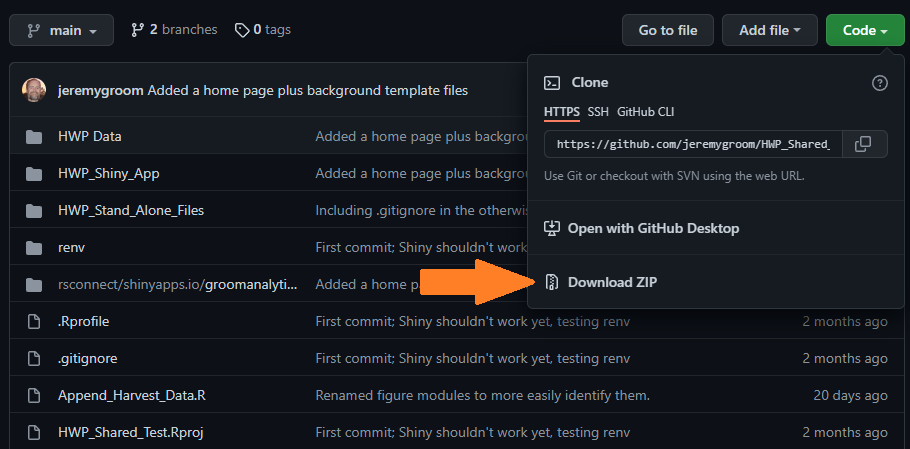
\includegraphics[width=1\linewidth]{images/zip} \caption{GitHub repository location for downloading the compressed files.}\label{fig:zip-fig}
\end{figure}

\hypertarget{dnld-git-git}{%
\subsection{Clone the GitHub repository}\label{dnld-git-git}}

To successfully clone the repository, you will need to have a program
called Git installed on your computer. It may already be installed.
There is a bit of a learning curve to getting Git up and going, as well
as connecting to GitHub through RStudio. However, there are helpful
websites that can smooth the way:

\begin{itemize}
\tightlist
\item
  \href{https://happygitwithr.com/index.html}{Happy Git and GitHub for
  the useR}\\
\item
  \href{https://cfss.uchicago.edu/setup/git-with-rstudio/}{Using Git
  within RStudio}.
\end{itemize}

If you are not already using GitHub or similar, getting
Git/GitHub/RProject set up may take an hour or two. I recommend reading
through Happy Git website carefully and following its instructions.
Going slowly is going quickly. You will also need to
\href{https://github.com/signup?ref_cta=Sign+up\&ref_loc=header+logged+out\&ref_page=\%2F\&source=header-home}{create
a GitHub account}.

Once you have Git set up on your machine and have verified that it is
doing what you want you are ready to clone the repository. The following
is based on Chapter 16 in Happy Git and Github (specifically 16.2), and
assumes that your RStudio can connect to GitHub:\\
1. Select a location on your computer where you would like a folder
containing the code to be placed.\\
2. Start R studio.\\
3. Select the following menu options: File \textgreater{} New Project
\textgreater{} Version Control \textgreater{} Git\\
4. In the ``repository URL'' paste the URL of the HWP model's GitHub
repository: \url{https://github.com/jeremygroom/HWP-C-vR.git}\\
This will automatically populate the blank below the URL with the
project name (HWP-C-vR).\\
5. Click ``Create Project''

RStudio will now open the HWP-C-vR.Rproj file for you. You are ready to
run the code. But first, we describe the files you've downloaded.

\hypertarget{dnld-files}{%
\section{File structure}\label{dnld-files}}

\emph{/HWP-C-vR/}\\
This folder contains all files associated with the model, including
template data, the Shiny application, the stand-alone code and folders,
R environment controls, and the RStudio project that runs it all.

HWP-C-vR.Rproj: Open this to operate the Shiny app or stand-alone from
your computer.

app.r: This is the main code file that runs the Shiny application.

HWP\_Stand\_Alone\_Code.R: This is the main code file for running the
stand-alone HWP model.

Append\_Harvest\_Data.R: This code will append new harvest data to your
existing data file.

README.md: This file may contain some information about the GitHub
version.

renv.loc: R environment information.

\emph{/HWP-C-vR/HWP Data/}\\
This folder contains Oregon, California, and Washington data that may be
uploaded into the app, test data for exploring the model's
functionality, and templates for constructing input files for elsewhere
in the United States.

\emph{/HWP-C-vR/HWP Data/ExistingData/}\\
This folder contains data files that may be loaded into the app or into
the stand-alone model. The files include a harvest time series and
timber and primary product ratios developed for these state-level
inventories

\begin{itemize}
\item
  CA\_Inputs\_HWP\_Model.xlsx, Oregon\_Inputs\_HWP\_Model.xlsx: These
  file contains the California and Oregon data already loaded in the
  app.
\item
  WA\_Inputs\_HWP\_Model.xlsx: This file contains data for Washington
  State.
\end{itemize}

\emph{/HWP-C-vR/HWP Data/ModelExploration/}\\
This folder contains files that allow the user to experience the app
under different data scenarios (e.g., no ownership data) and practice
appending additional data to existing files.

\begin{itemize}
\item
  bogus.xlsx: This file will cause the QA check to halt the processing
  of the data and produce a warning.
\item
  CA\_DiscardEnergyCapture\_Test: This file contains the California
  data. The worksheet for discard fates (Section
  @ref(own-prov-input-discFates)) is altered from 1980 and beyond to
  include a fraction of Discard Energy Capture (DEC).
\item
  OR\_no\_owner.xlsx: This file contains only total data for Oregon and
  lacks any ownership information.
\item
  Oregon\_MBF\_2019.xlsx: This file is not an input file. It contains
  two rows of additional Oregon harvest data for 2018 and 2019. Users
  may practice appending this harvest data to the current Oregon harvest
  data (1906 - 2017) with provided code (Section @ref(dnld-add)).
\item
  Oregon\_MBF\_2019v2.xlsx: Same as above, but this version includes all
  available Oregon harvest data (1906 - 2019).
\end{itemize}

\emph{/HWP-C-vR/HWP Data/Templates/}\\
This folder contains sub-folders that direct users to Excel templates
that they can use when building their input file.

\emph{/HWP-C-vR/HWP Data/HWP Data.zip/}\\
This file contains compressed versions of the ExistingData and Templates
folders for user download from the app.

\emph{HWP\_Shiny\_App/www/}\\
This file only contains the Groom Analytics LLC logo for the
application.

\emph{HWP\_Shiny\_App/R\_code\_data/}\\
Most of the code that the Shiny application and stand-alone HWP model
depend upon is in this folder:

\begin{itemize}
\item
  dl\_module.R: Shiny module that allows figures to be downloaded.
\item
  global.r: Initial code for reading in data for the Shiny application.
\item
  HWP.CA.output.rds, HWP.OR.output.rds: prepared data files that the
  Shiny application automatically imports to populate its figures.
\item
  HWP\_Model\_Function.r: This is the raw code for the HWP model, as is
  run by the stand-alone and the Shiny application. Note that simplified
  versions of this code are used for the Sankey diagram (located in
  PlotFunctions1.r) and the Monte Carlo simulation (see MC\_Code.R).
\item
  HWP\_Model\_Prep.R: Code that extracts values from imported data and
  prepares them for entry into the HWP model functions.
\item
  HWP\_Output\_Prep.R: Code that simplifies variable names from HWP
  model function output.
\item
  HWP\_Tables\_Code.R: Generates output tables (CSV files) that the user
  can use to recreate plots. The Shiny application has a button that
  will appear on the Upload Data selection that allows users to download
  the tables. The stand-alone code also uses this code to populate its
  own folder for tables (see below).
\item
  LakePic\_MC2.png, ShrubPic3.png: Pretty pictures for populating figure
  space when user data are not available.
\item
  MC\_Code.R: This code runs the Monte Carlo simulation using user data.
  It is used by the Shiny application and the stand-alone model.
\item
  ModelRunPage.R: This module produces the Upload Data page for the
  Shiny application.
\item
  Plot modules. Each of these provides the code to run individual Shiny
  figure tabs:

  \begin{itemize}
  \tightlist
  \item
    Plot\_AnNetChCStor\_Module.R: Produces the Annual Net Change in
    Carbon Storage tab underneath the header Carbon Storage and
    Emissions.\\
  \item
    Plot\_AnnTimHarvest\_Module.R: Produces the Annual Timber Harvest
    tab underneath the header Timber Harvest Summaries.\\
  \item
    Plot\_CStorEm\_Module.R: Produces the Carbon Storage and Emissions
    tab underneath the header Carbon Storage and Emissions.\\
  \item
    Plot\_CStorOwn\_Module.R: Produces the Carbon Storage by Ownership
    tab underneath the header Carbon Storage and Emissions.\\
  \item
    Plot\_FateHarvC\_Module.R: Produces the Fate of Harvested Carbon tab
    underneath the header Timber Harvest Summaries.\\
  \item
    Plot\_MCest\_Module.R: Produces the Monte Carlo Estimates tab
    underneath the header Carbon Storage and Emissions.\\
  \item
    Plot\_HarvFuncLS\_Module.R: Produces the Harvest by Functional
    Lifespan tab underneath the header Timber Harvest Summaries.
  \end{itemize}
\item
  PlotFunctions1.r: This code contains many of the functions used
  repeatedly by figures and the HWP model variants (standard HWP, Monte
  Carlo, and Sankey). It also contains the Sankey HWP model function.
  This code is source by the Shiny application and the stand-alone
  model.
\item
  QA\_Code\_Shiny.r: This code runs a Quality Assurance procedure on
  imported data. It verifies that the data are formatted correctly for
  entry into the HWP and Monte Carlo models. For more detail on the
  quality assurance procedure, see Section @ref(own-qa).
\end{itemize}

\emph{/HWP\_Stand\_Alone\_Files/Arrays/}\\
This folder serves as a destination for the arrays generated by the
stand-alone code, given that the user's data file indicates that arrays
should be generated. The .gitignore file prevents the source code from
uploading the arrays to GitHub.

\emph{/HWP\_Stand\_Alone\_Files/QAQC\_Reports/}\\
This folder contains the error report (Error\_Report.csv) generated by
the stand-alone code's call to QA\_Code\_Shiny.r. The .gitignore file
prevents the source code from uploading any error reports in this folder
to GitHub.

\emph{/HWP\_Stand\_Alone\_Files/Standalone\_R\_files/}\\
This folder contains two code files, MC\_Tables.R and Sankey\_Code.r. If
the user indicates that the stand-alone code should generate tables of
the Monte Carlo outcome, the MC\_Tables.R file generates the tables. If
the user indicates that the stand-alone code should generate a Sankey
figure the Sankey\_Code.r file will do so.

\emph{/HWP\_Stand\_Alone\_Files/Tables/}\\
This folder serves as a destination for tables generated by the
stand-alone code, given that the user's data file indicates that arrays
should be generated. The tables are the same as those generated by the
Shiny application after the user has run the HWP model on their own data
and then selected the button that generates the tables. The .gitignore
file prevents the source code from uploading any tables in the folder to
GitHub.

\emph{/renv/}\\
This folder contains R environment variables that the Shiny application
(app.r) and stand-alone model (HWP\_Stand\_Alone\_Code.R) rely upon. The
environmental variables include version information for R and the
libraries used. The user can ignore this folder.

\emph{/rsconnect/}\\
This folder contains shinyapps.io deployment information. The user can
ignore this folder.

\hypertarget{dnld-shiny}{%
\section{Running the Shiny app from your computer}\label{dnld-shiny}}

\begin{enumerate}
\def\labelenumi{\arabic{enumi}.}
\item
  Open the code in RStudio. Launch the RStudio project by opening the
  project file \textbf{HWP-C-vR.Rproj} from within its folder. Within
  RStudio select from the menu File \textgreater{} Open File\ldots{} .
  Select the file \textbf{app.r} and click on the Open button.
\item
  Run the code in RStudio. Here we run all of the code in the
  \textbf{app.r} file. There are several ways to do this. One way is to
  click on the code itself inside the code window, select all of the
  code (ctrl+A on a PC, apple+A on a Mac), and then ctrl+Enter (or
  apple+Enter) to run everything. Or, go to the menu item and select
  Code \textgreater{} Source.
\end{enumerate}

Once you have run the Shiny application code, RStudio will display the
application in its own window. A button at the top of the window will
allow you to open the application in your own browser, but this isn't
necessary. The application should function as it does online when run
from the Shinyapps.io server.

\hypertarget{dnld-shiny-details}{%
\subsection{Details on running and editing the
code}\label{dnld-shiny-details}}

Users can run one or more lines of code by highlighting them and
pressing ctrl-Enter or apple-Enter, or from the RStudio menu selecting
Code \textgreater{} Run Selected Line(s).

The first line of the app.r or HWP\_Stand\_Alone\_Code.R is:
\texttt{renv::restore()}. The first time you run this line on its own or
when running all of the code, the project file will (with your
permission) download all versions of all libraries and the R instance
used to run the app (\protect\hyperlink{ref-R-renv}{Ushey 2022}). It
takes a little while, but you'll only need to do it once. This version
control step hopefully helps prevent conflicts between your newer or
older versions of previously-installed R libraries and the code.

The stand-alone code relies heavily upon functions and code chunks
located in the Shiny app code folder (HWP\_Shiny\_app/R\_code\_data/).
Updates to these code files can affect both the app and stand-alone
code. For instance, the guts of the HWP model are in the file
HWP\_Model\_Function.r, which both the Shiny app and the stand-alone
code rely upon.

The user can alter the Shiny code to produce different figures or to
extract intermediary or final data frames used for figure generation. As
a warning, if the user alterations cause an error, the Shiny application
can break. Troubleshooting in a Shiny application is not as
straightforward as it is in standard R code (In the online book
\href{https://mastering-shiny.org/index.html}{Mastering Shiny} by
Wickham (\protect\hyperlink{ref-wickham2021}{2021}), see
\href{https://mastering-shiny.org/action-workflow.html}{Chapter 5
Section 2, Debugging}). I will not discuss the workings of Shiny to any
extent here (if interested, see the previous link for more information),
but if the user inserts the code \texttt{browser()} immediately after an
item of interest, saves the change to the code, re-runs the Shiny app
from their computer, and selects the figure or item of interest from the
application, the code will halt at the \texttt{browser()} call and the
user can inspect all elements created to that point.

\hypertarget{dnld-sa}{%
\section{The Stand-alone model: benefits, utility, and how to
operate}\label{dnld-sa}}

The stand-alone model provides the user with little additional utility
over the web-based Shiny application. It will produce arrays used by the
model, and these can be useful for reconstructing analysis results and
understanding how the model operates. It can also produce the Sankey
diagram, showing the flow of harvested carbon from a single year to
various storage and emission pools at various points in time, but within
RStudio. The RStudio Plots window has an Export option that will save
the Sankey figure as a PNG file, an option that the Shiny application
cannot provide. However, the PNG resolution is not much greater than a
screen shot of the Sankey diagram from the web application. The PNG
version also does not reflect any manipulation of the figure by the user
after the figure was produced (e.g., if the user slides the categories
around to better separate them, the PNG will only show the figure as
initially produced).

The main advantage of the stand-alone model code is that the user can
step through it line by line to better understand what the code is
doing. The code is arranged in a much more readable way than it is for
the Shiny application. The user can step through the code piece wise or
run all of the code at once after placing their data file in the HWP
Data folder and entering their file name into the code as described
below.

To run the stand-alone code, open the file ``HWP-C-vR.Rproj''. This will
open the R Project using the program R Studio. Open the file
``HWP\_Stand\_Alone\_Code.R''. Then, run the \texttt{renv::restore()}
line plus the library load code. If this is the first time you are
running the \texttt{renv::restore()} call, the process may take a few
minutes to complete.

The next few lines select whether you wish to generate the Sankey
diagram, which year you would like to generate it for, and for how many
years the decay process should be run. Change
\texttt{GENERATE.SANKEY\ =\ TRUE} to \texttt{GENERATE.SANKEY\ =\ FALSE}
if you do not wish to generate the Sankey diagram. Change the year in
\texttt{SANKEY.HARVEST.YEAR} and \texttt{SANKEY.YEARS.OF.HARVEST} to
your year of interest and the number of years of decay, respectively. It
would probably be most efficient to figure out these years/decay times
beforehand by using the Shiny application.

The \texttt{\#\#\#\ Folder\ locations} lines should mostly remain
unchanged unless you would like to move files about for some reason. The
\texttt{IMPORT.DATA.FOLDER} will change depending on whether you wish to
access existing input files, altered template data, or any input files
you have saved elsewhere. The \texttt{IMPORT.DATA.FILE} value should be
changed to the file name that you would like to import. Be sure your
file is in the HWP Data folder (unless you've redefined the
\texttt{IMPORT.DATA.FOLDER} location accordingly). Run these lines.

Run the lines for loading the data, including those for the QA test
(approximately lines 50 through 85). The code, given your file name,
will open your file and extract worksheets. If the user data prescribes
that the QA test to be run, this code will source the QA\_Code\_Shiny.r
file. Otherwise, it will skip the QA test and load the files
automatically. The QA test takes little computation time, so omitting
this step does not speed up the code greatly.

Run lines 90 -- 111. These lines source code that prepares the data for
entry into the model and extracts certain options from the user data,
like whether to save tables and arrays, and the locations where they
should be saved. The code also sources the PlotFunctions1.r code to
obtain some functions used by the HWP model, and the HWP model function
itself.

Running lines 112 -- 128 causes the code to run the HWP model and
extract the model function's outputs.

Running lines 130 -- 148 enact a year-shift in the data if the user
wishes. The year-shift causes all fates from harvest (waste from
processing, placement of carbon in products in use, etc.) to occur the
year after harvest, as in the original USFS versions of the model.

Running lines 150 -- 164 will generate table CSV files in the Tables
folder if the user's data defines \texttt{OUTPUT\_TABLES} to be
\texttt{TRUE}. Otherwise the code is skipped.

Lines 165 -- 200 will generate array Excel files in the Arrays folder if
the user's data defines \texttt{OUTPUT\_ARRAYS} to be \texttt{TRUE}.
Otherwise the code is skipped. Note that array generation does take some
noticeable time; it may be useful to set this option in the data to
FALSE when running the overall code set frequently.

Lines 200 -- 210 cause the Monte Carlo to run. The Monte Carlo can be
very time-consuming to run. Consider setting the data option to
\texttt{FALSE} if only outputs from the regular HWP model are needed.

Lines 211 -- 220 run the Sankey code if the user selected for the
generation of the Sankey diagram to take place (\texttt{TRUE}).

\hypertarget{dnld-sa-arrays}{%
\subsubsection{Generated array files}\label{dnld-sa-arrays}}

If the user's data input file indicates that the stand-alone model code
should generate arrays (Section @ref(own-prov-input-options)), the
arrays will be deposited in the folder HWP\_Stand\_Alone\_Files/Arrays/.
The arrays all occur and operate within the file
\textbf{HWP\_Model\_Functions.r} and have the dimensions of rows = EUR
categories, columns = years, workbook tabs = ownerships. The following
arrays will be generated, with their working names that may be found in
the schematics of Section @ref(model-func-schem):

\begin{itemize}
\item
  \textbf{bwoec\_array.xlsx} - Working name in the code:
  bwoec.input\_array. This is the amount of all discarded material (see
  dp.total\_array.xlsx) that is burned without energy capture.
\item
  \textbf{compost\_array.xlsx} - Working name in the code:
  compost.input\_array. This is the amount of all discarded material
  (see dp.total\_array.xlsx) that is composted.
\item
  \textbf{dec\_array.xlsx} - Working name in the code: dec.input\_array.
  This is the amount of all discarded material (see
  dp.total\_array.xlsx) that is burned with energy capture.
\item
  \textbf{dp.total\_array.xlsx} - Working name in the code:
  dp.total\_array. The amount of carbon discarded each year. This
  includes byproduct of harvested wood products (see PIU.WOOD.LOSS and
  PIU.PAPER.LOSS, Section @ref(own-prov-input-options)) and the annual
  amount of products in use that become discarded material.
\item
  \textbf{dumps.discard\_array.xlsx} - Working name in the code:
  dumps.discard\_array. The amount of carbon in dumps each year that
  decays.
\item
  \textbf{dumps\_array.xlsx} - Working name in the code: dumps\_array.
  The amount of carbon residing in dumps.
\item
  \textbf{eec\_array.xlsx} - Working name in the code: eec\_array. The
  amount of carbon that is emitted with energy capture each year. This
  consists of carbon directly burned as fuel (fuel\_array.xlsx) and
  discarded carbon that is burned for energy (dec\_array.xlsx).
\item
  \textbf{eu.reduced\_array.xlsx} - Working name in the code:
  eu.reduced\_array. This array contains all carbon in Tg C serving as
  input to the model after the ``products in use'' loss occurs.
\item
  \textbf{eu\_array.xlsx} - Working name in the code: eu\_array. This
  array contains all carbon in Tg C serving as input to the model.
\item
  \textbf{ewoec\_array.xlsx} - Working name in the code: ewoec\_array.
  This is the amount of all discarded material (see
  dp.total\_array.xlsx) that is burned without energy capture.
\item
  \textbf{fuel\_array.xlsx} - Working name in the code: fuel\_array. The
  amount of harvested wood products that directly serves as fuel.
\item
  \textbf{lf.decaying\_array.xlsx} - Working name in the code:
  landfill\_array. This is the amount of discarded products that resides
  in the portion of landfills that is subject to decay.
\item
  \textbf{lf.discard\_array.xlsx} - Working name in the code:
  landfill.discard\_array. This array captures the quantity of the
  decaying landfill that decays each year.
\item
  \textbf{lf.fixed.cumsum\_array.xlsx} - Working name in the code:
  lf.fixed.cumsum\_array. The cumulative sum across years of the amount
  of carbon in the non-decaying portion of landfills.
\item
  \textbf{lf.fixed.input\_array.xlsx} - Working name in the code:
  lf.fixed\_array. The amount of discarded products that is sent to the
  non-decaying portion of landfills each year.
\item
  \textbf{pu.final\_array.xlsx} - Working name in the code:
  pu.final\_array. This is the total amount of carbon in Products in
  Use, including recovered (recycled) products (recov\_array.xlsx) + and
  the not-yet-recovered Products in Use pool (pu\_array.xlsx).
\item
  \textbf{pu\_array.xlsx} - Working name in the code: pu\_array. This is
  the pool of carbon in Products in Use. It is subject to decay.
\item
  \textbf{recov.discard\_array.xlsx} - Working name in the code:
  recov.discard\_array. This array captures the quantity of recovered
  material that decays each year.
\item
  \textbf{recov\_array.xlsx} - Working name in the code:
  recov.input\_array. This is the amount of all discarded material (see
  dp.total\_array.xlsx) that is recovered (recycled).
\item
  \textbf{swds.total\_array.xlsx} - Working name in the code:
  swdsCtotal\_array. Total amount of carbon in solid waste disposal
  sites. This is the amount of carbon residing in the non-decaying
  portion of landfills (lf.fixed.cumsum\_array.xlsx) + carbon in the
  decaying portion of landfills (landfill\_array.xlsx) and in dumps
  (dumps\_array.xlsx)
\end{itemize}

\hypertarget{dnld-add}{%
\section{How to add new data years to your data set}\label{dnld-add}}

Users may wish to generate model outputs annually or every few years
with new harvest values. However, they may not want to alter all of the
worksheets in their data file by hand to account for the newly added
harvest years. The file \textbf{Append\_Harvest\_Data.R} takes, as
input, an Excel file with a single worksheet of harvest by thousand
board feet, formatted in the same way as their earlier Harvest\_MBF
worksheet. The user points the code toward their original data file, the
new Harvest\_MBF Excel file, and provides a name for the output Excel
file. They also provide a location for the new file to be written. The
code will make all necessary changes to the original file and append the
new years. Importantly, where needed, the code will read values used for
the year prior and duplicate them in the new data set. Therefore, if the
user wishes to update Timber Product Ratios, Primary Product Ratios, End
Use Ratios, or any other dataset, they will need to do so by hand,
possibly after this procedure is run.

As an example, say we wish to add 2018 and 2019 harvest levels to
Oregon's data. We open the Append\_Harvest\_Data.R file in the
\texttt{HWP-C-vR.Rproj} RStudio project, run the first few lines that
load the needed libraries, and then alter the following lines to read:

\texttt{ORIG.DATA.FILE\ \textless{}-\ "Oregon\_Inputs\_HWP\_Model.xlsx"}\strut \\
\texttt{NEW.DATA.FILE\ \textless{}-\ "Oregon\_MBF\_2019.xlsx"}\strut \\
\texttt{OUT.DATA.FILE\ \textless{}-\ "Oregon\_Inputs\_HWP\_Modelv2.xlsx"}

\texttt{ORIG.DATA.FOLDER\ \textless{}-\ "HWP\ Data/ExistingData/"}\strut \\
\texttt{NEW.DATA.FOLDER\ \textless{}-\ "HWP\ Data/ModelExploration/"}\strut \\
\texttt{OUT.DATA.FOLDER\ \textless{}-\ "HWP\ Data/ModelExploration/"}

The first of those lines identifies the name of the original data, the
second the name of the file with the Harvest\_MBF data for the new
years, and the third line assigns the name of the output data file.
Lines 4-6 identify the folder locations of the original, updated, and
output data set Excel files.

The new data file can provide data for just the new years (e.g.,
\texttt{Oregon\_MBF\_2019.xlsx}); or, the user can provide all of the
original harvest data in addition to the more recent harvest data (e.g.,
\texttt{Oregon\_MBF\_2019v2.xlsx}). Once those six lines are correct the
user can select and run all of the code from the file. The code will
attempt to generate a new Excel file with the desired updates. The code
also performs some QA checks:

\begin{itemize}
\item
  Verifies that data are numeric
\item
  Verifies that the original and new data do not duplicate or skip years
\item
  If ownership data are present in the original data, the code verifies
  that ownership data exist in the new data too, and that the Total
  column equals the sum of other ownership columns.
\end{itemize}

The code will print error messages if any of those tests are not passed.

If errors are encountered and the files are altered to correct those
errors, be sure to close the newly generated file before running the
code again. Otherwise, R will generate an error message.

\hypertarget{model}{%
\chapter{HWP Model Operations}\label{model}}

\hypertarget{model-func}{%
\section{HWP model function}\label{model-func}}

\hypertarget{model-func-inp}{%
\subsection{Model inputs}\label{model-func-inp}}

The HWP model is a deterministic model which relies on optional and
required user-supplied information. The user must supply annual timber
harvest volumes in board feet (MBF) by ownership, annual timber product
ratios (TPR) that allocate harvest to different timber product classes,
annual primary product ratios (PPR) that allocate timber products to
different primary products and residue uses, and annual end-use product
ratios (EUR) which are subcategories of PPR that represent the final
products produced.

The user may, at a minimum, provide timber harvest volumes and then rely
on default California and Oregon values. These include a board foot to
cubic foot conversion factors for sets of years and conversion factors
between hundred cubic feet (CCF) and metric tons of carbon (MT C) or
teragrams of carbon (Tg C) for the primary products. The model uses
end-use half-life values to determine how long carbon resides in
Products in Use (PIU) before becoming discarded.

The user may also provide ratios for discard fates. These ratios
determine, by year, what fraction of discarded paper and wood are
channeled into one of six discard categories: burned (Emitted without
Energy Capture, EWOEC), discard energy capture (DEC), composted, sent to
a dump, enter the non-decaying portion of a landfill, or become landfill
subject to decay. Users may also adjust half-life values for paper and
wood discards in landfills and dumps and the fraction of material
entering landfills that is subject to decay or remains permanently.

\hypertarget{model-func-opp}{%
\subsection{Summary of model operations}\label{model-func-opp}}

In the next section we provide a detailed schematic of how the HWP model
code operates. A more general schematic of the process, very similar to
Figure 7 in Stockmann et al.
(\protect\hyperlink{ref-stockmann2012}{2012}), is presented in Figure
@ref(fig:overview-fig). Here we provide a written description of the
code's actions. We start out with data sets and variable information
that are arranged by different combinations of year, ownership, and
ratio types. First the code converts harvest data in units of MBF to CCF
using BF to CF conversion ratios and other standard unit conversion
factors. The model combines Primary Product Ratios (PPR) with Timber
Product Ratios (TPR) and then joins those with the timber harvest volume
in CCF by year. These are then joined with conversion values for CCF to
metric tons of carbon, and the End Use Ratios (EUR). The result is a
data set called eu\_ratios, and values for EUR, TPR, PPR, the harvest
amount, and the CCF to metric tons of carbon conversion factor are
multiplied together to produce a variable called MTC for Metric Tons of
Carbon. One million MTC (MMT C) = one Tg C. This variable serves as the
carbon input into the model and has the correct units of carbon input
per year for each EUR category.

For each year, some of the carbon, fuel wood, is immediately burned and
is Emitted with Energy Capture (EEC). A certain percentage (8\% for
California and Oregon data) of the carbon allocated to each of the
remaining EUR categories is discarded and enters the Discarded Products
process and the remaining 92\% become the annual carbon addition to the
Products in Use (PIU) process. The provided data input and template
files by default assume that 100\% of pulp wood becomes paper with no
loss. However, users may adjust this percentage if they wish (Section
@ref(own-prov-input-options)).

The Products in Use process calculates, for every year, the amount of
carbon remaining from the year prior and the amount of carbon entering
the process as new PIU. A decay function considers the previous year's
carbon amounts in each EUR/ownership category, applies a decay
calculation, adds the result to the amount of incoming PIU carbon, and
saves the value as the amount of PIU carbon for that year. It also
records the amount of carbon that was discarded from the process and
sends that carbon to the Discarded Products process.

The Discarded Products process uses proportions to divide incoming
discarded products among six fates: burn without energy capture, burn
with energy capture, compost, dump, landfill, and recovered (recycled).
Burned without energy capture and composted proportions are treated as
EWOEC. The proportion of discarded products that are burned for energy
capture (DEC) will be treated as EEC (for California and Oregon all
carbon is currently modeled as BWOEC). Discarded Products that are
recovered or sent to dumps are processed with the same decay function
used for Products in Use, but with different half-life values. Decay
from recovered products does not re-enter the Discarded Products process
but instead is treated as EWOEC. The outputs that do not decay in a
given year are treated either as Products in Use (recovered) or Solid
Waste Disposal Site (SWDS) material (dumps). Discarded Products that are
sent to Landfill are treated like Dumps, except that a proportion of the
landfill is not subject to decay. That amount will become one of the
carbon pools that comprise SWDS. The remainder of carbon in the landfill
decays and is treated as EWOEC or remains in the landfill and is counted
as another SWDS carbon pool: landfill material subject to decay.

The HWP code's outputs are EEC and combined versions of EWOEC, PIU, and
SWDS. The final EEC values are the original EEC values for fuel wood
plus the fraction of the discarded materials that are burned with energy
capture (DEC). The final EWOEC amounts are combinations of emissions
from dumps, recovered materials, landfill decay, burnt refuse, and
compost materials. PIU is the combination of the original PIU values
plus recovered carbon that has not decayed. SWDS is the non-decaying and
decaying carbon in landfills plus remaining carbon in dumps.

\hypertarget{model-func-schdesc}{%
\subsection{Model schematic description}\label{model-func-schdesc}}

Below we provide a schematic of how the HWP model operates. The
schematic color codes items and flows from the top to bottom of each
page. Inputs, such as worksheets from the Excel data file, are yellow.
Calculated matrices or arrays are blue. Final output, which may be
manipulated to produce tables and figures, are purple. Calculations or
data transformations are peach colored.

The file and object names listed in the schematic may be found in the
provided model code. My intent is to provide a written description
(above) that assists readers with understanding the schematic, which in
turn can be used to interpret how the R code (HWP\_Model\_Function.R)
works. The R code itself is annotated. Readers may alter the code to
incorporate their own files or improve upon the model (see Chapter
@ref(dnld)).

Transformations include database functions such as pivots and joins. A
pivot in this case usually involves lengthening a matrix by taking
several columns of data and stacking them into one column, with a second
column identifying which of the original columns they came from. This
format is useful for combining data with different levels of
information. For instance, we might have data with rows = different
ownerships and columns = years. We can pivot those data such that there
is a column of ownership, a column for the years (years will be repeated
for each block of ownerships), and a column for the values. Say we have
another pivoted data set that has data for ownership, years, and Timber
Product Ratios. We can join the two data sets by matching years and
ownership values and duplicating the data values from the first data set
across all of the Timber Product Ratios for each year/ownership
combination. A somewhat more complicated version of this example is
described in the Model Start page of the schematic.

Ultimately, the code may produce a final pivot length of well over
100,000 rows. This is equal to the number of End Use Ratio values *
number of ownerships (including a Total column) * number of years. For
instance, the eu\_ratio matrix has this many rows and several useful
variables that are used to calculate metric tons of carbon from harvest
as distributed across EURs, years, and ownerships. This value is then
placed in a three-dimensional array with row number = number of EUR
rows, depth = ownership number, and column number = number of years of
data. The HWP code frequently uses arrays of these dimensions for
storing values from many types of calculated data.

Each page of the following schematic has a title. These titles may be
referred to within the schematic, as certain program products are used
in later pages. If a calculated data set's boarders have thick black
dashes, the data set is from a previous page. If a calculated data set
lies within some white space with a thick black dashed boarder, the
white space includes information on which page that product is destined
for.

The HWP program has a decay function that is used repeatedly. The same
function operates on Products in Use and the decaying portion of
landfill, dumps, and recovered (recycled) products. As an example, for
PIU, the function iterates through years for a given ownership/EUR
combination. It calculates the amount of PIU carbon carried over from a
previous year by subjecting that carbon to its appropriate half-life
value. Then it adds that carbon to the incoming PIU carbon for that
year. Then it moves forward one year and repeats.

\newpage

\hypertarget{model-func-schem}{%
\subsection{Model Schematic}\label{model-func-schem}}

Model Dimensions Key:\\
Y = number of years (California = 68, from 1952 to 2019)\\
y = particular year\\
I = ownerships including Total (California = 6)\\
i = particular ownership\\
T = Timber product ratio number (California = 40)\\
P = Primary product ratio number (California = 64)\\
E = End use ratio number (California = 224)\\
e = particular EUR\\
piu.wood.loss = Loss percentage for wood products entering PIU
(California = 8\%)\\
piu.paper.loss = Loss percentage for paper products entering PIU
(California = 0\%)

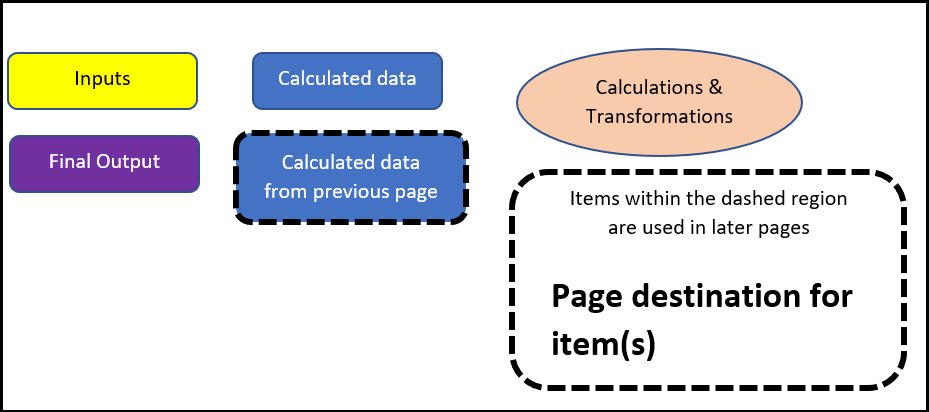
\includegraphics[width=1\linewidth]{images/schematic-0}

\newpage

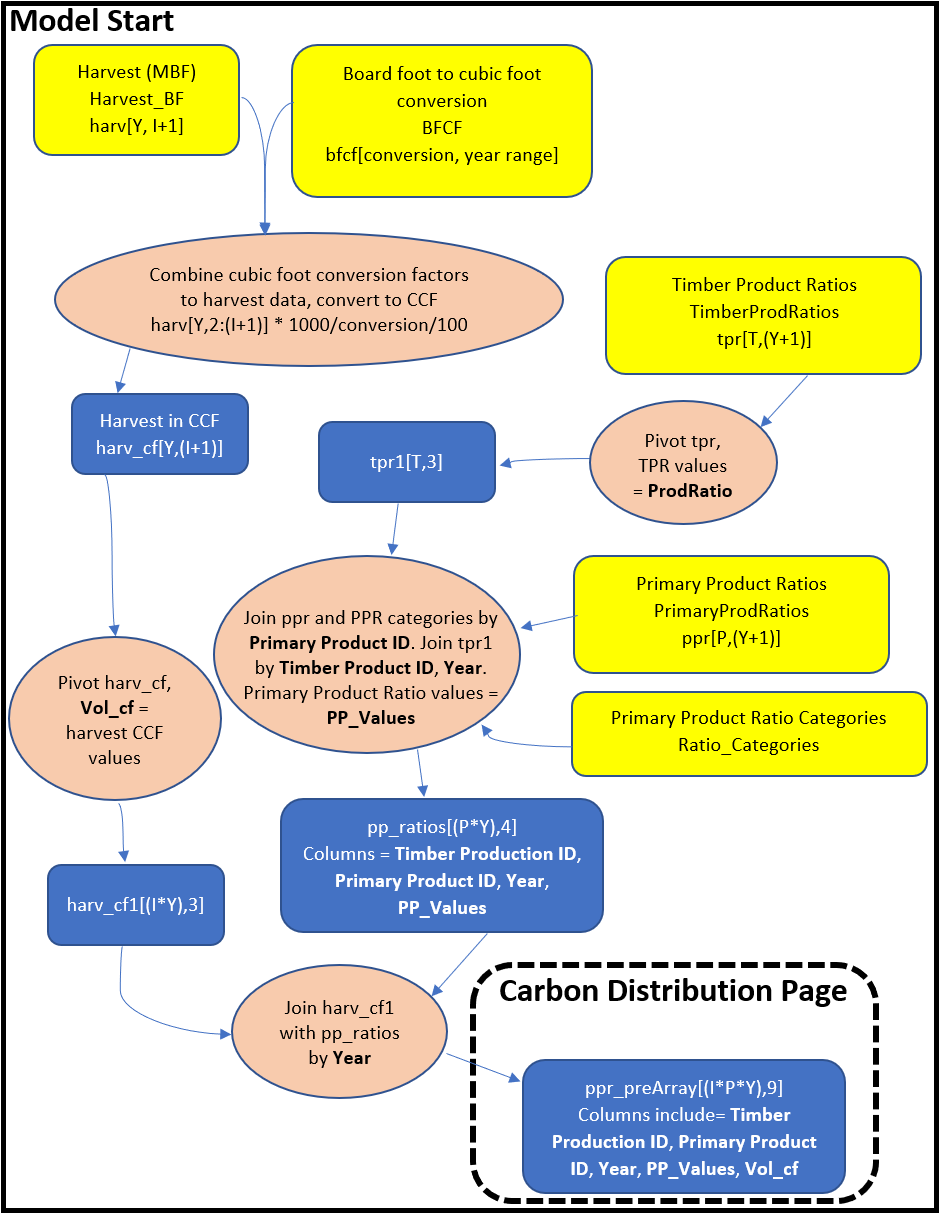
\includegraphics[width=1\linewidth]{images/schematic-1}

\newpage

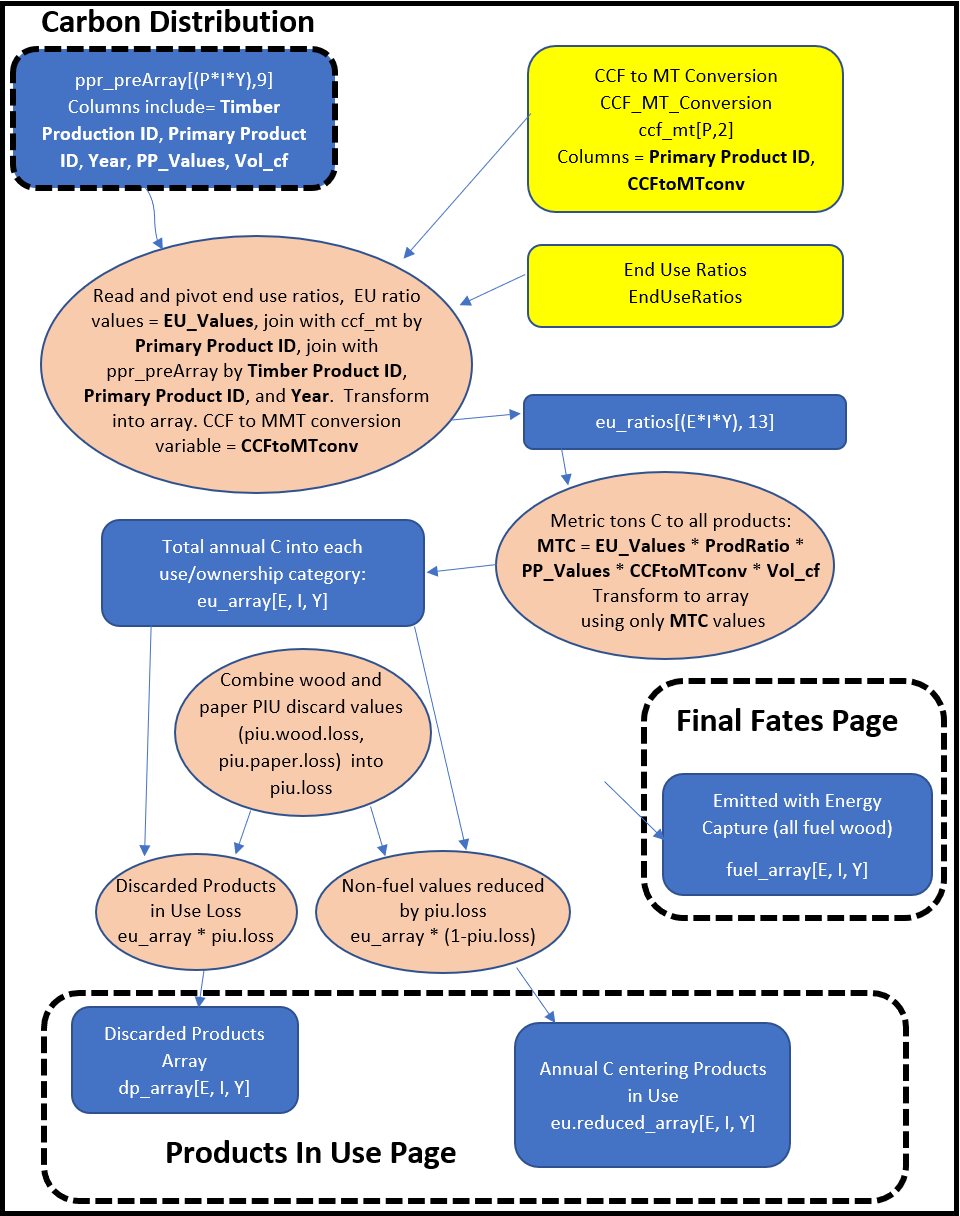
\includegraphics[width=1\linewidth]{images/schematic-2}

\newpage

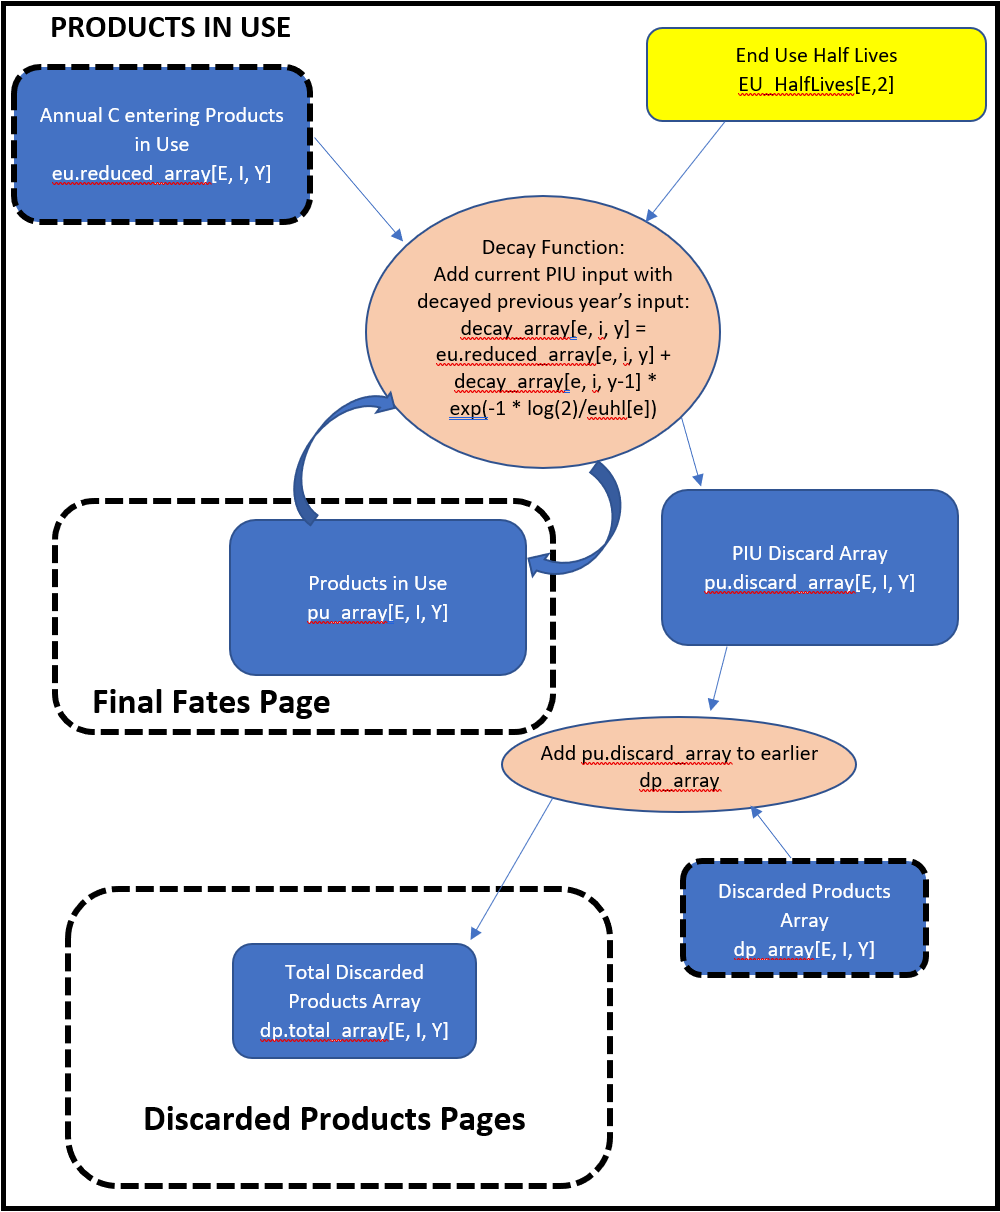
\includegraphics[width=1\linewidth]{images/schematic-3}

\newpage

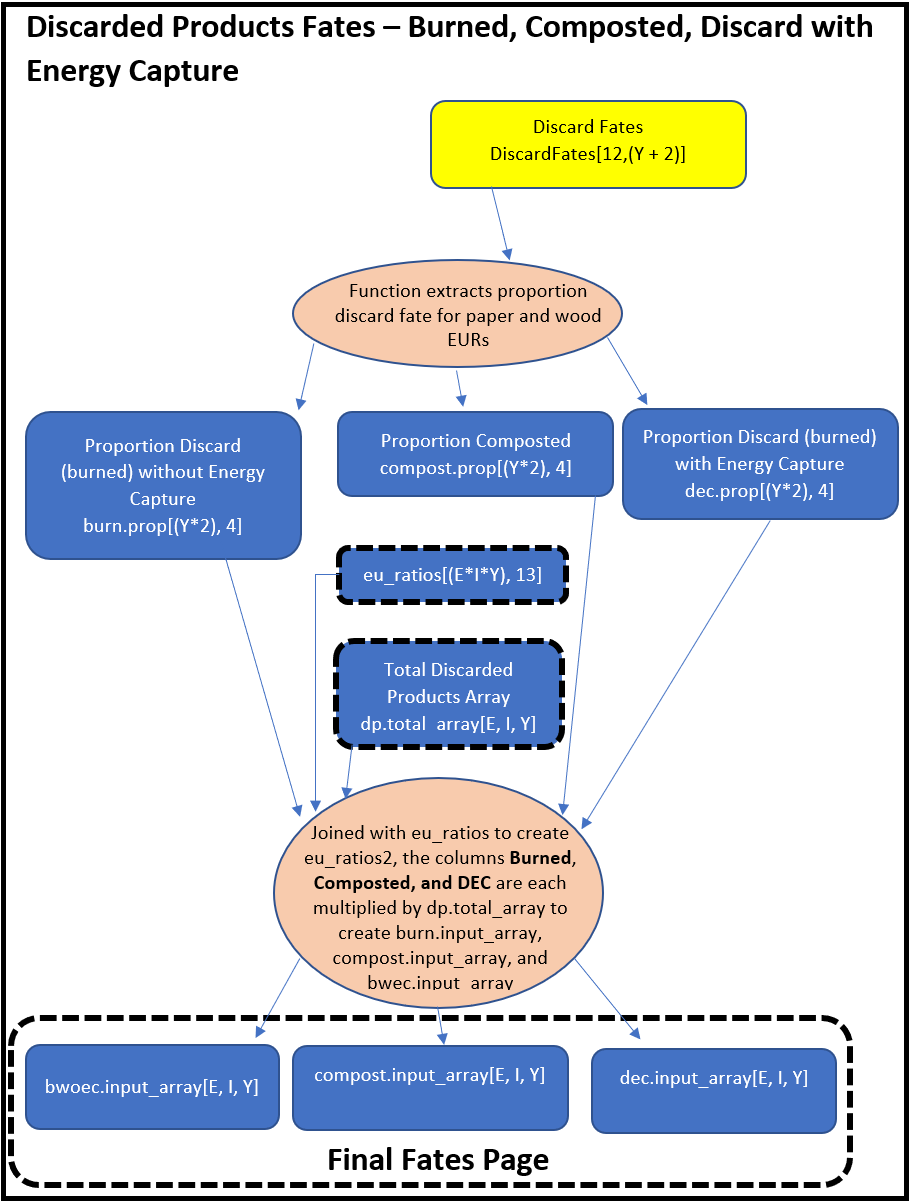
\includegraphics[width=1\linewidth]{images/schematic-4}

\newpage

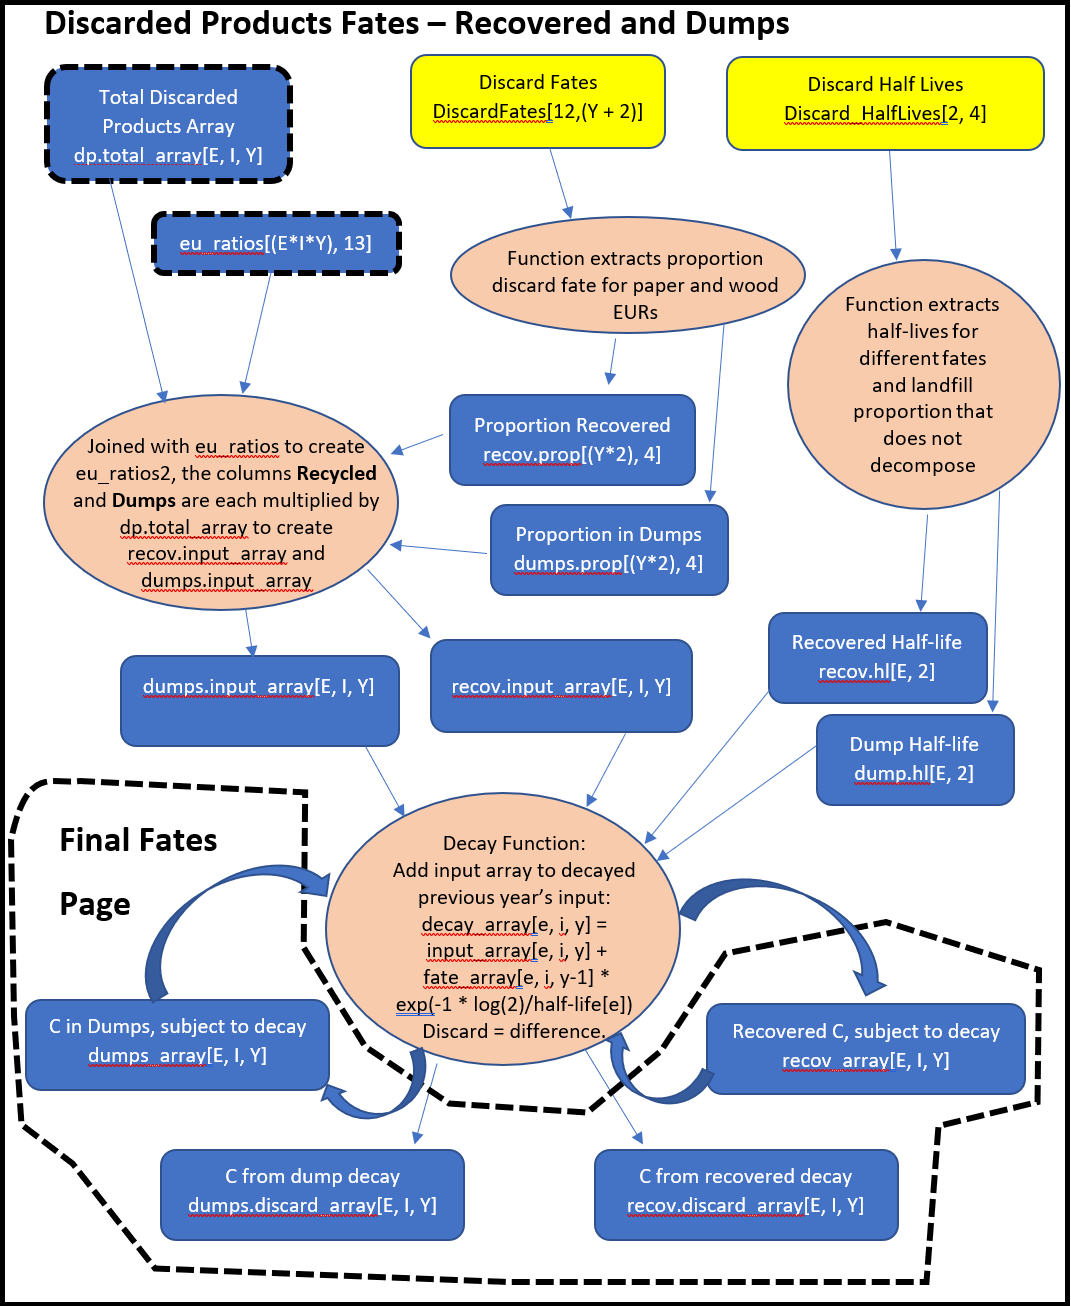
\includegraphics[width=1\linewidth]{images/schematic-5}

\newpage

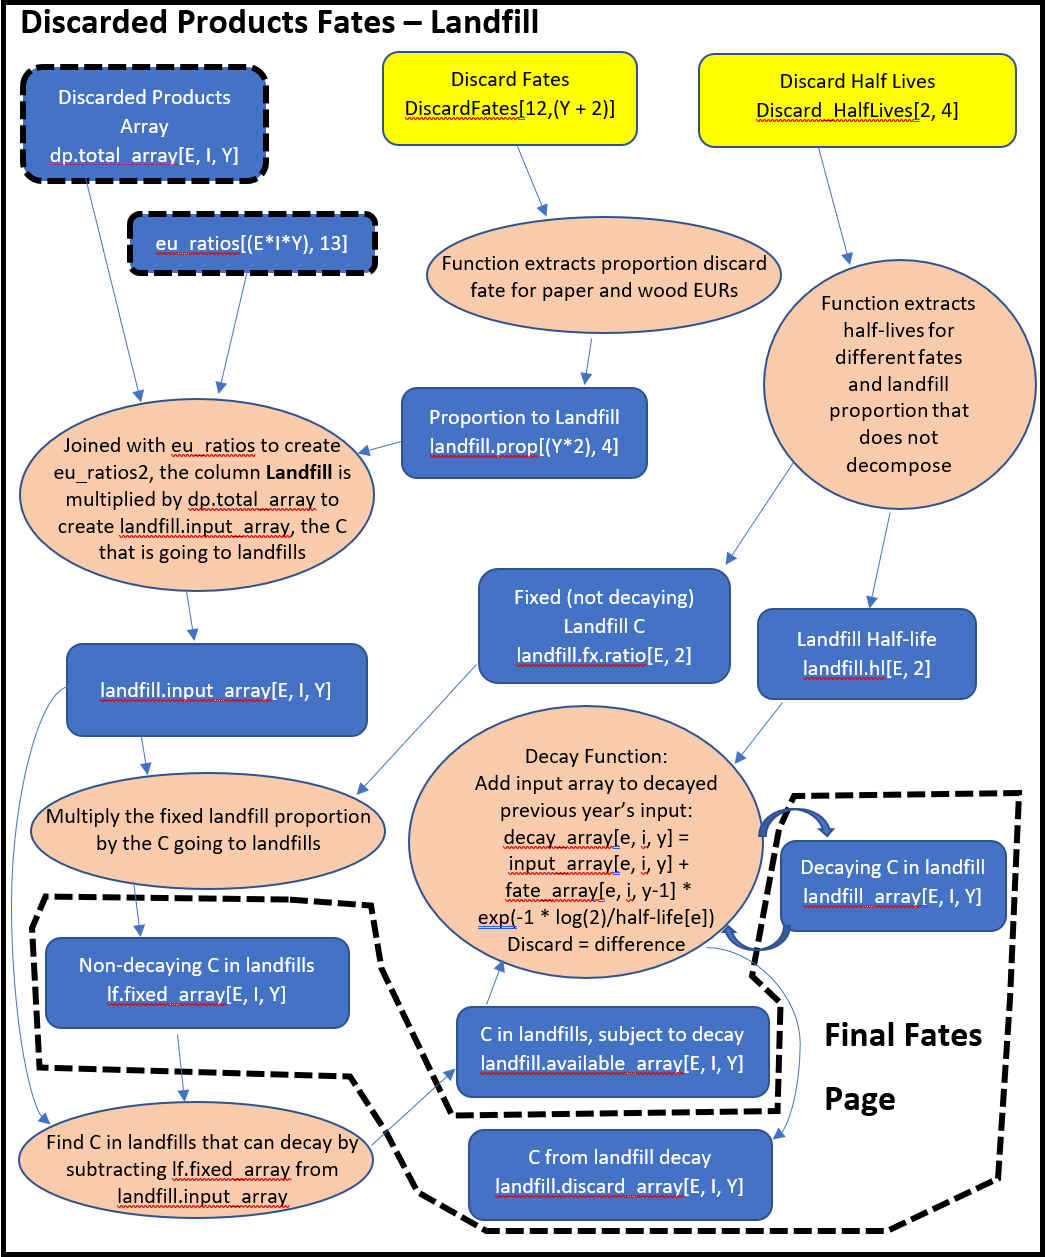
\includegraphics[width=1\linewidth]{images/schematic-6}

\newpage

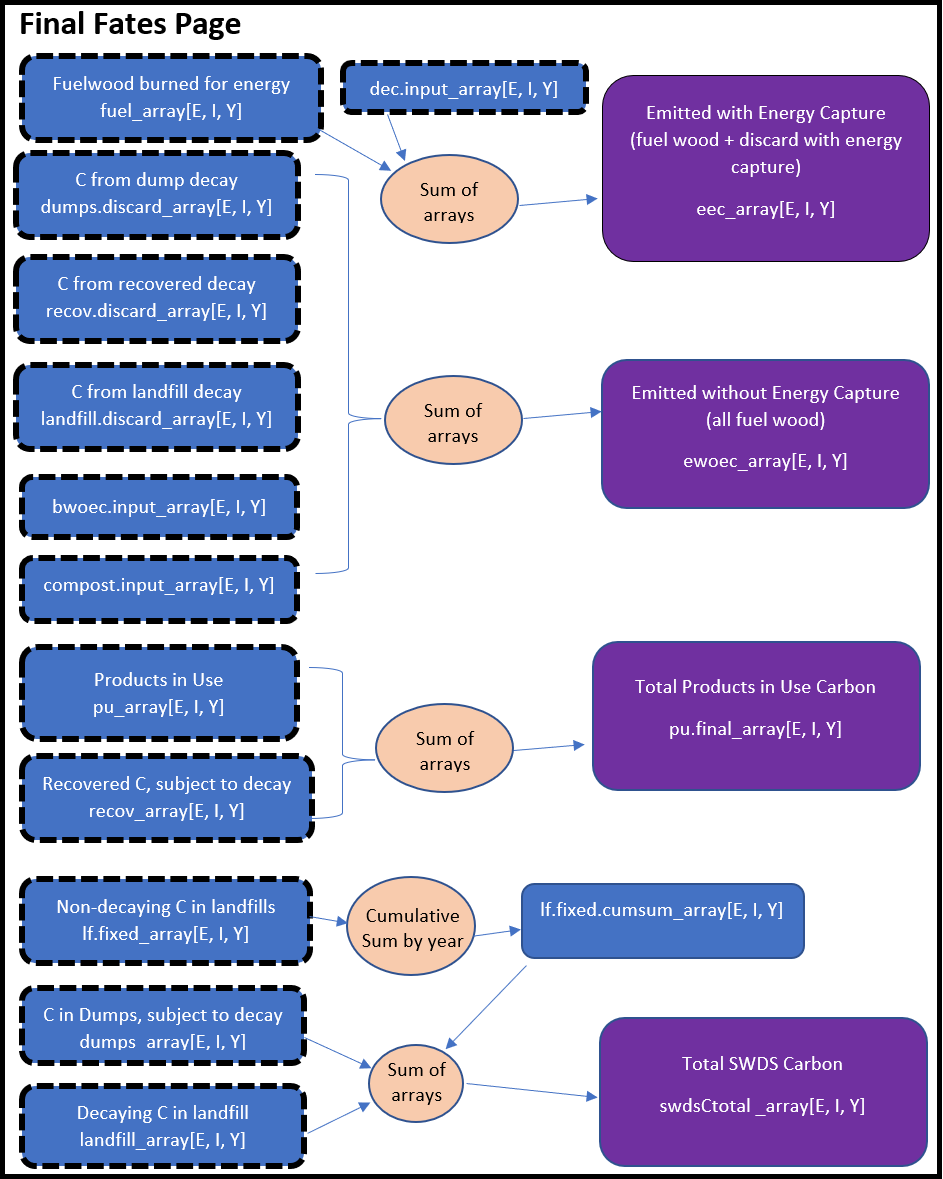
\includegraphics[width=1\linewidth]{images/schematic-7}

\hypertarget{model-func-out}{%
\subsection{Model Outputs}\label{model-func-out}}

The model described above treats timber harvest, product manufacture,
and disposal as processes that occur within the same year. To match
other reports, outputs are altered (SHIFTYEAR = TRUE; see Section
@ref(own-prov-input-options)). All trees harvested in a given year are
treated as processed within that year and the carbon is distributed
according to the end use product ratios of that same year. Most of the
carbon is immediately burned or turned into Products in Use. A fraction
(the default 8\%) is immediately discarded and distributed to the
different discard fates using the discarded disposition ratios for the
same year. The carbon fate for a given year is reported for the
following year. Carbon that enters the model in a given year does not
undergo a half-life decay until the following year. For example, the
model uses the Timber Production Output for 1906 and all product and
discard ratios for 1906 to distribute the carbon in Products in Use,
Discard Energy Capture, and the discard fates. The sum of those fates
for 1906 is recorded in tables as occurring by January 1, 1907. Any
carbon from 1906 that was distributed to Products in Use, Landfill, or
Dumps was subject to a half-life decay or disposal in 1907.

When users upload their data to the Shiny application or run the
stand-alone model, they have the opportunity to download or generate
summary tables of the model output. The provided tables should allow,
with effort, the user to reproduce all Shiny application figures except
for those associated with the Sankey diagram.

The stand-alone code can optionally save the arrays used to generate the
tables in the folder ``Arrays''. Unlike the table outputs for stocks and
emissions the arrays are not year-shifted. The arrays are provided for
results-checking and data exploration. The arrays are three dimensional
but are saved as Excel workbooks. Excel worksheet rows represent the end
use ratios, columns represent years, and each worksheet tab is an
ownership with the final tab representing the ``Total'' carbon value.
Some arrays are combinations of other arrays, described below. File
``eu\_array.xslx'' is the distribution of carbon (metric tons) to end
uses. Values are used to convey how harvested wood in each ownership
category translates to Tg C for each of the end use products. This array
is effectively the starting point for all C fates.

Users are encouraged to generate the arrays (OUTPUT\_ARRAYS = TRUE) in
the stand-alone model and verify calculations. The above flow diagram
provides array names and a general description of how they are used. The
code file HWP\_Model\_Function.r provides more detail about how they are
used.

\hypertarget{model-mc}{%
\section{Monte Carlo simulation}\label{model-mc}}

\hypertarget{model-mc-spec}{%
\subsection{Simulation specifications}\label{model-mc-spec}}

The Monte Carlo (MC) simulation alters the values of at least 16
different parameters, listed in Table @ref(tab:mc-table). The columns
Min Value, Peak Value, and Max Value describe the desired 90\%
confidence interval for the range of random proportions against which
the parameters of interest will be adjusted. In Table @ref(tab:mc-table)
harvest, timber product ratios and primary product ratios each have two
parameters with confidence intervals. These parameters represent
different year sets. The Oregon data have three year sets for harvest,
timber production, and primary product ratios. Each parameter requires a
separate MC random variable. Finally, parameters for timber product
ratios and end use product ratios have a sum-to-one characteristic. For
instance, timber product ratios (TPRs) represent the proportion of total
harvest for a given year that is allocated to each of the timber product
ratio values. While the proportions change during the time series the
full set of TPR proportions will always sum to one.

\begin{table}

\caption{\label{tab:mc-table}Monte Carlo simulation target parameters and ranges for provided California data.}
\centering
\resizebox{\linewidth}{!}{
\begin{tabular}[t]{rlllrrrl}
\toprule
Parameter ID & Parameter Name & First Year & Last Year & Min Value & Peak Value & Max Value & Sum to One\\
\midrule
1 & CCF to MgC conversion  factors & n/a & n/a & 0.95 & 1 & 1.05 & No\\
2 & End use product half lives & n/a & n/a & 0.85 & 1 & 1.15 & No\\
3 & End use product ratios & n/a & n/a & 0.85 & 1 & 1.15 & Yes\\
4 & Discarded disposition ratios (paper) & n/a & n/a & 0.85 & 1 & 1.15 & Yes\\
5 & Discarded disposition ratios (wood) & n/a & n/a & 0.85 & 1 & 1.15 & Yes\\
\addlinespace
6 & Landfill decay limits (paper) & n/a & n/a & 0.85 & 1 & 1.15 & No\\
7 & Landfill decay limits (wood) & n/a & n/a & 0.85 & 1 & 1.15 & No\\
8 & Landfill half lives (paper) & n/a & n/a & 0.85 & 1 & 1.15 & No\\
9 & Landfill half lives (wood) & n/a & n/a & 0.85 & 1 & 1.15 & No\\
10 & Dump half lives (paper) & n/a & n/a & 0.85 & 1 & 1.15 & No\\
\addlinespace
11 & Dump half lives (wood) & n/a & n/a & 0.85 & 1 & 1.15 & No\\
12 & Recovered half lives (paper) & n/a & n/a & 0.85 & 1 & 1.15 & No\\
13 & Recovered half lives (wood) & n/a & n/a & 0.85 & 1 & 1.15 & No\\
14 & Harvest & 1952 & 1979 & 0.80 & 1 & 1.20 & No\\
15 & Harvest & 1980 & 2100 & 0.85 & 1 & 1.15 & No\\
\addlinespace
16 & Timber product ratios & 1952 & 1979 & 0.80 & 1 & 1.20 & Yes\\
17 & Timber product ratios & 1980 & 2100 & 0.85 & 1 & 1.15 & Yes\\
18 & Primary product ratios & 1952 & 1979 & 0.80 & 1 & 1.20 & Yes\\
19 & Primary product ratios & 1980 & 2100 & 0.85 & 1 & 1.15 & Yes\\
\bottomrule
\end{tabular}}
\end{table}

\hypertarget{model-mc-samp}{%
\subsection{Simulation Sampling}\label{model-mc-samp}}

As in other HWP publications such as Stockmann et al.
(\protect\hyperlink{ref-stockmann2012}{2012}) and Anderson et al.
(\protect\hyperlink{ref-anderson2013}{2013}), the random variables in
the Monte Carlo simulations are drawn from triangular distributions. The
distributions all have a peak value of 1.0 (Table @ref(tab:mc-table))
and symmetrically taper to given 90\% confidence interval bounds. The
values from the triangular distribution are used as proportions for
adjusting parameter values.

Drawing random variables from triangular distributions is a multi-step
process. The first step involves drawing random variables from a
standard uniform (0, 1) distribution using a Latin Hypercube Sampling
(LHS) process. The standard uniform distribution is an excellent
starting place for randomly selecting points along other distributions.
The random uniform points can be translated as locations along some
other distribution's Cumulative Distribution Function (CDF). However,
with unorganized, truly random draws of random uniform variables for
more than one distribution (we are using at least 16 separate
distributions, with one to three distributions per parameter) there is a
strong probability that samples will by chance generally fall in the
same local region for several of the distributions. In other words, a
purely random sample may be inefficient. Many iterations are needed to
obtain a full suite of the possible MC values across distributions. LHS
offers a method for partitioning the uniform distributions and forcing
the random selections across distributions to avoid clumping. As a
result, many fewer iterations are needed to achieve stable estimates
from the MC simulation.

For this analysis we used the function ``randomLHS'' in the package
``lhs'' (\protect\hyperlink{ref-R-lhs}{Carnell 2022}) to conduct a
random LHS sample. When we obtain random draws for a given distribution,
the package divides the uniform distribution into as many partitions as
there are iterations and then randomly selects a value from within that
range. The partitions themselves are randomly ordered.

Once we have a matrix from the LHS (rows = number of iterations, columns
= desired number of distributions) we can transform the cell values into
draws from triangular distributions
\href{https://en.wikipedia.org/wiki/Triangular_distribution}{Wikipedia:
Triangular Distribution}.

\[   \text{TRV} =
  \begin{cases}
    if 0 < U < F(c)       & a + \sqrt{U(b-a)(c-a)}\\
    else  & b - \sqrt{(1-U)(b-a)(c-a)}
  \end{cases} \]

In this equation \(TRV\) is the triangular random variable, \(U\) is the
random uniform variable (the LHS draw), \(F(c)=(c-a)/(b-a), a\) is the
minimum value for the triangle, \(b\) is the maximum value, and \(c\) is
the midpoint. Note that the specifications require 90\% confidence
intervals and do not state what the endpoints for the triangular
distributions should be. We derived the endpoints that corresponded with
the desired 90\% confidence intervals (Table @ref(tab:triang-tab)) using
an optimization algorithm.

\begin{table}

\caption{\label{tab:triang-tab}Translation of 90\% Confidence Intervals to endpoints for triangular distributions.}
\centering
\begin{tabular}[t]{cc}
\toprule
90\% Confidence Interval Range & Endpoints Used\\
\midrule
0.7, 1.3 & 0.57, 1.43\\
0.8, 1.2 & 0.71, 1.29\\
0.85, 1.15 & 0.78, 1.22\\
0.95, 1.05 & 0.93, 1.07\\
\bottomrule
\end{tabular}
\end{table}

Each random draw from a triangular distribution was used to adjust an MC
parameter (Table @ref(tab:mc-table)) for all years in a single
iteration. The next iteration would use the subsequent random draw. The
only exception occurs when the 90\% confidence intervals changed within
the year set for an iteration. In those instances (i.e., for Harvest,
Timber Production Ratios, and Primary Production Ratios) we simulate
random draws for three random variables if there were three sets of
years identified for each parameter. For each iteration we use the
appropriate random triangular variable draw for the given year set
(e.g., 1906 to 1945).

There is a final complication: we would like some random variables to be
correlated with one another (e.g., Stockmann et al.
(\protect\hyperlink{ref-stockmann2012}{2012})). For instance, Harvest
has diminishing confidence intervals for annual timber production over
time. We have a separate random variable for each of those three sets of
years. In a given iteration we can imagine that, had a practitioner
developed those values, the intervals would likely have been constructed
in similar ways and therefore would have been correlated (biased).
Therefore, we force a correlation among the three Harvest variables.
Timber Product Ratios and End Use Product Ratios can each have sets of
correlated variables and we created pairs of correlated random
triangular variables for all paper/wood discard disposition ratios.

We used a Pearson's correlation of 0.5 for all correlations. This was
also done by Anderson et al.
(\protect\hyperlink{ref-anderson2013}{2013}) and Stockmann et al.
(\protect\hyperlink{ref-stockmann2012}{2012}). We used the Pearson's
correlation to create a Pearson's correlation matrix, with the number of
columns and rows corresponding to the number of random variables to
correlate. For a three-variable correlation we would use the following
matrix and create a Choleski decomposition from it:

\[ \text{Pearson's Correlation Matrix} = \begin{bmatrix}
       1 & 0.5 & 0.5           \\
       0.5 & 1  & 0.5 \\
       0.5 & 0.5 & 1
     \end{bmatrix}
\]

\[ \text{Choleski Decomposition} = \begin{bmatrix}
       1 & 0.5 & 0.5           \\
       0 & 0.866  & 0.289 \\
       0 & 0 & 0.816
     \end{bmatrix}
\]

Linear multiplication of the three variables against the Choleski
decomposition alters the second and third variables such that they are
correlated to the first. We create the correlated triangular random
variables by first transforming an iteration's three LHS random uniform
variables into values from a standard normal distribution by treating
the random uniform variables as probability quantiles from a standard
normal distribution. The three standard normal values are then altered
and become correlated by linearly multiplying them by the Choleski
decomposition. The values are transformed back to a standard uniform
distribution by finding the normal cumulative distribution function
values of the three normally distributed and correlated random
variables. These random variables are then ready to be processed as
described above into draws from a triangular distribution.

\hypertarget{model-mc-samphwp}{%
\subsection{Sampling and the HWP program}\label{model-mc-samphwp}}

The MC code operates by first running the original HWP program. This
creates many values and arrays that the MC simulation relies upon and
which we do not want to duplicate with each simulation iteration. I
simplified the MC simulation code by moving several functions outside of
the code and removing specific outputs and their precursors that were no
longer needed. The goal of the MC simulation was to produce estimates
and confidence intervals for overall values for SWDS, PIU, EWOEC, EEC,
and their combinations.

Before entering the MC loop, the program performs all LHS draws, forces
correlations among specific variables, and transforms the random draws
into draws from triangular distributions. Many of the parameter values
are then manipulated so that they may be combined into the MC loop's
creation of the eu\_ratio matrix. Several of the parameters adjusted for
each MC iteration affect calculations of the values for the matrix
eu\_ratios. Specifically, the eu\_ratios value for MTC is calculated as
follows:

MTC = Harvest * CCF to MTC conversion * TPR * PPR * EUR

This matrix, in the original version of the HWP program, is used to
create the eu\_array, which distributes all HWP inputs for a given year
into PIU, discarded products (EWOEC, SWDS), and EEC. The eu\_array
object has a dimension for the ownership categories. Since the MC loop
only focuses on total values across ownerships (the final category), the
eu\_array item becomes a two-dimensional matrix with EUR categories for
rows and years for the columns.

Below we describe how each parameter is altered.

\(\textit{CCF to MgC Conversion Factors}\)\\
This is a simple alteration. Within a single iteration, one random
triangular variable value is multiplied across the conversion factor
CCFtoMTconv values for all years.

\(\textit{Harvest}\)\\
For Harvest we use one or more correlated random variables for every MC
iteration. Each random variable is used to adjust its corresponding
range of years. Subsequent iterations use a different draw of correlated
random variables. The matrix of random triangular variables, with years
= rows, iterations = columns, is multiplied by a vector of the harvest
volume per year. For each iteration in the MC loop a different vector of
these altered values is used.

\(\textit{Timber Product Ratios}\)\\
This parameter is more complicated than Harvest because the values
within a year must sum to one. It relies on three correlated random
variables which are processed as described above. California and Oregon
have 40 TPR categories. For each iteration, the code examines all 40
proportion values and determines which one, for a given year, is the
maximum value. It finds the product of the random triangular variable
value and the maximum proportion. If the resulting value is \(\geq\) 1
then the maximum proportion is set to 1.0 and all of the other 39 values
are set to 0.0. If it is \textless{} 1 then the code calculates the
ratio of (1 -- new maximum proportion) / (1 -- old maximum proportion)
and multiplies this proportion against all of the remaining proportions.
All 40 altered values should sum to 1.0.

The result is that for each year there are 40 altered TPR values. When
the MTC variable is calculated for each iteration, the altered values
are effectively propagated across all PPR and EUR categories per year.
This MC sum-to-one approach does have some substantial drawbacks. For
instance, Timber Product Ratio 2 is Softwood Sawtimber. It accounts for
77\% to 97\% of harvest in a given year. Multiplying the triangular
distribution value by Timber Product Ratio 2 frequently results in
values that are \(\geq\) 1.0. Therefore, the alteration of this variable
frequently results in the same value, and the distribution of Timber
Product Ratio 2 is triangular until the distribution crosses the 1.0
boundary, at which point the remainder of the distribution is stacked at
1.0.

\(\textit{Primary Product Ratios}\)\\
Three correlated random variables were used to alter PPR for each MC
iteration, as was done for TPR. California and Oregon have 64 Primary
Product Ratios (PPRs). The 64 PPRs differ from the TPR values in that
they sum by year to 40, not 1. Sets of PPR ratios sum to 1; most sets
include only one ratio. The PPRs were altered in the same fashion as TPR
values with one difference. The code found, for each PPR set with more
than one value, the maximum proportion and then adjusted that proportion
with the random triangular parameter value. It adjusted the remainder of
the values in the PPR set as described for TPR. If there was only one
value in the set, it was always equal to 1.0 and the code never adjusted
it. These 1.0 values allowed the TPR value to be carried through PPR.
Similarly, if the maximum ratio in a set was already 1.0, no alteration
occurred.

These values are propagated across all EUR categories per year so that
they may be multiplied against other values in the eu\_ratio matrix to
create the altered MTC values.

\(\textit{End Use Product Ratios}\)\\
End Use Product ratios were altered as described for PPRs. One
difference is that the EUR alterations only used one random triangular
variable value for all years in an iteration (i.e., not three correlated
variables) because the triangular distribution confidence intervals were
held constant across years (Table @ref(tab:mc-table)). California and
Oregon EUR values for a given year summed to 64. The code therefore
examined sets of EUR values for each PPR category. The values were
combined with other values in the eu\_ratio matrix to assist in altering
the MTC variable.

\(\textit{Product Half Lives}\)\\
This was a straightforward alteration. California and Oregon have 224
half-life values, one per EUR. The same random triangular random
variable value was multiplied by all 224 values per iteration. Each
iteration of the MC loop used a different vector of those 224 values in
the decay function that is used to determine PIU over time.

\(\textit{Decay and Half-Life Limits for Landfills, Dumps, and Recovered Pools}\)\\
Description of these parameters is combined because they relied on the
same process. Each one has two correlated random triangular variables,
for paper and wood. A function inputs the original 224 ratios for each,
where most of the 224 ratios are for wood and a few are for paper. The
function also obtains the two vectors of correlated random variables.
Each iteration has a single random variable value multiplied by the
paper ratio and another for the wood ratio. The altered vectors are then
combined into a matrix. When the MC loop runs, each iteration obtains a
differently altered vector of 224 values to enter into the decay
function.

\(\textit{Discarded Disposition Ratios for Wood and Paper}\)\\
These ratios control what fraction of waste ends up as burned, burned
with energy capture (DEC), recycled, composted, placed in a landfill, or
sent to a dump (the six fates). The values can differ by year. We wrote
a function that operated on the ratios for wood and paper separately.
The function performed the sum-to-one approach on the six ratios for
either wood or paper. The original HWP analysis process relied on a
function for each of these six fates that was time consuming. This
function was removed for the MC simulation. Prior to the MC loop we
created a matrix that contained altered values for wood and paper across
all years and for each iteration for the six fates. The MC loop calls,
for each iteration, a different subset of the matrix to use for
calculations involving the six fates.

\hypertarget{model-mc-res}{%
\subsection{Monte Carlo results and development}\label{model-mc-res}}

It appears that the full version of the MC simulation for Oregon reaches
convergence with 2000 iterations (Figure @ref(fig:mc-conv-fig)).
Convergence was assessed visually by examining, over the iterations, the
estimated values for the mean, standard error, and the lower and upper
empirical 90\% confidence interval limits. All four values appear to
have reached their stable values by 1500 iterations, as verified with
iterations 1501 - 2000. (Note: the calculated SE values are not used
beyond this figure.)

\begin{figure}
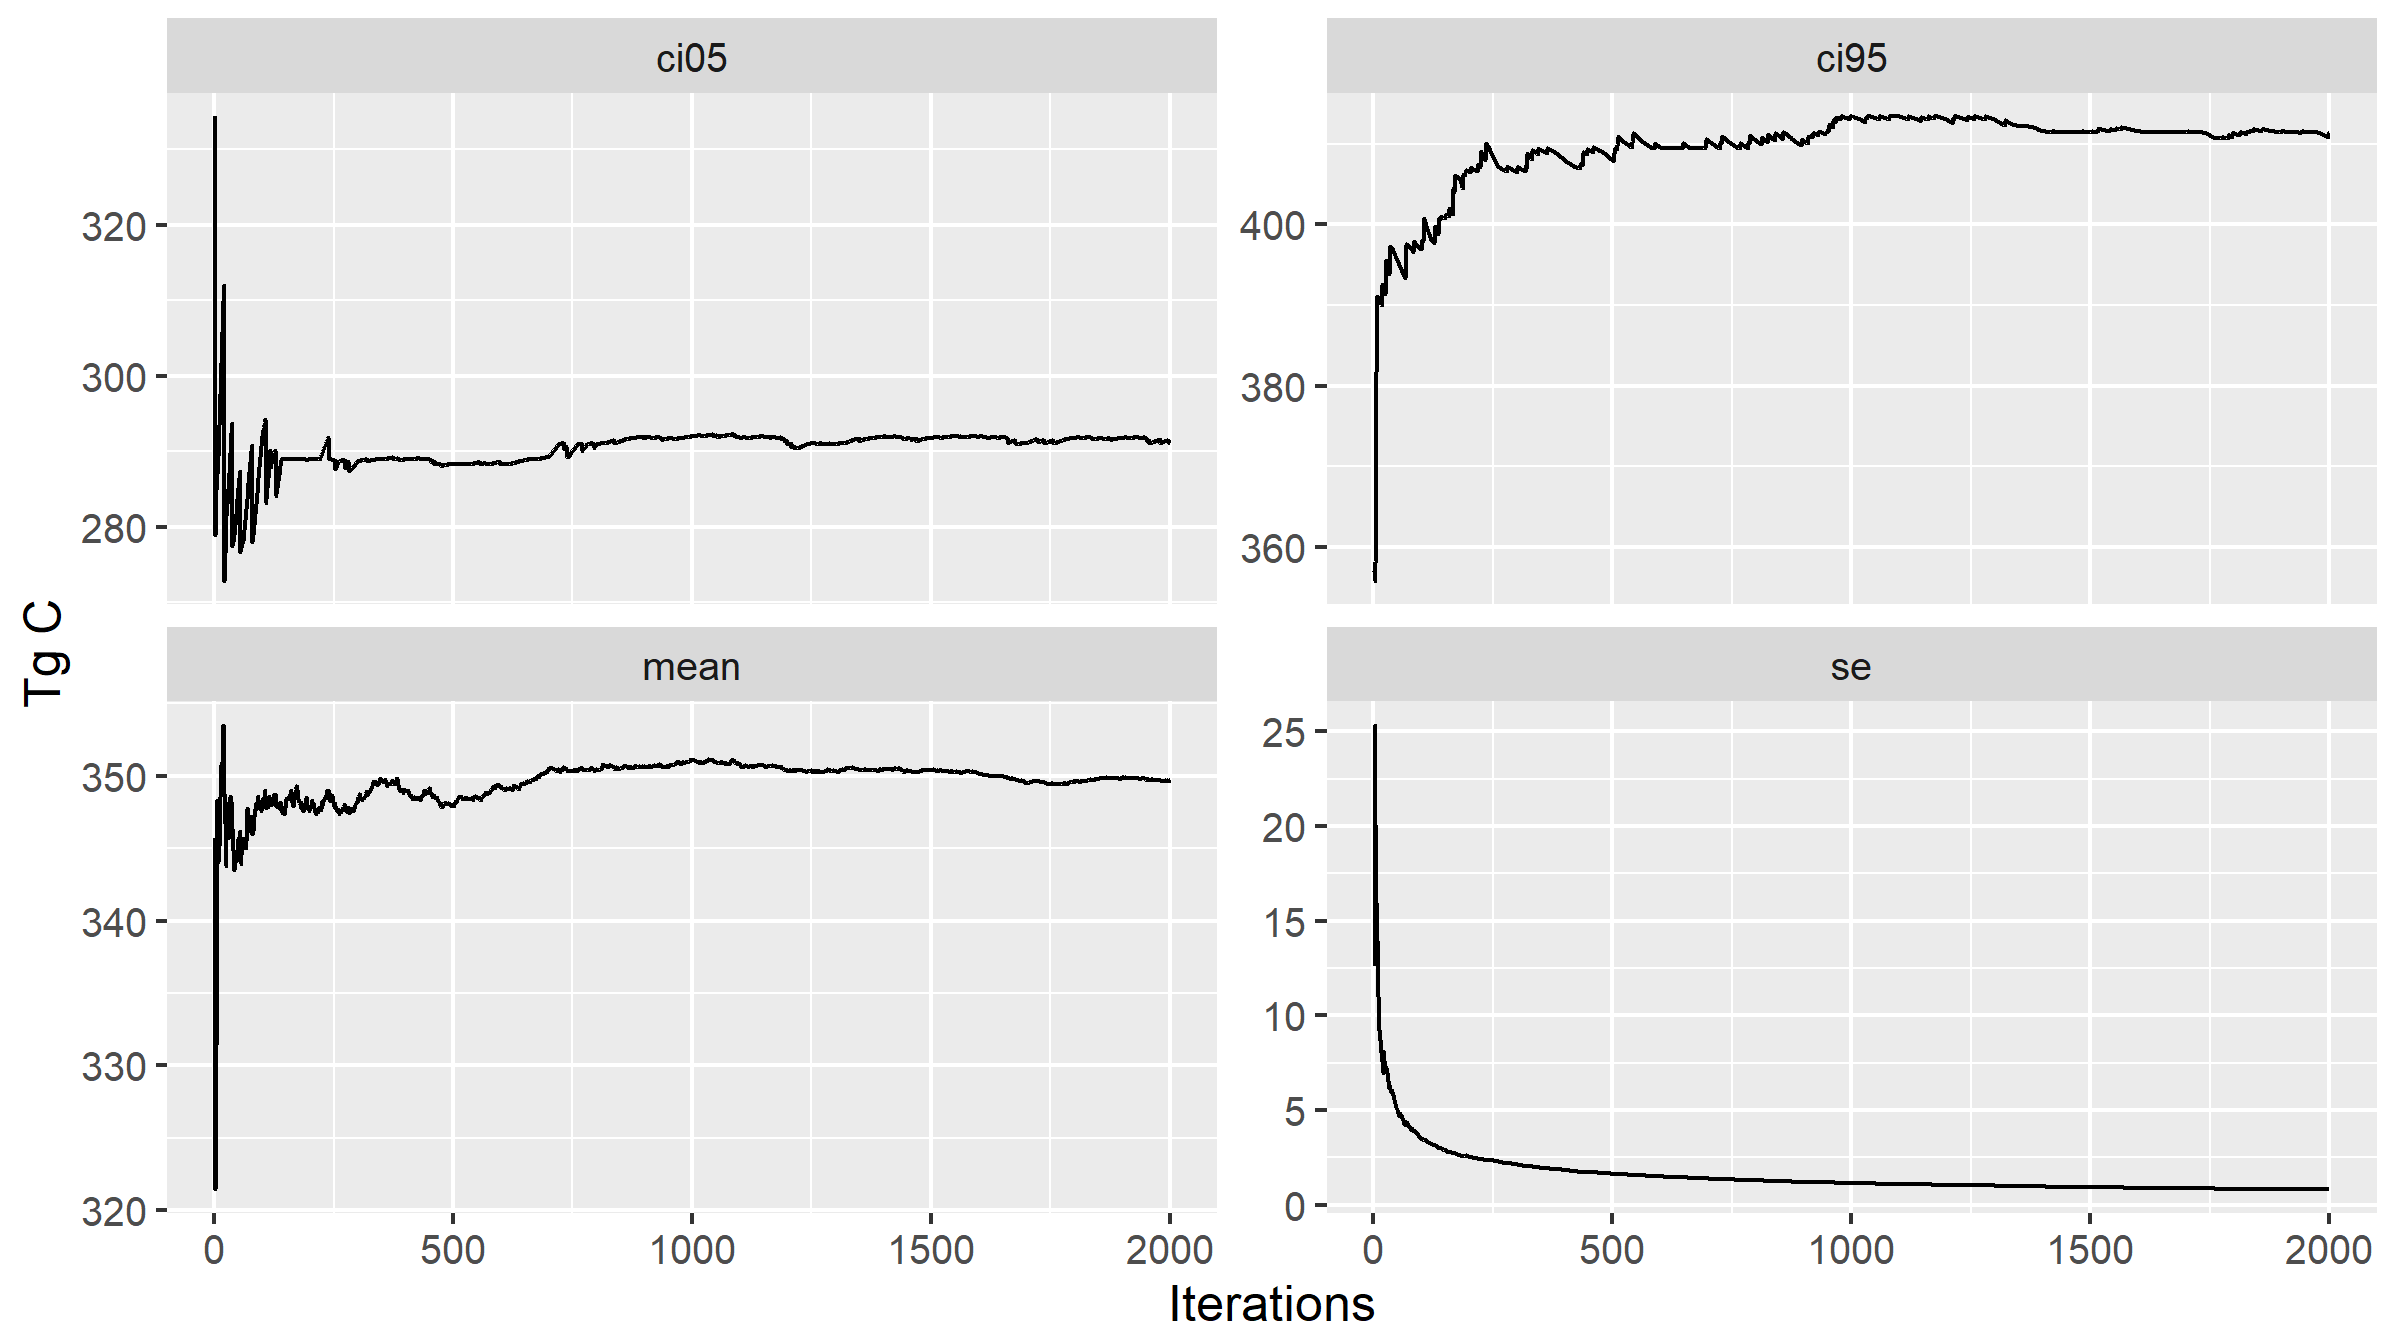
\includegraphics[width=1\linewidth]{images/MC_conv} \caption{Monte Carlo convergence assessment for the upper and lower limits of the empirical 90\% confidence interval, the mean, and the standard error for the full model.}\label{fig:mc-conv-fig}
\end{figure}

The Monte Carlo outputs are summarized in Figures @ref(fig:mc-all4-fig)
and @ref(fig:mc-piu-swds-fig). In Figure @ref(fig:mc-all4-fig) we see
the mean Tg C value for emissions (Emitted with Energy Capture, Emitted
Without Energy Capture) and pools (Products in Use, SWDS) along with the
empirical 90\% confidence intervals. Figure @ref(fig:mc-piu-swds-fig)
combines Products in Use and SWDS into a single carbon pool. The four
carbon fates in Figure @ref(fig:mc-all4-fig) were obtained by
calculating, for each iteration, the cumulative sum of carbon for each
fate across all years. Each fate has 2000 MC iterations for each year.
In Figure @ref(fig:mc-piu-swds-fig), it is difficult to tell, but the
confidence interval range between 1906 and 1920 are between -37\% and +
42\% of the mean. In 2017 the range is between -17\% and +17\% of the
mean.

The correlation procedure described above appeared to work. Table
@ref(tab:ppr-cor-tab) contains the estimated correlation coefficients
for the three triangular distribution random variables used for Primary
Products Ratios. The target correlation coefficient was 0.5.

\begin{table}

\caption{\label{tab:ppr-cor-tab}Correlation matrix for Primary Products Ratios random variables, 2000 draws.}
\centering
\begin{tabular}[t]{cccc}
\toprule
Variables & Variable 1 & Variable 2 & Variable 3\\
\midrule
Variable 1 & 1.000 & 0.505 & 0.508\\
Variable 2 & 0.505 & 1.000 & 0.521\\
Variable 3 & 0.508 & 0.521 & 1.000\\
\bottomrule
\end{tabular}
\end{table}

\begin{figure}
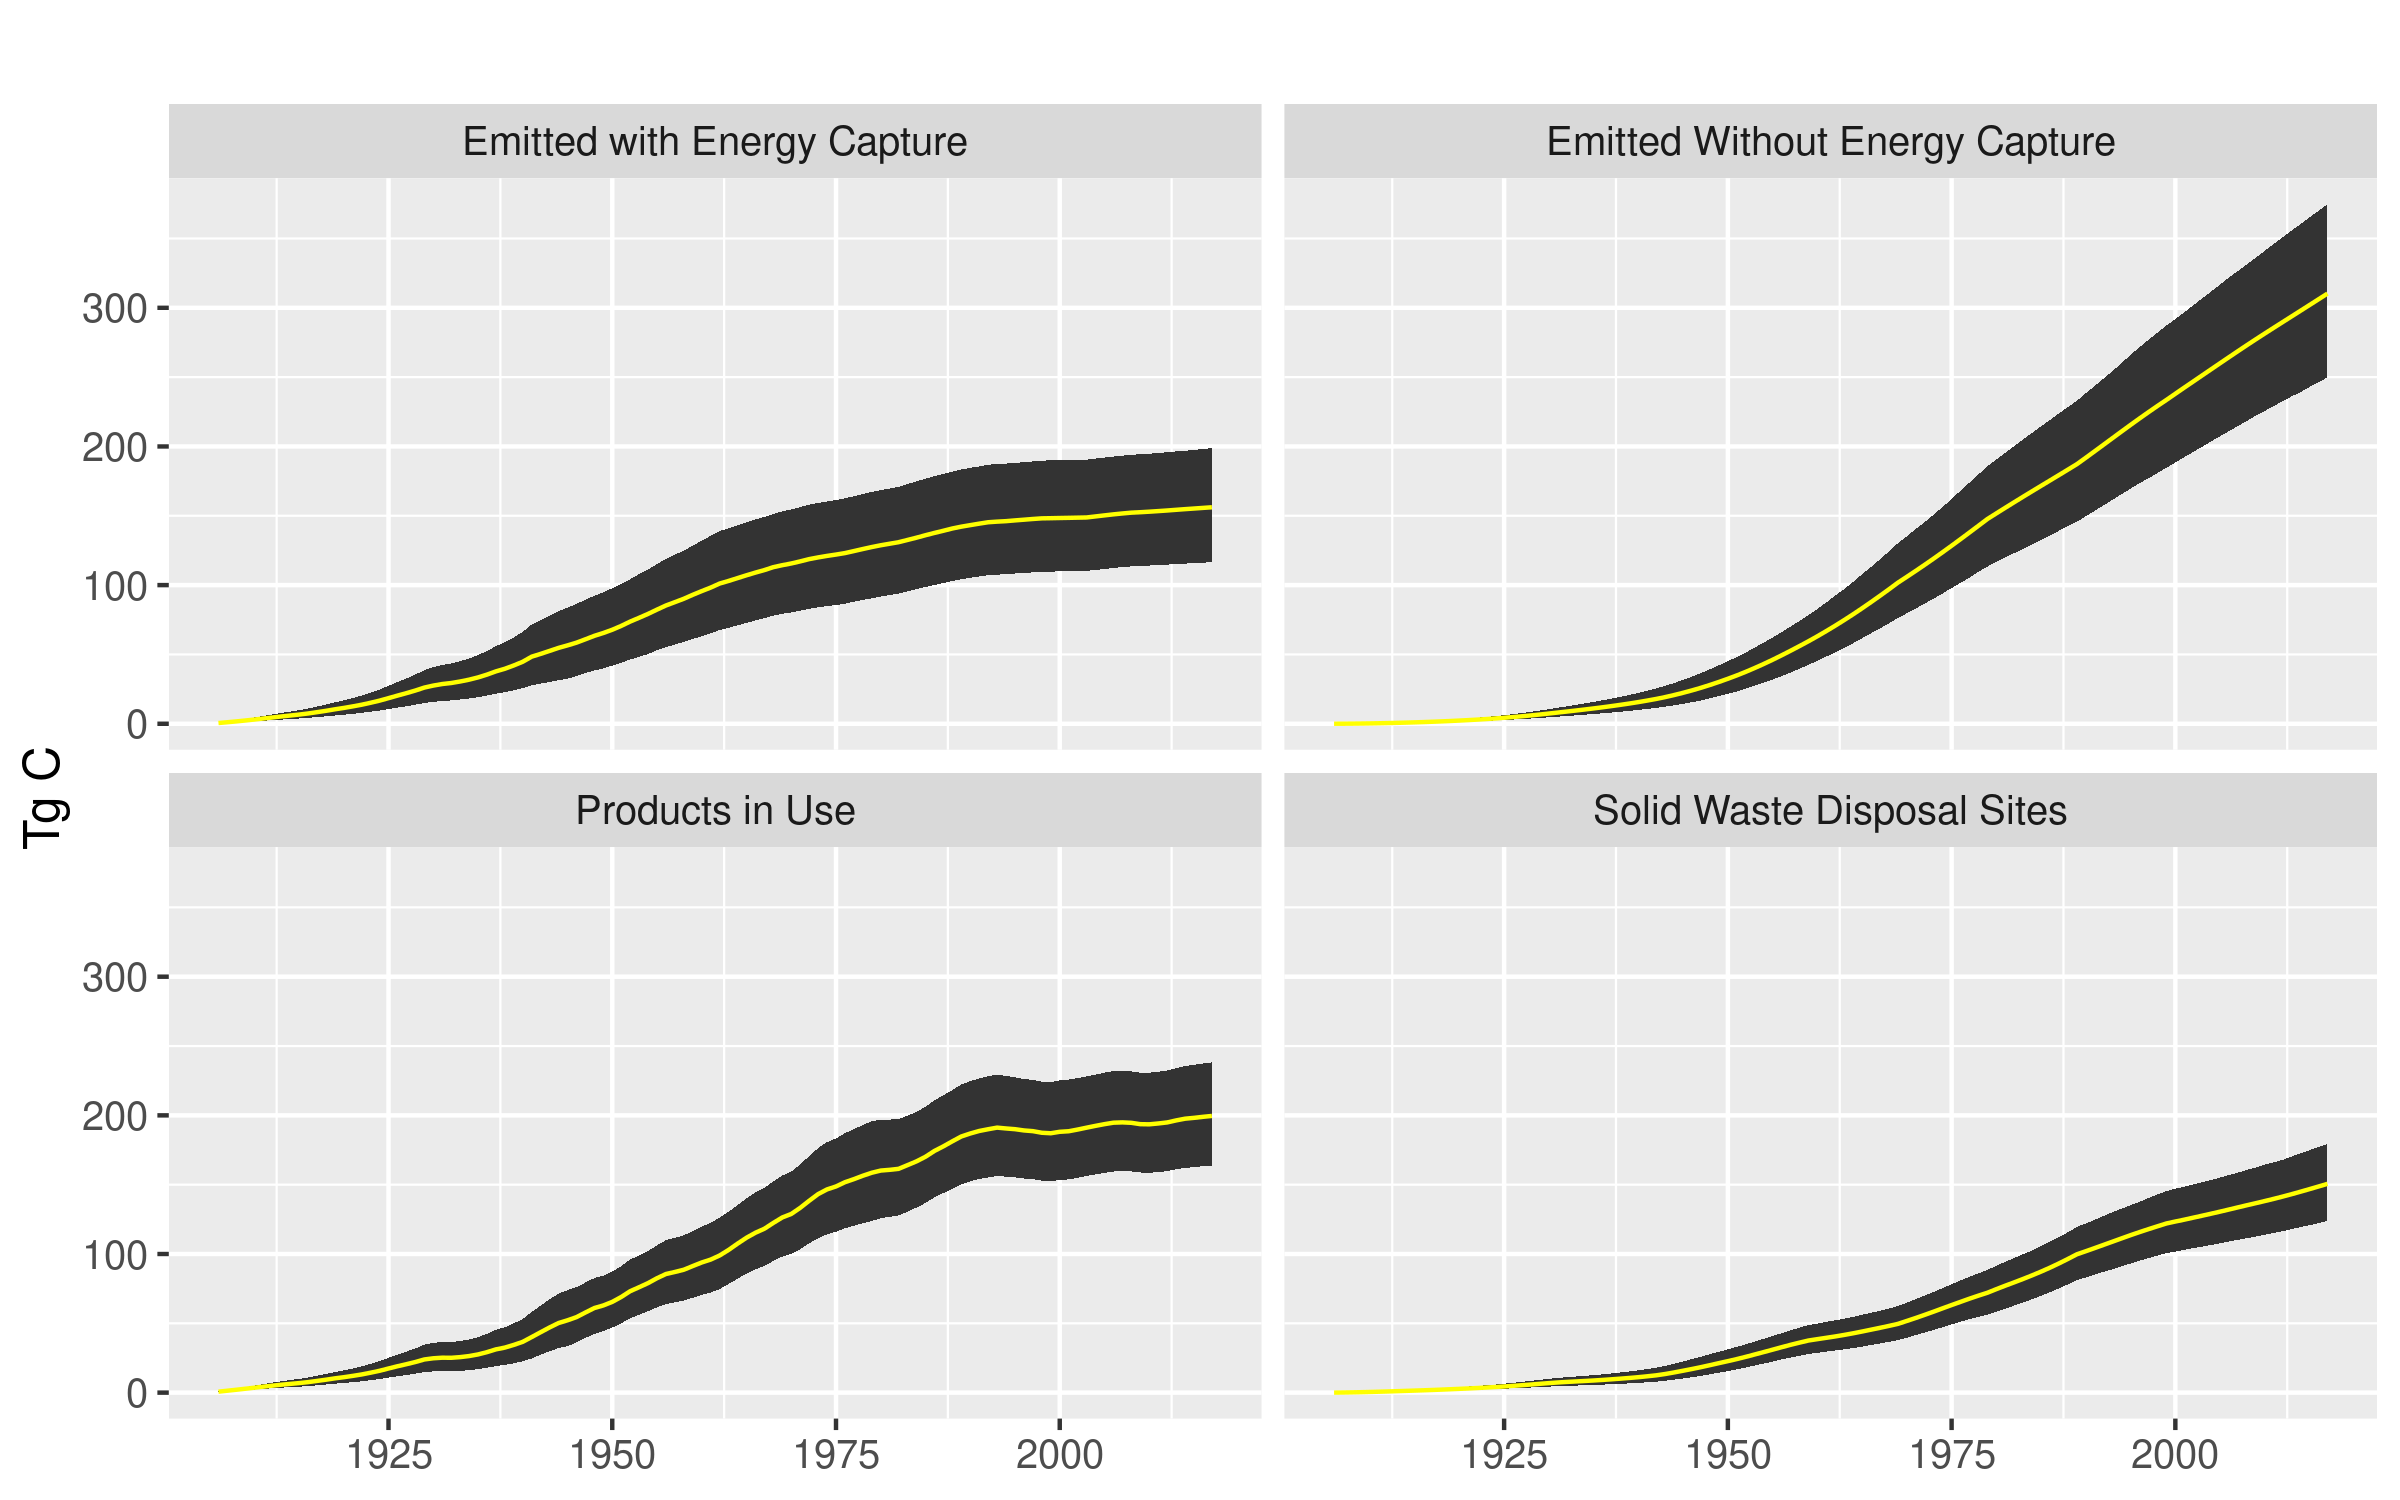
\includegraphics[width=1\linewidth]{images/MC_all4} \caption{Monte Carlo simulation mean (yellow) and 90\% confidence interval ranges for four HWP carbon fates across years.}\label{fig:mc-all4-fig}
\end{figure}

\begin{figure}
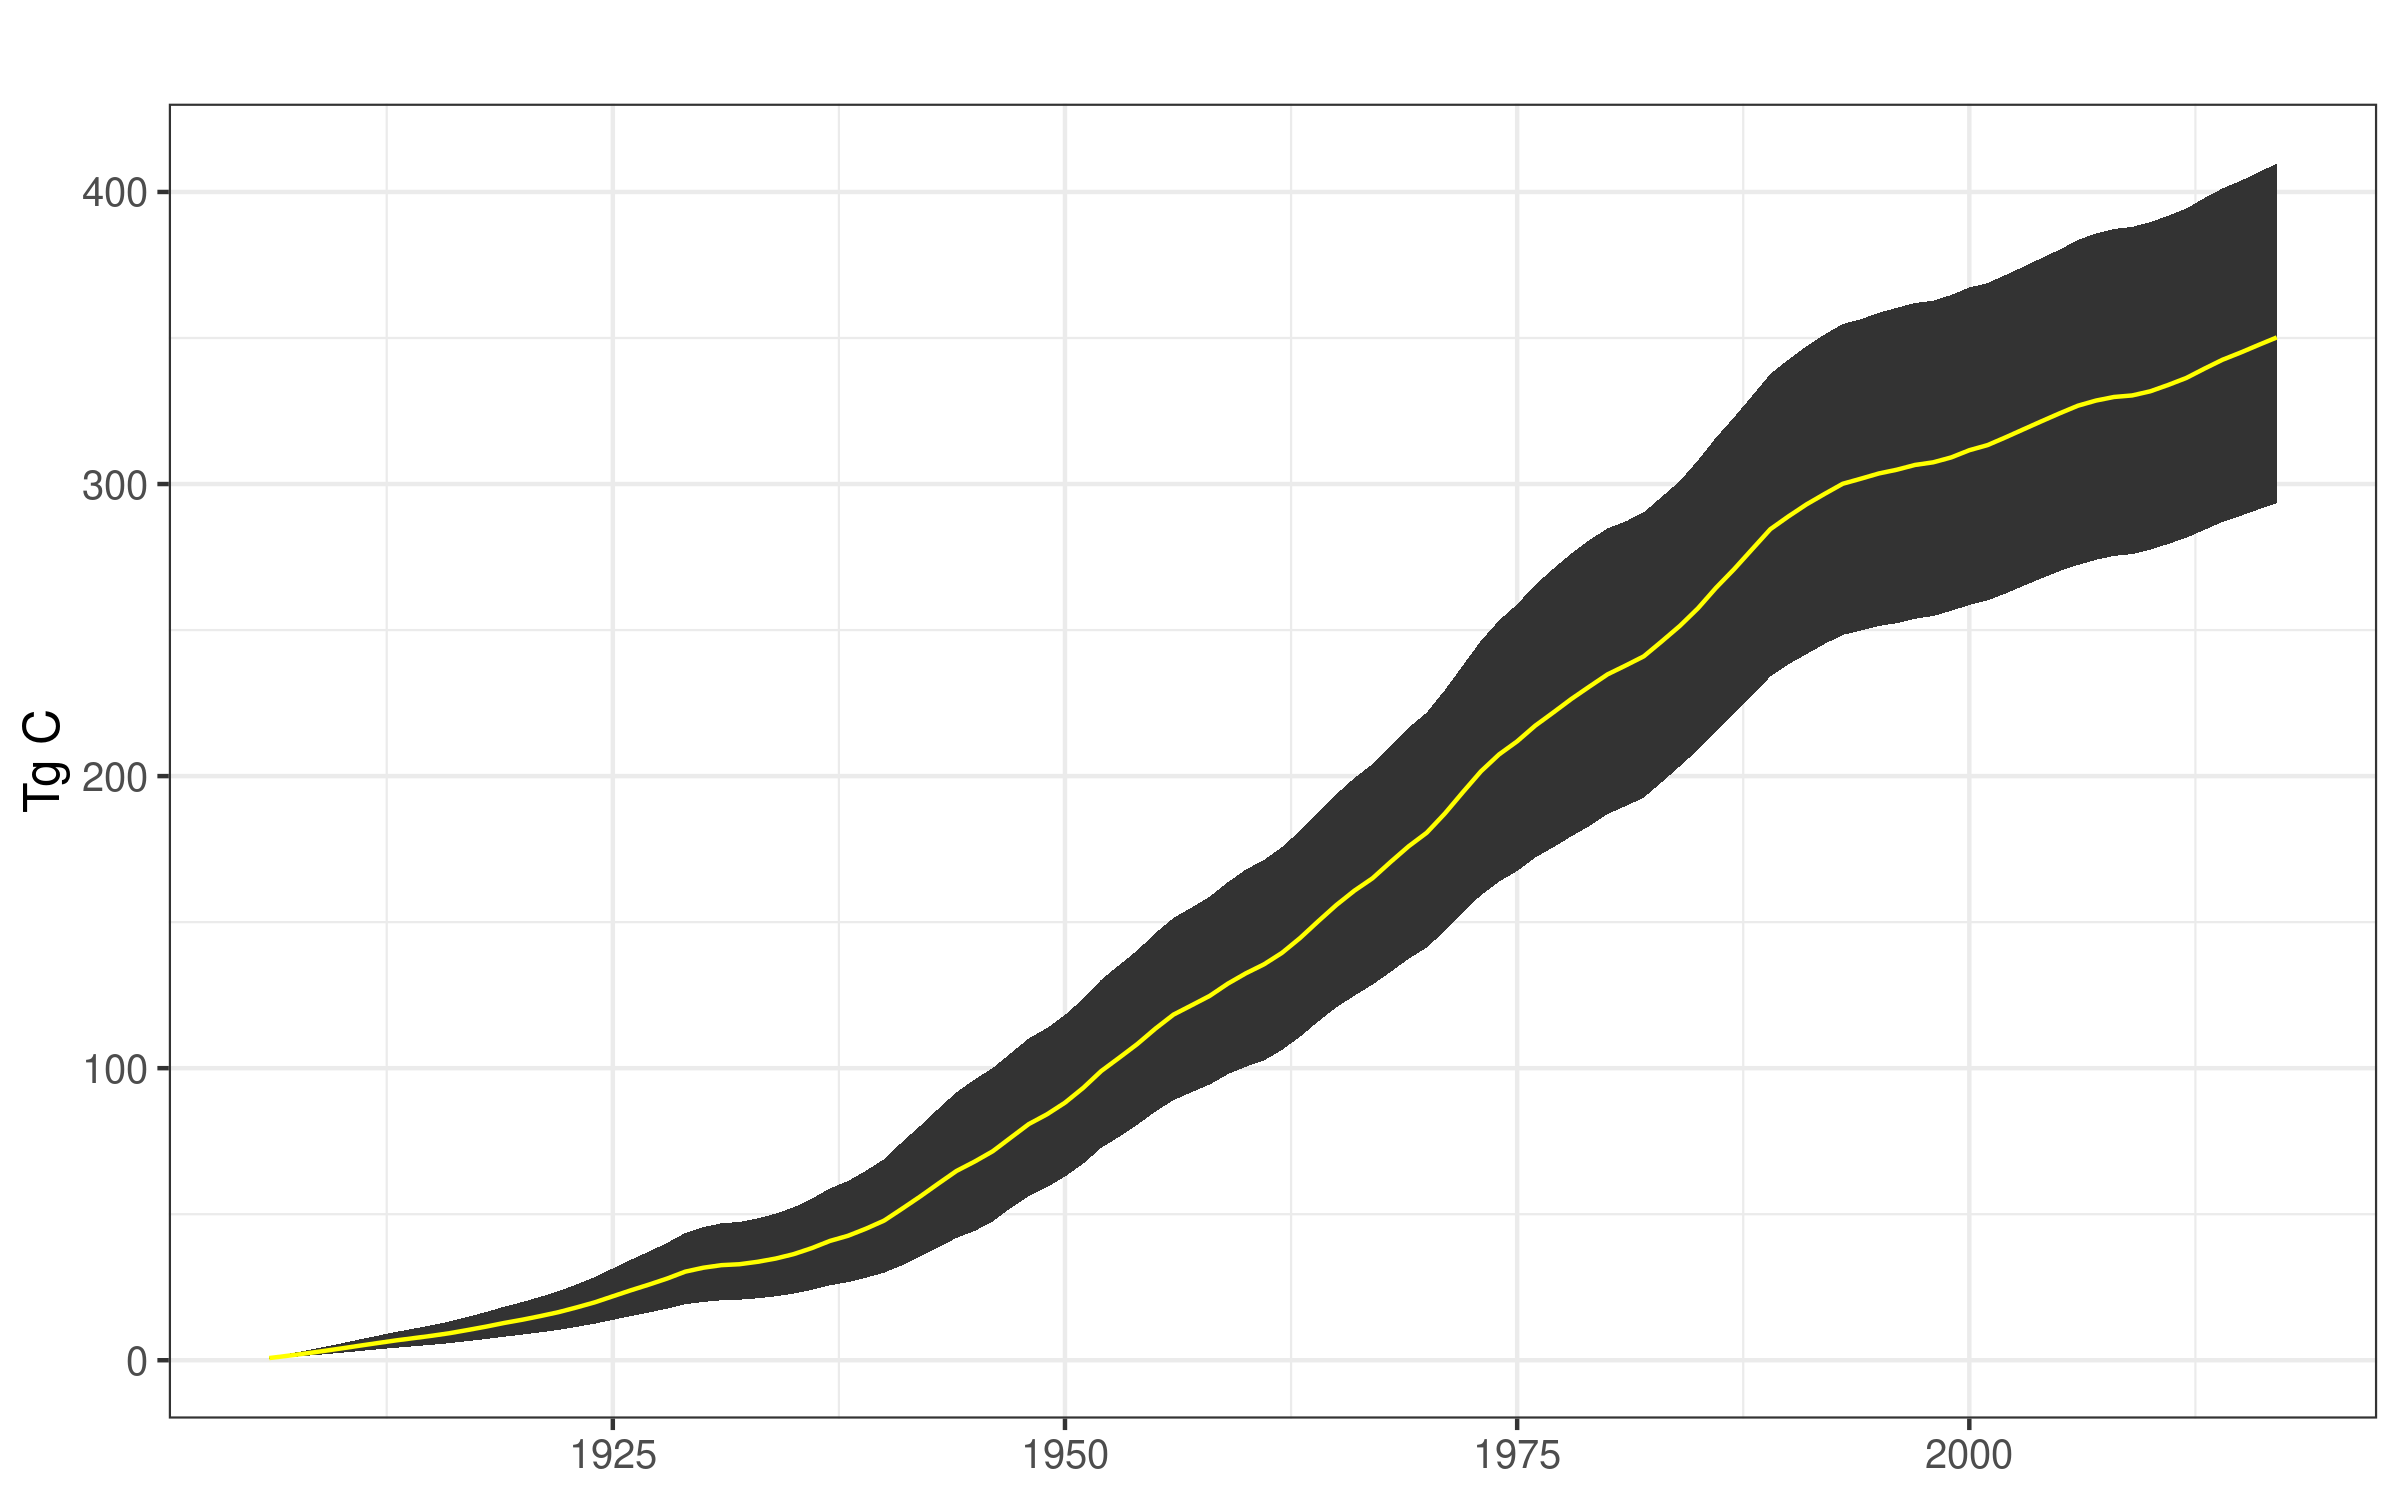
\includegraphics[width=1\linewidth]{images/MC_piu_swds} \caption{Monte Carlo simulation mean (yellow) and 90\% confidence interval ranges for the total Tg C value for SWDS and Products in Use.}\label{fig:mc-piu-swds-fig}
\end{figure}

Histograms of the three vectors of Primary Products Ratios triangular
random variables are presented in Figure @ref(fig:mc-tri1-fig). The
values are correlated (Table @ref(tab:ppr-cor-tab)) and the histogram
distributions correspond to 90\% confidence intervals and endpoints (see
Table @ref(tab:triang-tab) for triangular distribution endpoints for
0.7-1.3, 0.8-1.2, and 0.85-1.15 90\% confidence intervals). Although
Variables 2 and 3 do not evidence as tight a triangular distribution as
Variable 1, their distributions appear approximately triangular and do
not appear skewed.

Figures @ref(fig:mc-tri2-fig) and @ref(fig:mc-tri3-fig) examine
triangular distribution changes on sum-to-one ratio sets. In Figure
@ref(fig:mc-tri2-fig), PPR.21 is the largest proportion in its
sum-to-one group of proportions and was directly adjusted by the random
triangular variable draws. PPR.17 was adjusted to ensure that it and the
other variables in the group still summed to one. Note that although
PPR.21 was the only one directly altered, PPR.17 evidences a triangular
distribution as well. The percentage range of PPR.17 values was broader,
however, than the percentage range of values for PPR.21.

Figure @ref(fig:mc-tri3-fig) shows the consequences of altering a
sum-to-one ratio beyond 1.0, in this case using TPR.2 during the year
2002. The code truncates the value at 1.0, forcing TPR.1 to become zero.
The two ratio sets appear to otherwise conform to triangular
distributions.

\begin{figure}
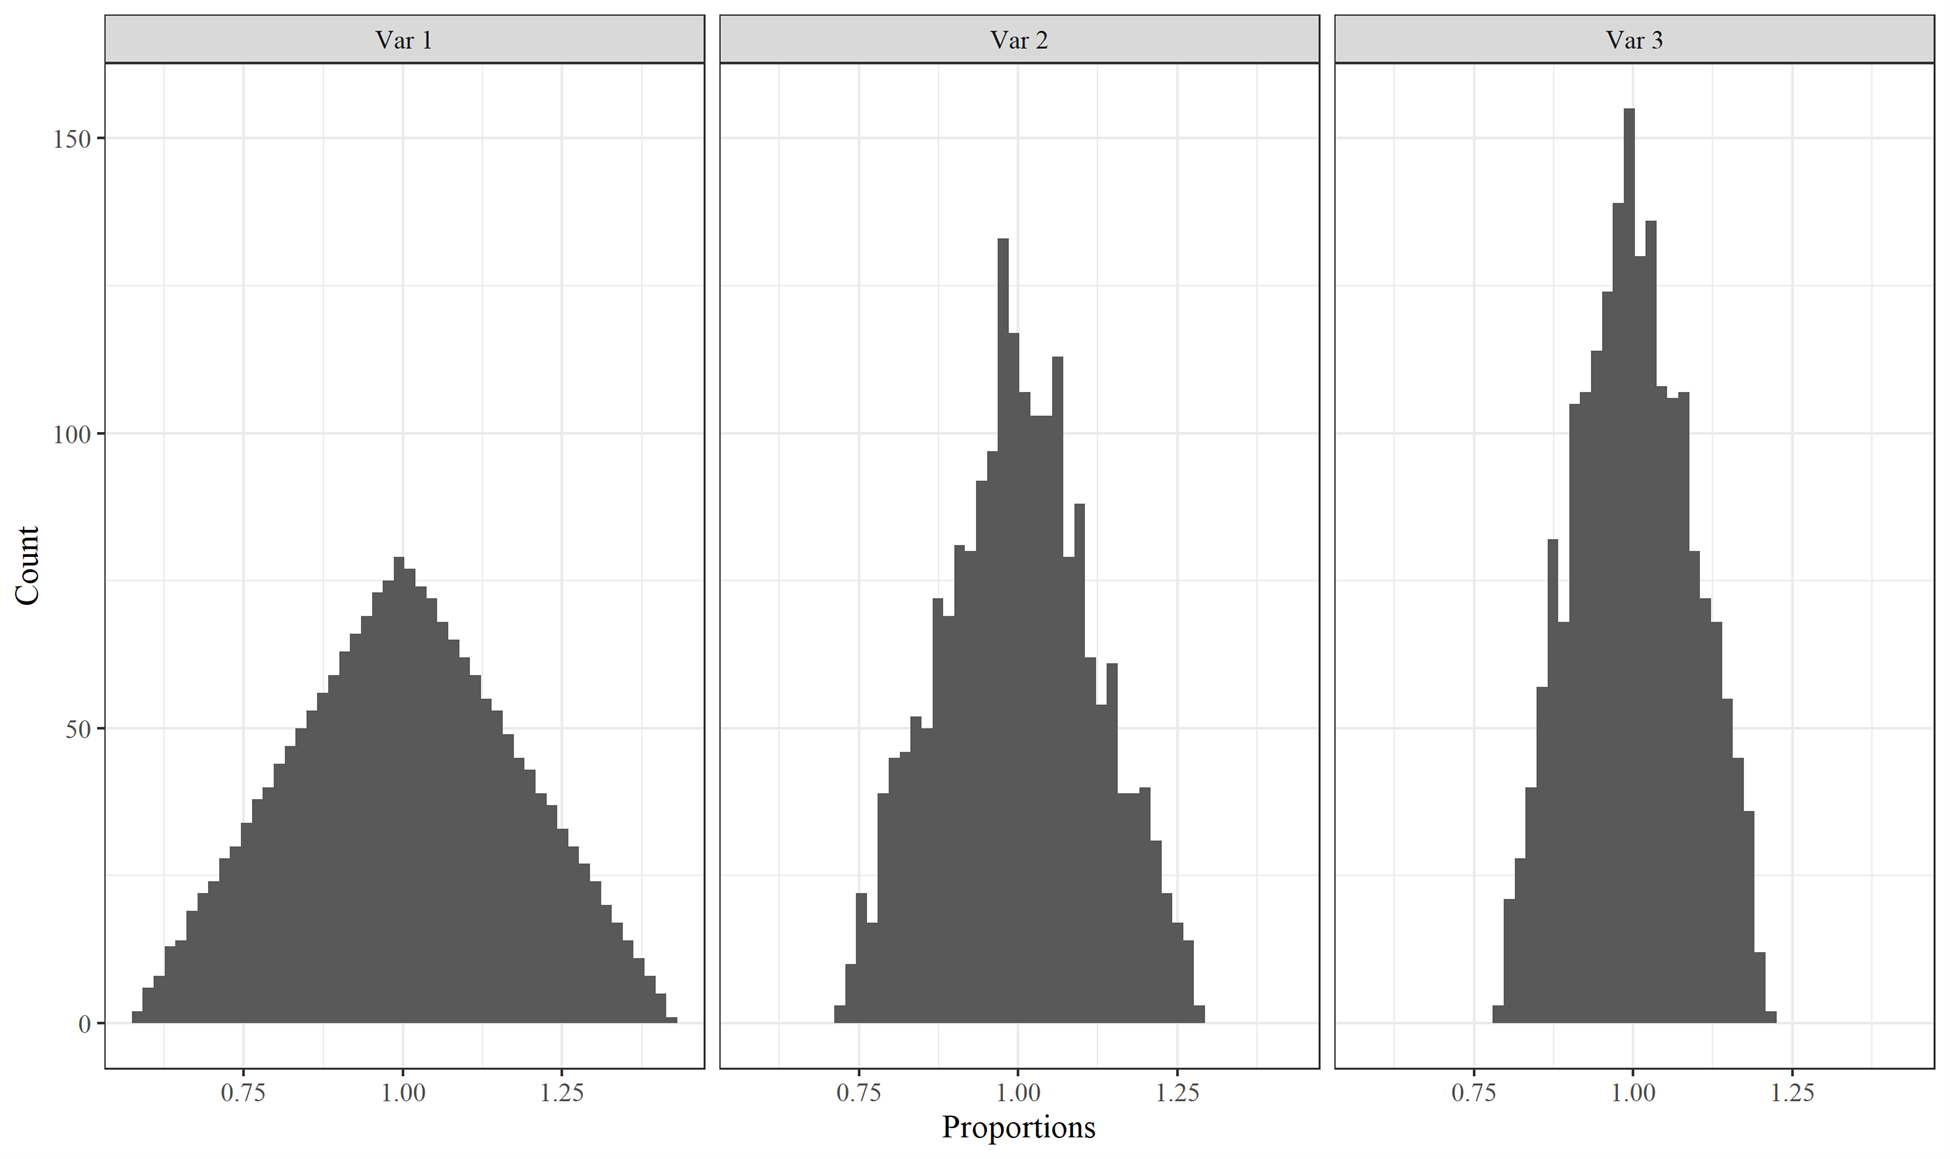
\includegraphics[width=1\linewidth]{images/triang1} \caption{Histograms of correlated triangular distribution random variables for Primary Product Ratios.}\label{fig:mc-tri1-fig}
\end{figure}

\begin{figure}
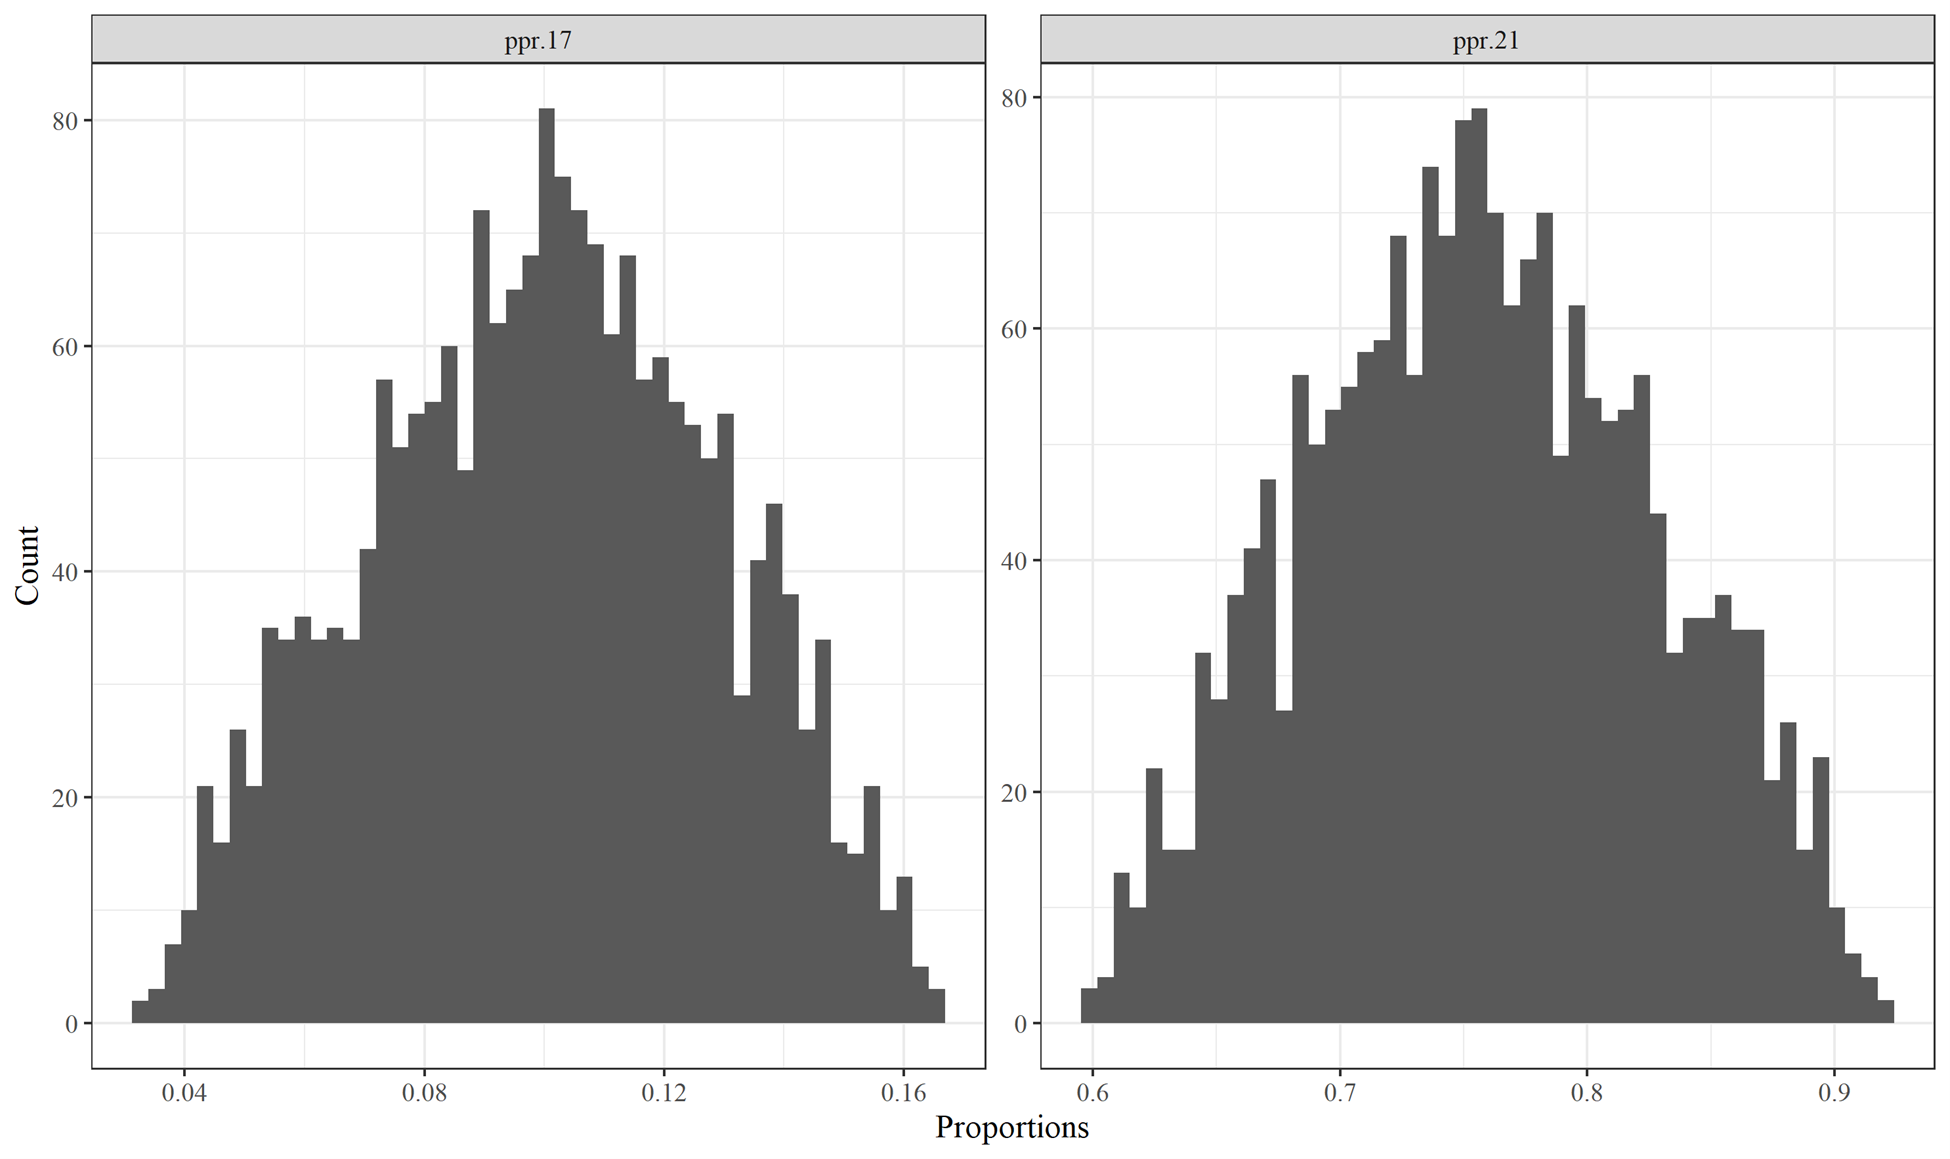
\includegraphics[width=1\linewidth]{images/triang2} \caption{Histograms of sum-to-one Primary Product Ratios variables PPR.17 and PPR.21 that do not overlap with 0.0 or 1.0.  Both variables are for the year 1994.}\label{fig:mc-tri2-fig}
\end{figure}

\begin{figure}
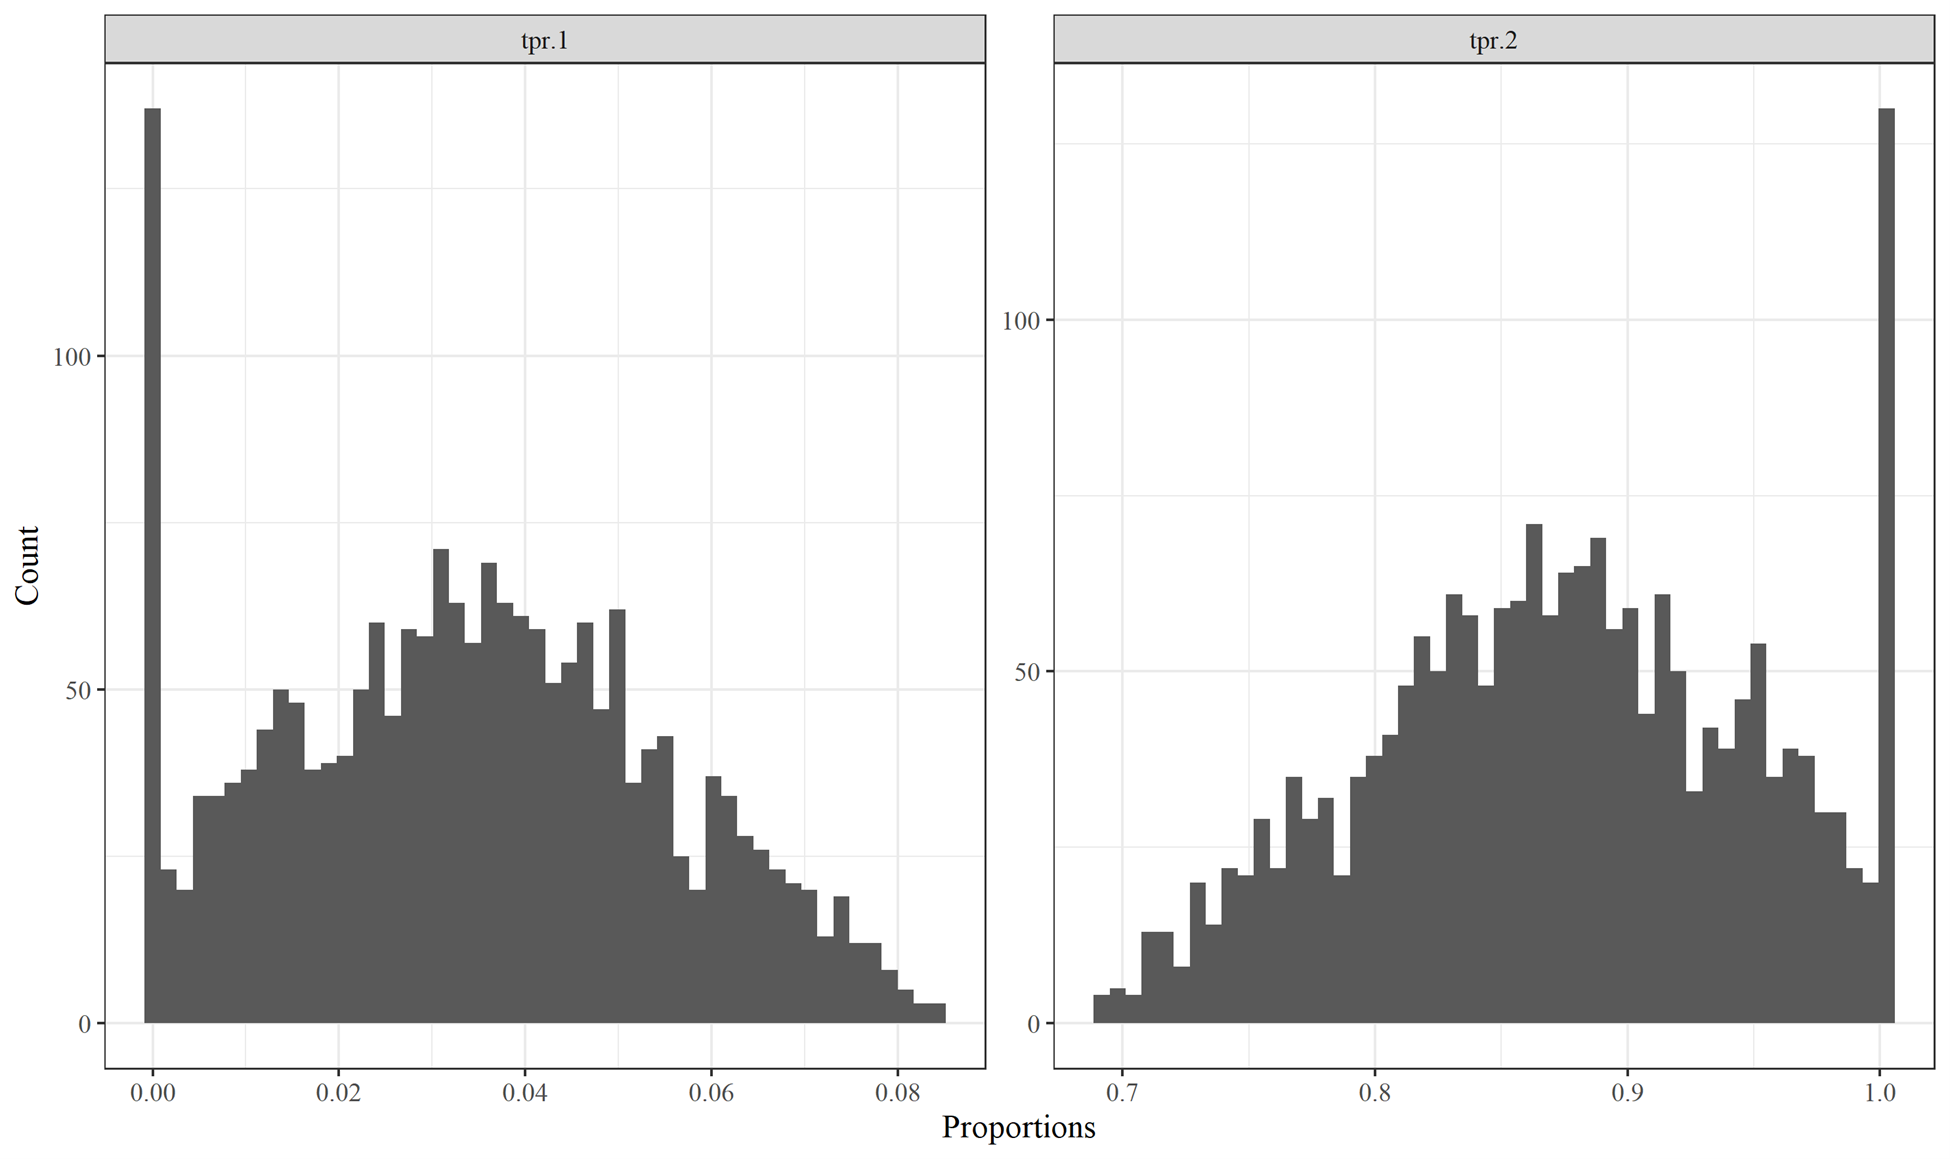
\includegraphics[width=1\linewidth]{images/triang3} \caption{Histograms of sum-to-one Timber Product Ratios variables TPR.1 and TPR2; the values for TPR.2 were truncated at 1.0.  Both variables are for the year 2002.}\label{fig:mc-tri3-fig}
\end{figure}

The MC simulation was developed in pieces. We first altered the values
for the non-sum-to-one variables: CCF to MgC conversion factors, annual
harvest amounts, product half-lives, landfill decay limits, and the
half-lives of decaying paper and wood in landfill, dumps, and recovered
products. These alterations should affect all categories, since harvest
amounts and the conversion factors control all carbon input into the
model, product half-lives affect PIU residence and SWDS input, and the
SWDS decay limits and half lives affect residency in SWDS.

We next introduced Timber Production Ratios as the first sum-to-one MC
alterations, then Primary Production Ratios, then End Use Ratios.
Finally, we added the Discarded Disposition Ratios (DDR). These
additions did not affect MC results for all carbon fates (Emitted with
Energy Capture, Emitted without Energy Capture, Solid Waste Disposal
Sites, and Products in Use) equally.

Figure @ref(fig:mc-tests-fig) provides results for Emitted with Energy
Capture. We can see that the MC 90\% confidence intervals increase
between the first (No Sum-to-One MC Variables) and second (TPR) versions
of the model. When we introduced variation into the Timber Production
Ratios and then Primary Product Ratios the ratios for fuel wood were
altered. Those fuel wood ratios are not altered by changes to EUR, as
EUR in this case effectively serves as a ``pass-through'' category for
fuel wood where the ratios remain 1.0 and are not altered by the
simulation.

\begin{figure}
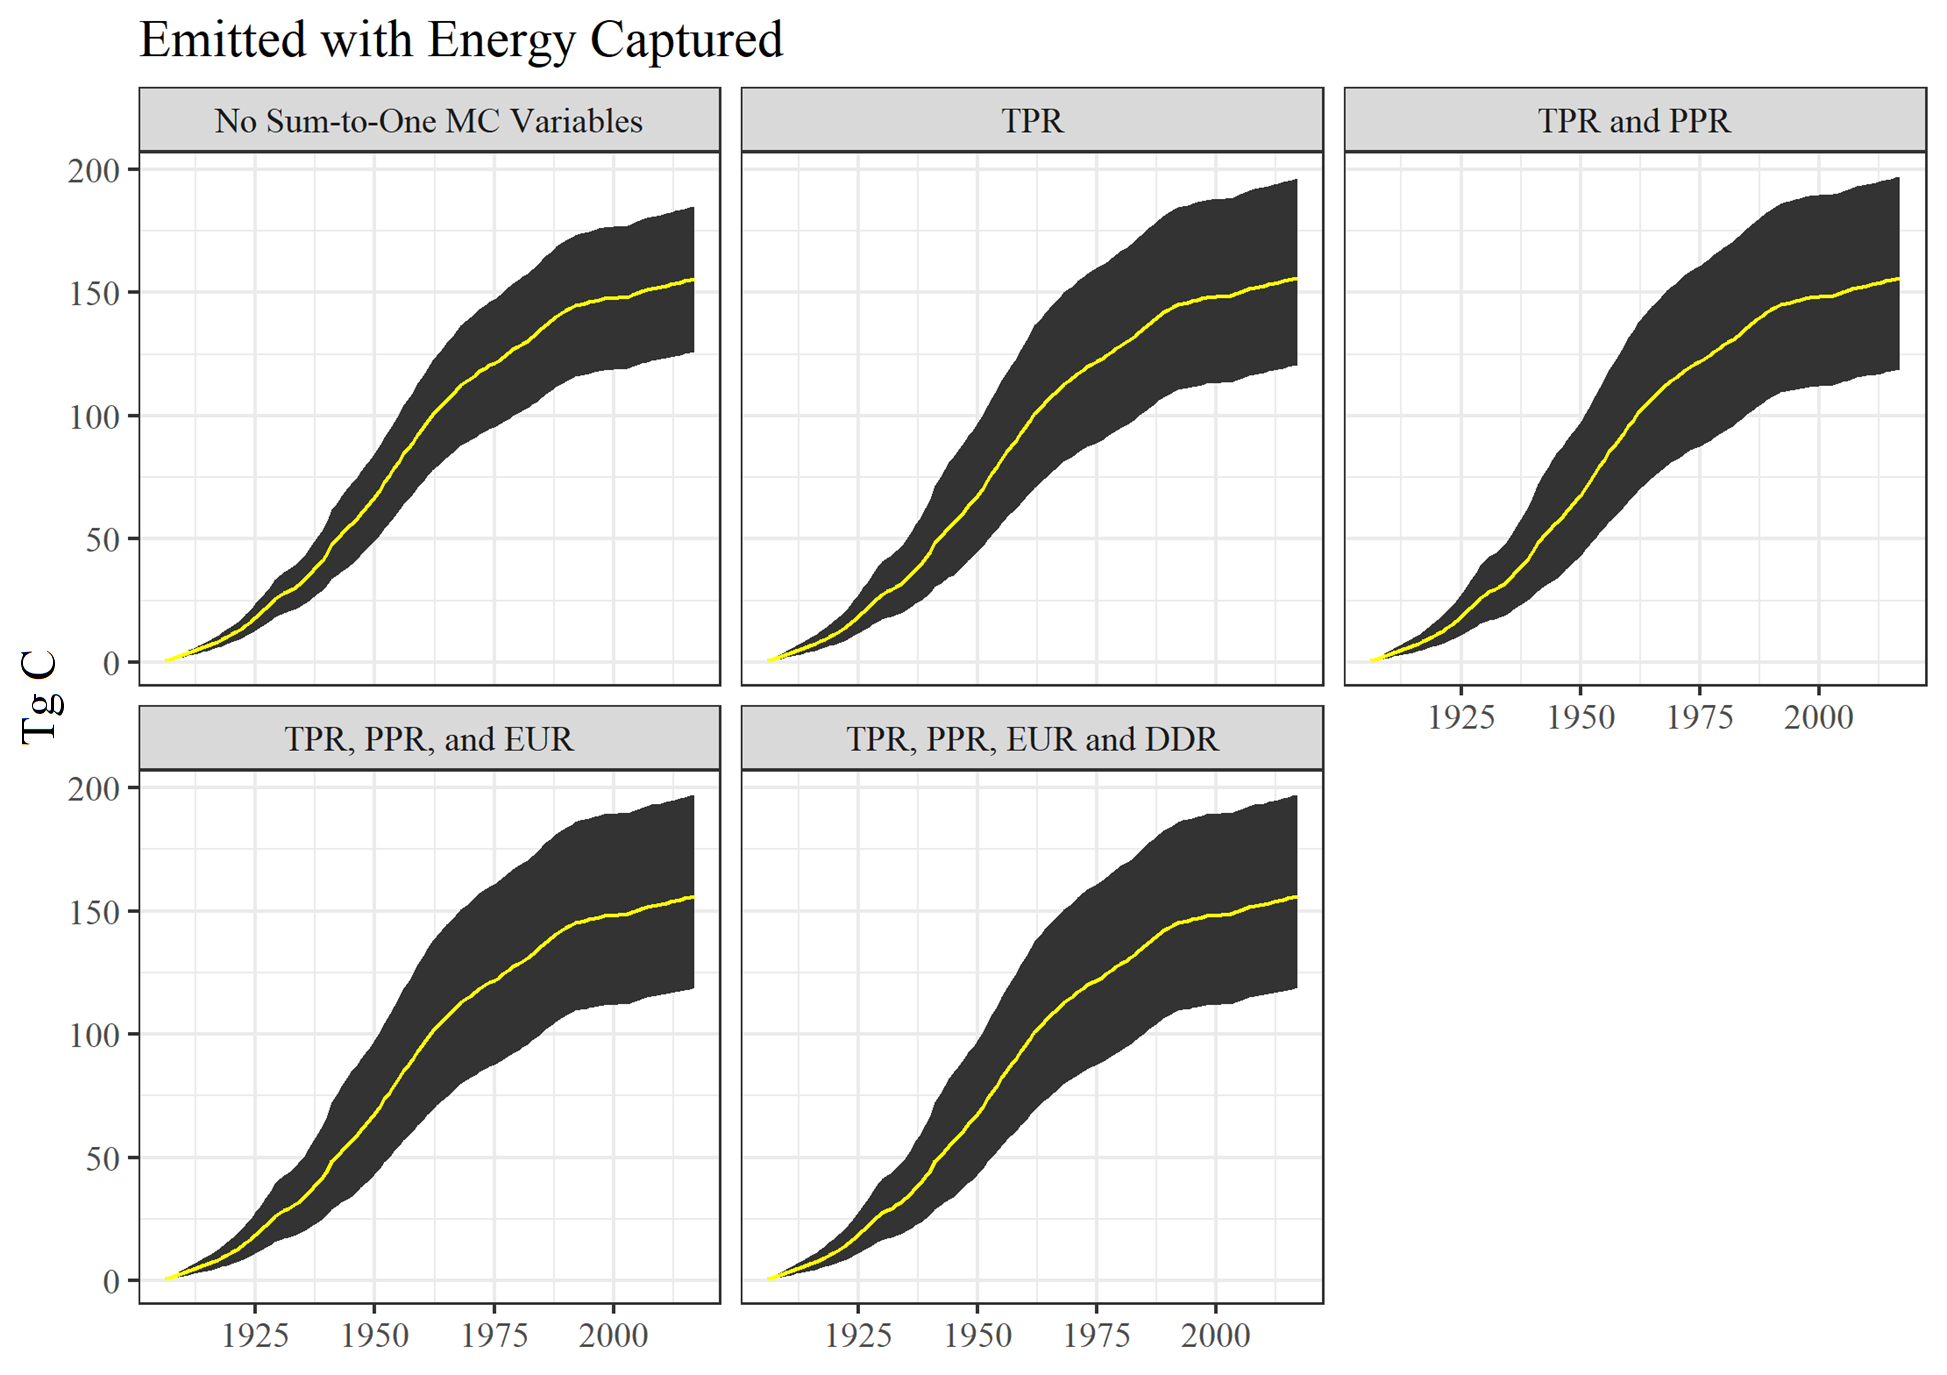
\includegraphics[width=1\linewidth]{images/MC_tests} \caption{Monte Carlo simulation outputs for Emitted with Energy Captured for different Monte Carlo construction stages.  See text for acronym definitions.}\label{fig:mc-tests-fig}
\end{figure}

Figure @ref(fig:mc-tests2-fig), Emitted without Energy Capture, is
interesting because graphically there does not appear to be a large
change between MC construction iterations. However, the confidence
interval ranges do increase across all versions. Each version differs by
between 1 and 4\% of the previous version. Therefore, most of the gain
in variability was achieved by altering the first set of variables. All
other variable alterations did affect the amount of carbon emitted
without energy capture, be it affecting the discard dispositions or the
End Use Product Ratios (which would in turn be affected by EUR product
half-lives and all other variables affecting the next steps of disposal
and decay). The effect was not large, however.

Figure @ref(fig:mc-tests3-fig), depicting the MC results for carbon
stored in Solid Waste Disposal Sites, really does not evidence an
increase in the MC confidence interval until the final iteration when
Discarded Disposition Ratios are changed. Changing the DDR affects where
disposed carbon winds up. The initial version of the model is already
altering carbon entering the system and product half-lives. These are
likely the two major drivers of variation for SWDS. Altering the ratios
of which products carbon goes to affects things relatively slightly.

\begin{figure}
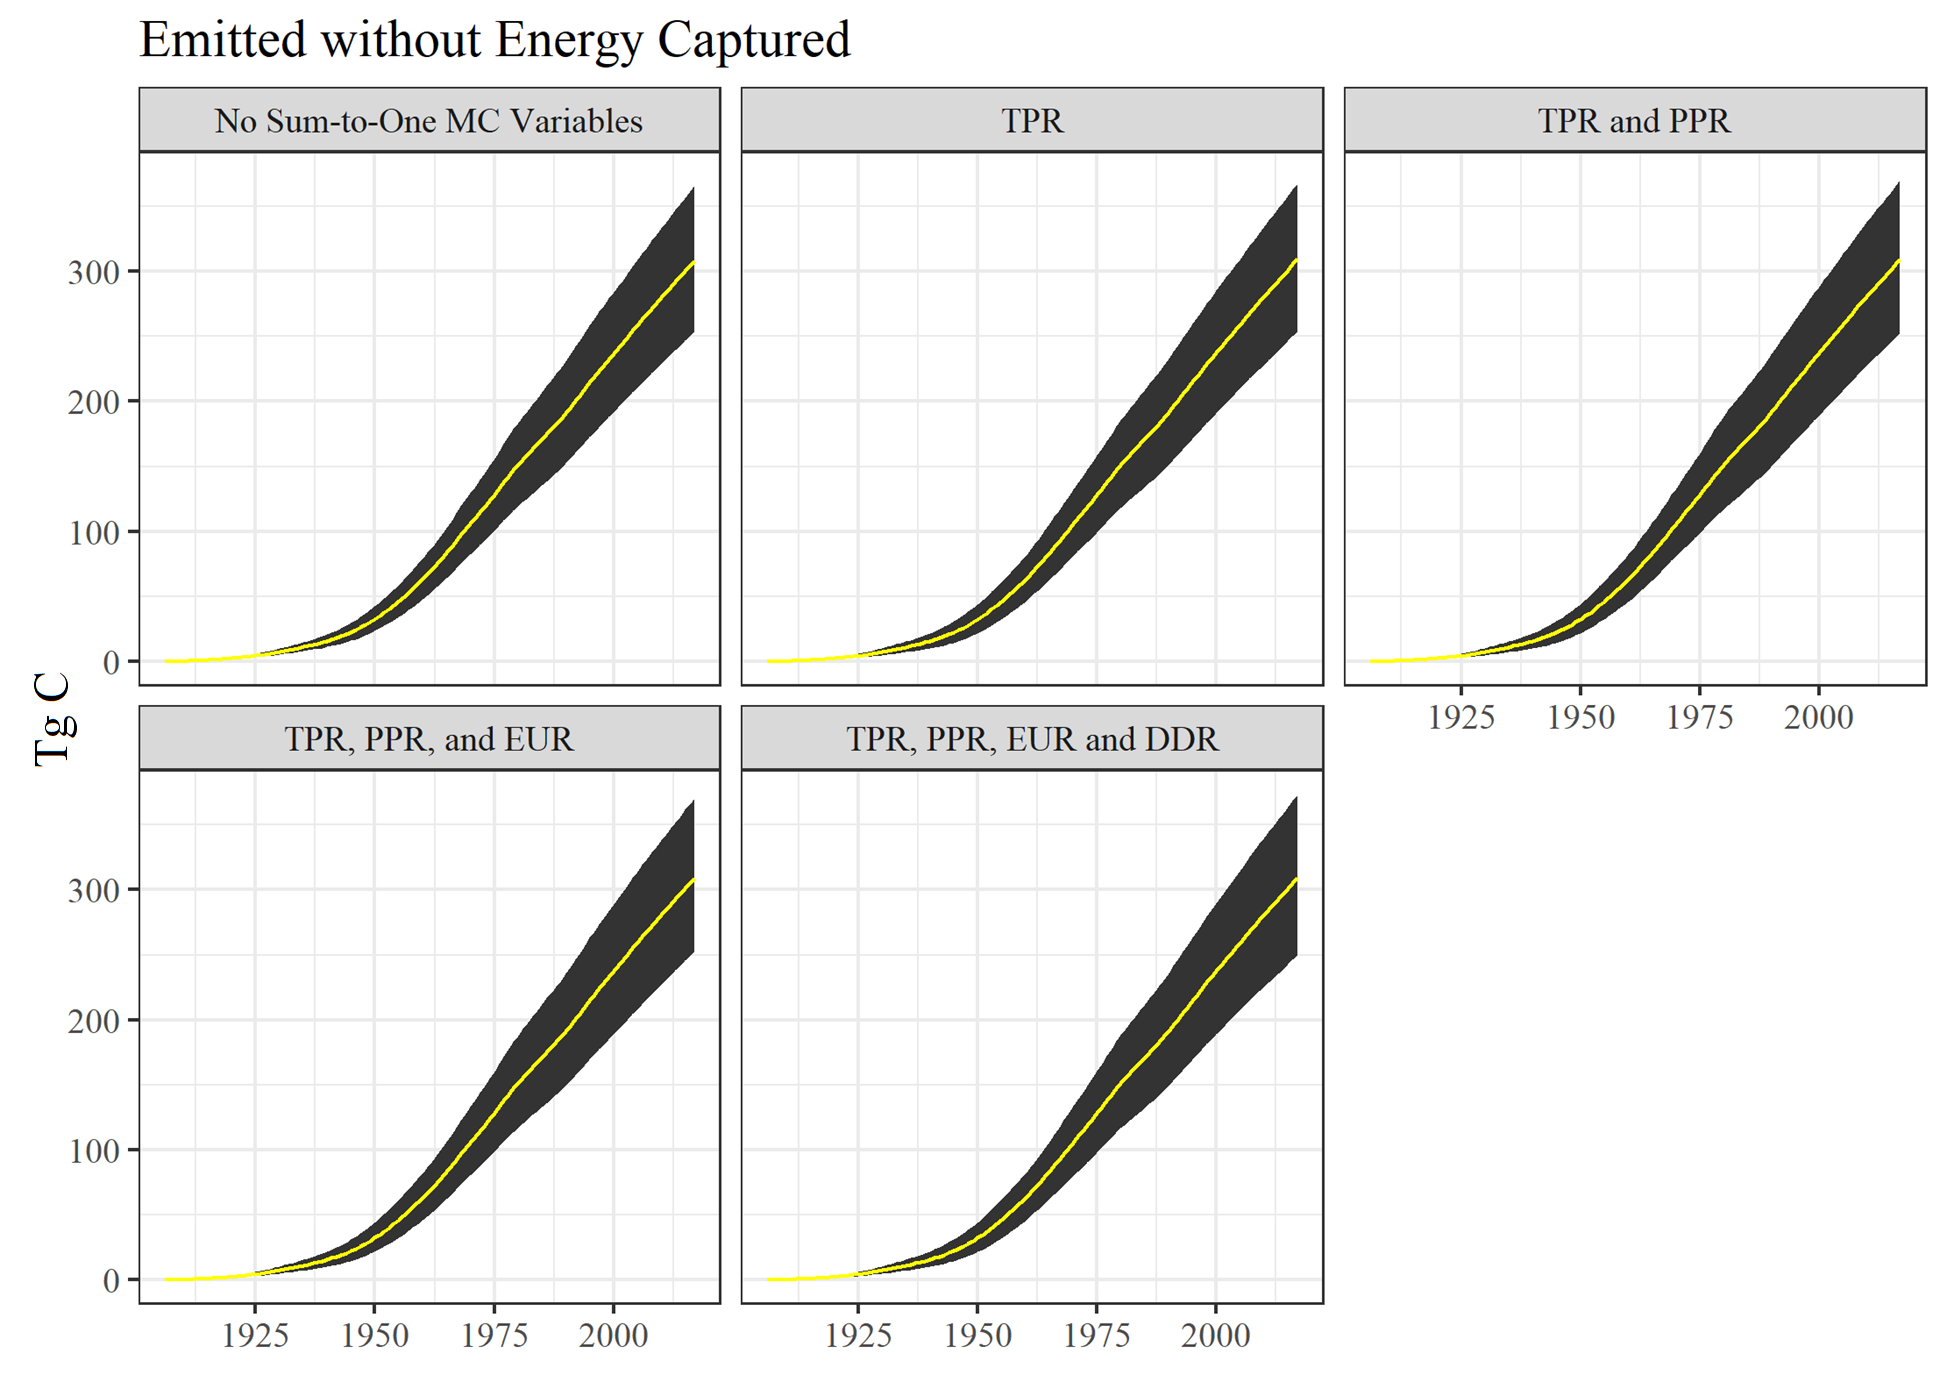
\includegraphics[width=1\linewidth]{images/MC_tests2} \caption{Monte Carlo simulation outputs for Emitted without Energy Captured for different Monte Carlo construction stages.  See text for acronym definitions.}\label{fig:mc-tests2-fig}
\end{figure}

Products in Use (Figure @ref(fig:mc-tests4-fig)) outcomes for the
different MC model versions has similar results as EWOEC. Subsequent
additions of sum-to-one variables do increase the confidence intervals,
by about 1 to 2\%. Therefore, adding the sum-to-one variables did not
affect the model much. As we might expect, including the DDR variable
changes did not affect PIU confidence intervals at all since those
changes only interact with discarded carbon.

\begin{figure}
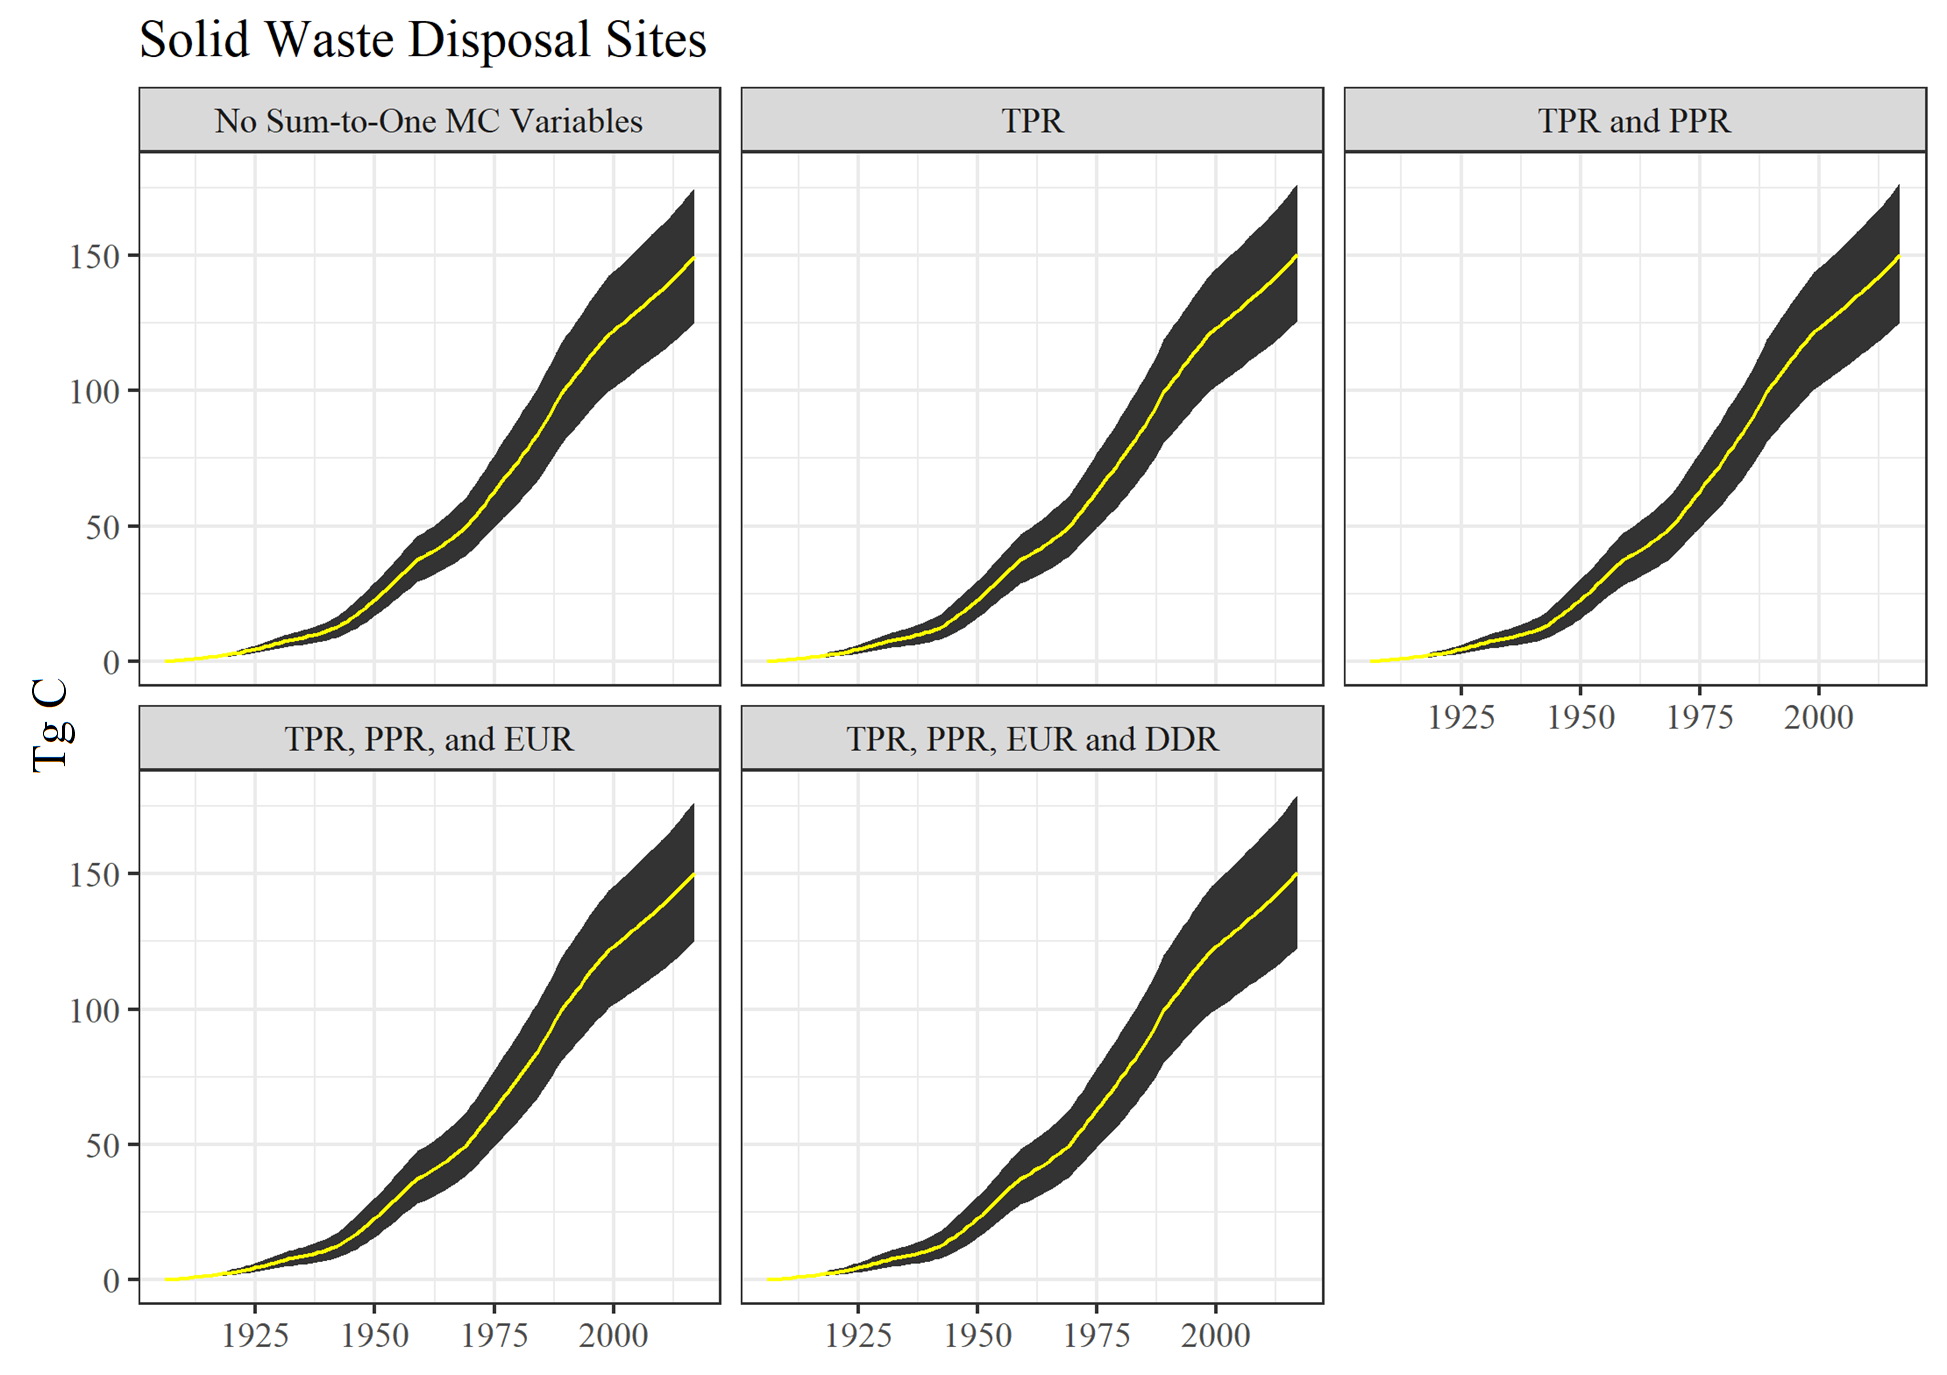
\includegraphics[width=1\linewidth]{images/MC_tests3} \caption{Monte Carlo simulation outputs for Solid Waste Disposal Sites for different Monte Carlo construction stages.  See text for acronym definitions.}\label{fig:mc-tests3-fig}
\end{figure}

The simulation also did not use different random triangular variable
values within a parameter for a given iteration. For instance, the
California and Oregon have 224 product decay ratios. In a single
iteration they were all multiplied by the same draw value from a
triangular distribution. Conceivably, there could be a separate random
draw for every product decay ratio, and every other sort of parameter
subset. This could result in creating a LHS procedure with hundreds of
separate random variables instead of the number used here.

\begin{figure}
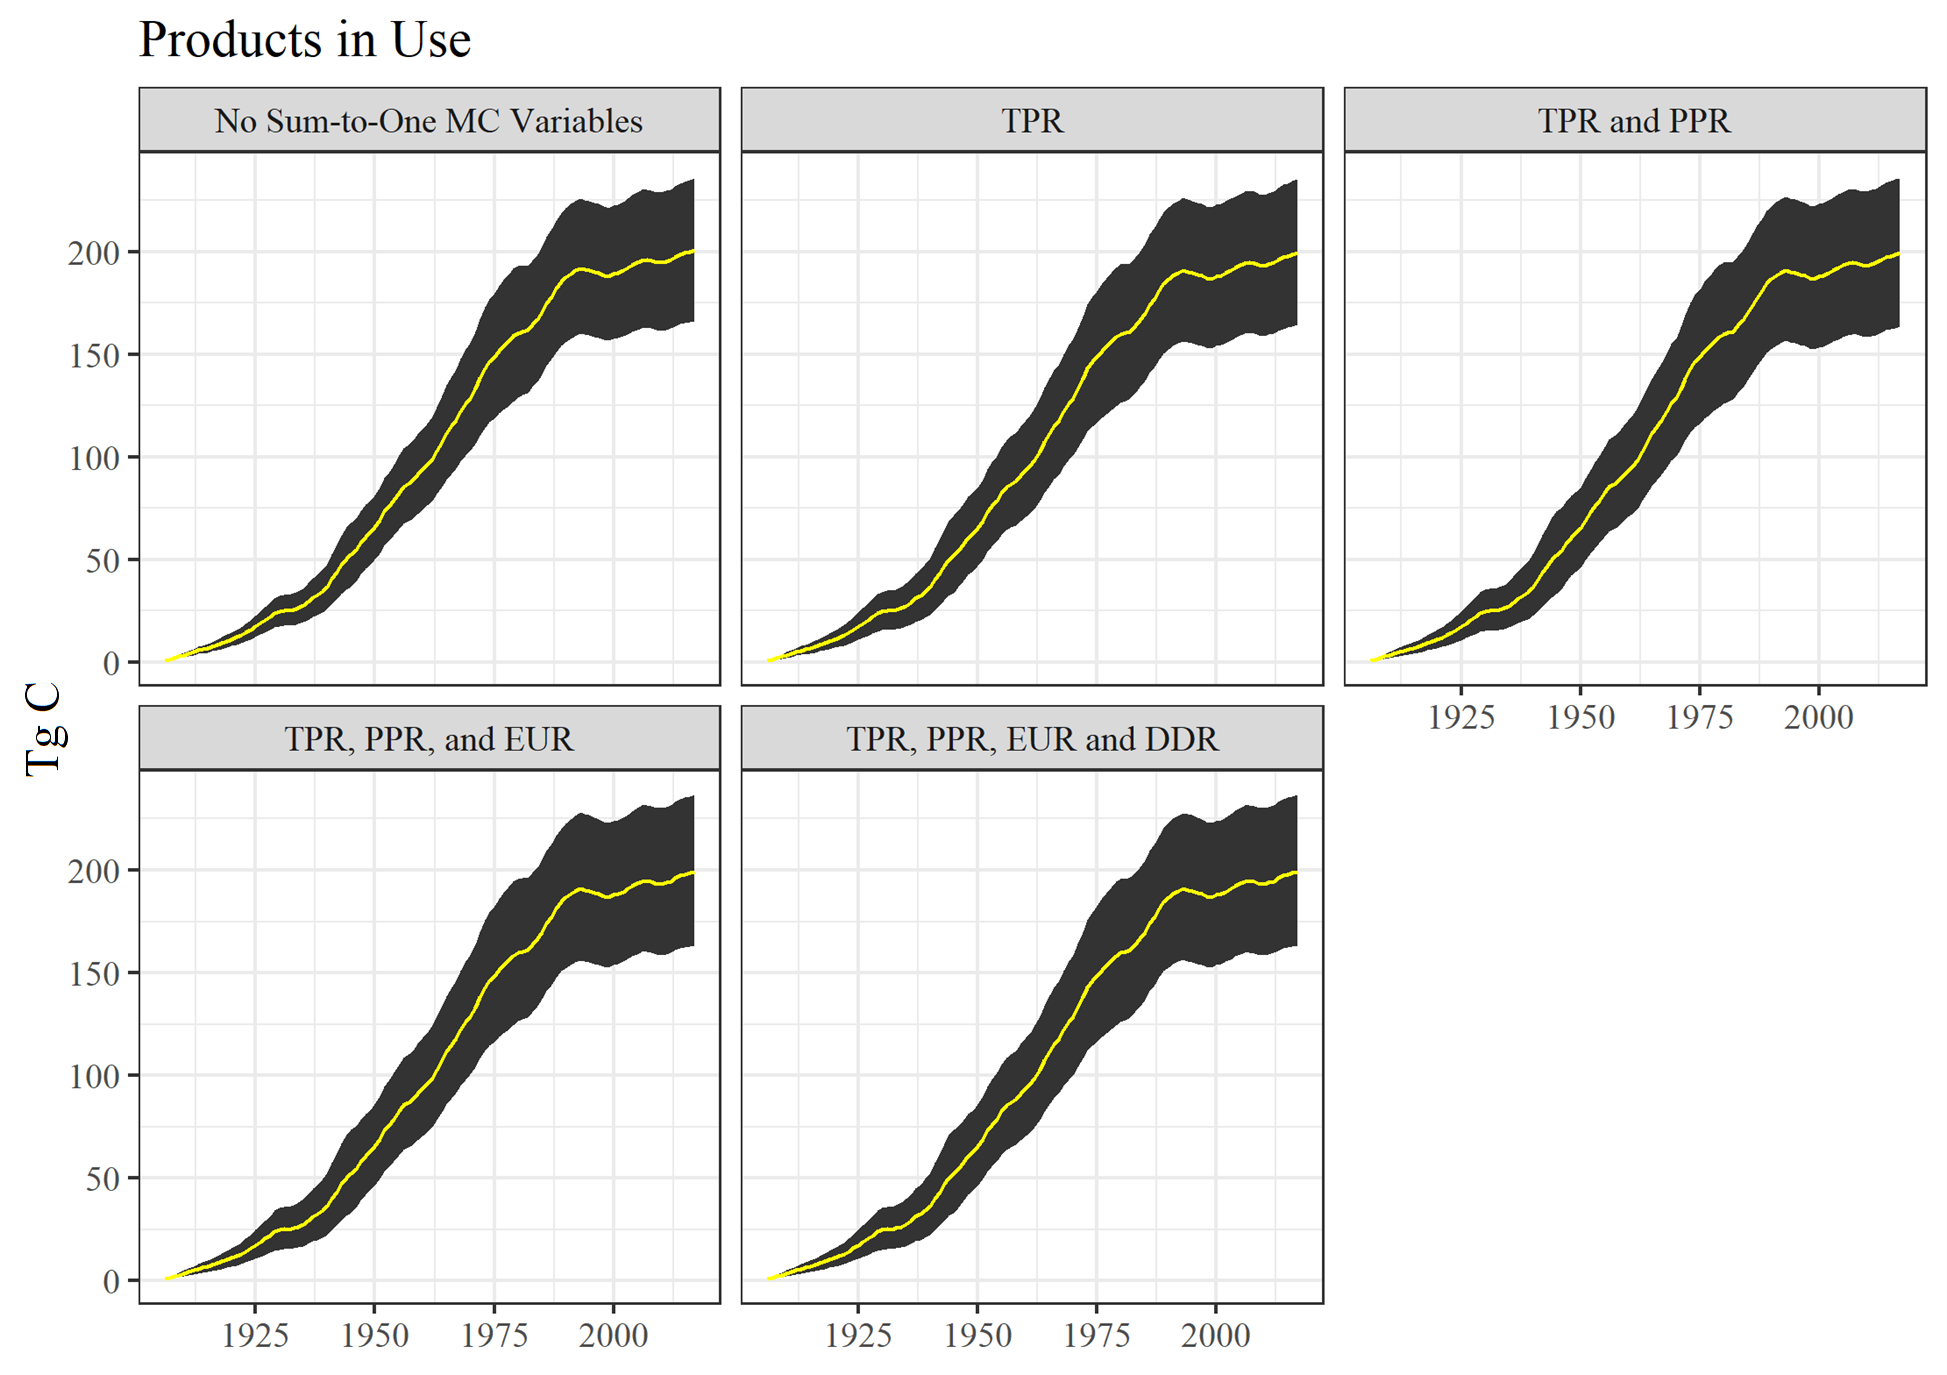
\includegraphics[width=1\linewidth]{images/MC_tests4} \caption{Monte Carlo simulation outputs for Products in Use for different Monte Carlo construction stages.  See text for acronym definitions.}\label{fig:mc-tests4-fig}
\end{figure}

\hypertarget{ft}{%
\chapter{Frequently Asked Questions and Troubleshooting}\label{ft}}

\hypertarget{ft-faqs}{%
\section{Frequently Asked Questions}\label{ft-faqs}}

\emph{Q: Why can't I access the code on the GitHub page? I'm getting a
404 error screen.}\\
A: To access the files you will need to create a GitHub account.

\emph{Q: I'm creating an input file. Do I have to have harvest ownership
data? All I have are totals.}\\
A: The model can run well without ownership data. Just have two columns
for the harvest data: Year and Total. The ownership-focused Shiny app
figures will not display data, and a few of the tables will not include
data either. Everything else should work fine.

\emph{What if I only want to view California and Oregon data and do not
want to run the tool for my own data?}\\
The Shiny app is pre-loaded with California and Oregon data. For details
about each of the app displays, take a look at Chapter @ref(app).

\emph{What are the steps to create my own input data file?}\\
Chapter @ref(own) describes how to obtain template input files and what
components of those files need to be modified so that you will have a
working input file.

\emph{What are the steps to upload my own input data file to the R Shiny
web application?}\\
See Section @ref(own-shiny) as well as the steps on the app's
\textbf{Upload Data} page.

\emph{What are the details to ensure I've set up my input data file
correctly? }\\
The quality assurance (QA) step will check your file for you. However,
the details of what to include are in Section @ref(own-prov-input) and
the specific QA checks are listed in section @ref(own-qa).

\emph{What do I need to know about running the Monte Carlo Simulation?
}\\
You will need to set the number of iterations you would like the
simulation to use (see Section @ref(own-prov-input-options)). Section
@ref(own-mc) describes other aspects of running the Monte Carlo
simulation. Details on what the simulation is doing may be found in
Section @ref(model-mc).

\emph{I only have timber harvest data in hundred cubic feet (CCF). Can I
still use these data in the model?}\\
Yes! But the model needs to think that it transformed your harvest data
into cubic feet all on its own. Here is how you fool it, using a
template file:

\begin{enumerate}
\def\labelenumi{\arabic{enumi}.}
\tightlist
\item
  Create the BFCF worksheet values. For Conversion, use the value 1.
  StartYear = your earliest data year or earlier. EndYear = your last
  harvest data year. That's right, only one row of input values.\\
\item
  Create bogus (yet usable) Harvest\_MBF worksheet values. Simply
  multiply each of your ownership and Total CCF values by 10. Place them
  in this table.\\
\item
  Everything else is the same. Fill in your TimberProdRatios and change
  any other values you need (see Chapter @ref(own)).
\end{enumerate}

\hypertarget{ft-trbl}{%
\section{Troubleshooting}\label{ft-trbl}}

\begin{enumerate}
\def\labelenumi{\arabic{enumi}.}
\tightlist
\item
  When uploading data, there can be an error message that appears in red
  right below the Browse button:\\
  \texttt{\textless{}!DOCTYPE\ HTML\textgreater{}\textless{}html\ lang=”en”\textgreater{}\textless{}head\textgreater{}}
\end{enumerate}

If this appears it is best to rebuild the excel file. There does not
appear to be a way to circumvent this issue aside from constructing a
new file (the file name is probably irrelevant so long as it does not
contain weird characters). We recommend that users cut-copy-paste from
the excel file into a blank file.

\hypertarget{refs}{}
\begin{CSLReferences}{1}{0}
\leavevmode\vadjust pre{\hypertarget{ref-adams2006}{}}%
Adams, Darius Mainard. 2006. {``Estimated Timber Harvest by US Region
and Ownership, 1950-2002.''} \emph{Gen. Tech. Rep. PNW-659. Portland,
OR: U.S. Department of Agriculture, Forest Service, Pacific Northwest
Research Station.}

\leavevmode\vadjust pre{\hypertarget{ref-anderson2013}{}}%
Anderson, Nathaniel, Jesse Young, Keith D. Stockmann, Kenneth Skog, Sean
Healey, Daniel R. Loeffler, J. Greg Jones, and James Morrison. 2013.
{``Regional and Forest-Level Estimates of Carbon Stored in Harvested
Wood Products from the United States Forest Service Northern Region,
1906-2010.''} \emph{Gen. Tech. Rep. RMRS-GTR-311. Fort Collins, CO: US
Department of Agriculture, Forest Service, Rocky Mountain Research
Station.}, 114 pp.

\leavevmode\vadjust pre{\hypertarget{ref-barlaz1998}{}}%
Barlaz, Morton A. 1998. {``Carbon Storage During Biodegradation of
Municipal Solid Waste Components in Laboratory-Scale Landfills.''}
\emph{Global Biogeochemical Cycles} 12 (2): 373--80.

\leavevmode\vadjust pre{\hypertarget{ref-barrette1970}{}}%
Barrette, Brian R., Donald R. Gedney, and Daniel D. Oswald. 1970.
\emph{California Timber Industries, 1968: Mill Characteristics and Wood
Supply}. Division of Forestry, State of California.

\leavevmode\vadjust pre{\hypertarget{ref-bolsinger1976}{}}%
Bolsinger, Charles L. 1976. \emph{Timber Resources of Northern Interior
California, 1970}. Vol. 65. US Department of Agriculture, Forest
Service, Pacific Northwest Forest; Range Experimental Station, US.

\leavevmode\vadjust pre{\hypertarget{ref-buendia2019}{}}%
Buendia, Calvo E., Kiyoto Tanabe, Andrej Kranjc, Jamsranjav Baasansuren,
Maya Fukuda, Ngarize Sekai, A. Osako, Yurii Pyrozhenko, P. Shermanau,
and Sandro Federici, eds. 2019. \emph{2019 Refinement to the 2006 IPCC
Guidelines for National Greenhouse Gas Inventories, Volume 4:
Agriculture, Forestry, and Other Land Use.} Switzerland: IPCC.

\leavevmode\vadjust pre{\hypertarget{ref-butler2014nw}{}}%
Butler, Edward, Keith D. Stockmann, Nathaniel Anderson, Ken Skog, Sean
Healey, Daniel R. Loeffler, J Greg Jones, James Morrison, and Jesse
Young. 2014. {``Estimates of Carbon Stored in Harvested Wood Products
from United States Forest Service Pacific Northwest Region,
1909-2012.''} \emph{Unpublished Report. Missoula, MT: US Department of
Agriculture, Forest Service, Rocky Mountain Research Station, Forestry
Sciences Laboratory. 28 p.}
\url{https://www.fs.usda.gov/rmrs/publications/estimates-carbon-stored-harvested-wood-products-united-states-forest-service-pacific}.

\leavevmode\vadjust pre{\hypertarget{ref-butler2014sw}{}}%
Butler, Edward, Keith D. Stockmann, Nathaniel Anderson, Jesse Young, Ken
Skog, Sean Healey, Daniel R. Loeffler, J Greg Jones, and James Morrison.
2014. {``Estimates of Carbon Stored in Harvested Wood Products from
United States Forest Service Southwestern Region, 1909-2012.''}
\emph{Unpublished Report. Missoula, MT: US Department of Agriculture,
Forest Service, Rocky Mountain Research Station, Forestry Sciences
Laboratory. 27 p.}

\leavevmode\vadjust pre{\hypertarget{ref-R-lhs}{}}%
Carnell, Rob. 2022. \emph{Lhs: Latin Hypercube Samples}.
\url{https://github.com/bertcarnell/lhs}.

\leavevmode\vadjust pre{\hypertarget{ref-R-shiny}{}}%
Chang, Winston, Joe Cheng, JJ Allaire, Carson Sievert, Barret Schloerke,
Yihui Xie, Jeff Allen, Jonathan McPherson, Alan Dipert, and Barbara
Borges. 2021. \emph{Shiny: Web Application Framework for r}.
\url{https://shiny.rstudio.com/}.

\leavevmode\vadjust pre{\hypertarget{ref-christensen2020}{}}%
Christensen, Glenn A., Andrew N. Gray, Olaf Kuegler, Nadia A. Tase, and
Mark Rosenberg. 2020. {``AB 1504 California Forest Ecosystem and
Harvested Wood Product Carbon Inventory: 2018 Reporting Period.''}
California Department of Forestry; Fire Protection.

\leavevmode\vadjust pre{\hypertarget{ref-christensen2021}{}}%
---------. 2021. {``AB 1504 California Forest Ecosystem and Harvested
Wood Product Carbon Inventory: 2019 Reporting Period.''}

\leavevmode\vadjust pre{\hypertarget{ref-eleazer1997}{}}%
Eleazer, William E., William S. Odle, Yu-Sheng Wang, and Morton A.
Barlaz. 1997. {``Biodegradability of Municipal Solid Waste Components in
Laboratory-Scale Landfills.''} \emph{Environmental Science \&
Technology} 31 (3): 911--17.

\leavevmode\vadjust pre{\hypertarget{ref-freed2004}{}}%
Freed, R. 2004. {``Open-Dump and Landfill Timeline Spreadsheet.
Unpublished.''}

\leavevmode\vadjust pre{\hypertarget{ref-freed2003}{}}%
Freed, R, and C Mintz. 2003. {``Memorandum: Revised Input Data for
WOODCARB.''}

\leavevmode\vadjust pre{\hypertarget{ref-hiserote1978}{}}%
Hiserote, Bruce A., and James O. Howard. 1978. \emph{California's Forest
Industry, 1976}. 80. Department of Agriculture, Forest Service, Pacific
Northwest Forest; Range Experimental Station, US.

\leavevmode\vadjust pre{\hypertarget{ref-howard1974}{}}%
Howard, James O. 1974. {``California Forest Industry: Wood Consumption
and Characteristics, 1972. Forest Service Resource Bulletin.''} Forest
Service, Portland, OR (USA). Pacific Northwest Forest; Range
Experimental Station, US.

\leavevmode\vadjust pre{\hypertarget{ref-ipcc2014}{}}%
IPCC. 2014. Edited by Taka Hiraishi, Thema Krug, Kiyoto Tanabe, Nalin
Srivastava, Jamsranjav Baasansuren, Maya Fukuda, and Tiffany Troxler.
Switzerland: Intergovernmental Panel on Climate Change: IPCC,
Switzerland.
\url{http://www.ipcc-nggip.iges.or.jp/public/kpsg/pdf/KP_Supplement_Entire_Report.pdf}.

\leavevmode\vadjust pre{\hypertarget{ref-keegan2010}{}}%
Keegan, Charles E. III, Todd A. Morgan, Keith A. Blatner, and Jean M.
Daniels. 2010. {``Trends in Lumber Processing in the Western United
States. Part i: Board Foot Scribner Volume Per Cubic Foot of Timber.''}
\emph{Forest Products Journal} 60 (2): 133--39.

\leavevmode\vadjust pre{\hypertarget{ref-loeffler2019}{}}%
Loeffler, Daniel R., Nathaniel Anderson, Keith D. Stockmann, Todd A.
Morgan, and Nadia A. Tase. 2019. {``Harvested Wood Products Carbon
Chapters 5 and 6.''} In \emph{AB 1504 California Forest Ecosystem and
Harvested Wood Product Carbon Inventory: 2017 Reporting Period. Final
Report.}, 102--37. Sacramento, CA: California Department of Forestry;
Fire Protection; California Board of Forestry; Fire Protection.: U.S.
Forest Service agreement no. 18-CO-11052021-214, 17-CO-11261979-086,
California Department of Forestry; Fire Protection agreement no.
8CA04056; 8CA03714; the University of Montana.
\url{https://bof.fire.ca.gov/media/8026/4-final_1504_forest_ecosys_hwp_c_2017_13feb19_full.pdf}.

\leavevmode\vadjust pre{\hypertarget{ref-loeffler2014er}{}}%
Loeffler, Daniel R., Nathaniel Anderson, Keith D. Stockmann, Ken Skog,
Sean Healey, J Greg Jones, James Morrison, and Jesse Young. 2014a.
{``Estimates of Carbon Stored in Harvested Wood Products from United
States Forest Service Eastern Region, 1911-2012.''} \emph{Unpublished
Report. Missoula, MT: US Department of Agriculture, Forest Service,
Rocky Mountain Research Station, Forestry Sciences Laboratory. 27 p.}

\leavevmode\vadjust pre{\hypertarget{ref-loeffler2014sr}{}}%
Loeffler, Daniel R., Nathaniel Anderson, Keith D. Stockmann, Ken Skog,
Sean Healey, J. Greg Jones, James Morrison, and Jesse Young. 2014b.
{``Estimates of Carbon Stored in Harvested Wood Products from United
States Forest Service Southern Region, 1911-2012.''} \emph{Unpublished
Report. Missoula, MT: US Department of Agriculture, Forest Service,
Rocky Mountain Research Station, Forestry Sciences Laboratory. 27 p.}
\url{https://www.fs.usda.gov/rmrs/publications/estimates-carbon-stored-harvested-wood-products-united-states-forest-service-pacific}.

\leavevmode\vadjust pre{\hypertarget{ref-lucey202X}{}}%
Lucey, Taylor, Nadia A. Tase, N. Prakash, R. Bergman, D. Nichols, Andrew
N. Gray, K. Poonam, and K. Sahoo. In review. {``Chapter 3: Harvested
Wood Product Model Synthesis.''} In \emph{Management and Policy Effects
on Forest Sector Carbon: A Synthesis of Model Approaches to Guide
Projections on the West Coast. General Technical Report PNW-GTR-Xxx},
edited by Andrew N. Gray and Taylor Lucey, xxx--. Portland, OR: USDA
Forest Service Pacific Northwest Research Station.

\leavevmode\vadjust pre{\hypertarget{ref-marcille2020}{}}%
Marcille, Kate C., Todd A. Morgan, Chelsea P. McIver, and Glenn A.
Christensen. 2020. {``California's Forest Products Industry and Timber
Harvest, 2016.''} \emph{Gen. Tech. Rep. PNW-GTR-994. Portland, OR: US
Department of Agriculture, Forest Service, Pacific Northwest Research
Station. 58 p.} 994.

\leavevmode\vadjust pre{\hypertarget{ref-mciver2015}{}}%
McIver, Chelsea P., Joshua P. Meek, Micah G. Scudder, Colin B Sorenson,
Todd A. Morgan, and Glenn A. Christensen. 2015. {``California's Forest
Products Industry and Timber Harvest, 2012.''} \emph{Gen. Tech. Rep.
PNW-GTR-908. Portland, OR: US Department of Agriculture, Forest Service,
Pacific Northwest Research Station. 49 p.} 908.

\leavevmode\vadjust pre{\hypertarget{ref-mckeever2009}{}}%
McKeever, David B. 2009. {``Estimated Annual Timber Products Consumption
in Major End Uses in the United States, 1950-2006.''} \emph{General
Technical Report FPL-GTR-181} 181: 1--47.

\leavevmode\vadjust pre{\hypertarget{ref-mckeever2011}{}}%
McKeever, David B., and James L. Howard. 2011. {``Solid Wood Timber
Products Consumption in Major End Uses in the United States, 1950-2009:
A Technical Document Supporting the Forest Service 2010 RPA
Assessment.''} \emph{General Technical Report FPL-GTR-199. Madison, WI:
US Dept. Of Agriculture, Forest Service, Forest Products Laboratory,
2011: 39 p.} 199.

\leavevmode\vadjust pre{\hypertarget{ref-melosi1982}{}}%
Melosi, Martin V. 1982. {``Garbage in the Cities: Refuse, Reform, and
the Environment, 1880-1980.''} \emph{Texas A \& M Univ. Press, College
Station, TX 77843. 1982.}

\leavevmode\vadjust pre{\hypertarget{ref-melosi1999}{}}%
---------. 1999. \emph{The Sanitary City}. Johns Hopkins Univ. Press,
Baltimore, MD.

\leavevmode\vadjust pre{\hypertarget{ref-morgan2004}{}}%
Morgan, Todd A. 2004. \emph{California's Forest Products Industry: A
Descriptive Analysis}. Vol. 615. US Department of Agriculture, Pacific
Northwest Research Station.

\leavevmode\vadjust pre{\hypertarget{ref-morgan2012}{}}%
Morgan, Todd A., Jason P. Brandt, Kathleen E. Songster, Charles E.
Keegan, and Glenn A. Christensen. 2012. {``California's Forest Products
Industry and Timber Harvest, 2006.''} \emph{Gen. Tech. Rep. PNW-GTR-866.
Portland, OR: US Department of Agriculture, Forest Service, Pacific
Northwest Research Station. 48 p} 866.

\leavevmode\vadjust pre{\hypertarget{ref-morgan2021}{}}%
Morgan, Todd A., Thomas S. Donahue, Thale Dillon, Andrew Yost, and
Jeremiah D. Groom. 2021. {``Oregon Harvested Wood Products Carbon
Inventory, 1906-2018.''} \emph{Report Completed Through Agreement No.
18-CO-11261979-074 Between the U.S. Forest Service, Pacific Northwest
Research Station and the Oregon Department of Forestry; and Agreement
No. 18-CR-11261979-095 Between the U.S. Forest Service, Pacific
Northwest Research Station and the University of Montana, Bureau of
Business and Economic Research.}, 56 p.
\url{https://www.oregon.gov/odf/forestbenefits/Documents/oregon-harvested-wood-products-carbon-inventory-report.pdf}.

\leavevmode\vadjust pre{\hypertarget{ref-nichols2020}{}}%
Nichols, Michael C., Todd A. Morgan, Glenn A. Christensen, and Nadia A.
Tase. 2020. {``Estimated Carbon Stored in Harvested Wood Products in
Washington, USA: 1906 -- 2018, Draft Report.''} \emph{Prepared for the
Washington Department of Natural Resources. Olympia, Washington.}, 30 p.
\url{https://www.dnr.wa.gov/publications/em_wa_carbon_121420.pdf}.

\leavevmode\vadjust pre{\hypertarget{ref-penman2000}{}}%
Penman, James, Dina Kruger, Ian Galbally, Taka Hiraishi, Buruhani
Nyenzi, S. Emmanul, L. Buendia, et al. 2000. \emph{Good Practice
Guidance and Uncertainty Management in National Greenhouse Gas
Inventories: IPCC National Greenhouse Gas Inventories Programme}.
Institute for Global Environmental Strategies, Japan.

\leavevmode\vadjust pre{\hypertarget{ref-pingoud2006}{}}%
Pingoud, Kim, Kenneth E. Skog, Daniel L. Martino, Mario Tonosaki, and
Zhang Xiaoquan. 2006. {``Harvested Wood Products.''} In \emph{2006 IPCC
Guidelines for National Greenhouse Gas Inventories}, edited by H. Simon.
Eggleston, L. Buendia, Kyoko Miwa, Todd Ngara, and Kiyoto Tanabe. Japan:
IGES.

\leavevmode\vadjust pre{\hypertarget{ref-R-base}{}}%
R Core Team. 2021. \emph{R: A Language and Environment for Statistical
Computing}. Vienna, Austria: R Foundation for Statistical Computing.
\url{https://www.R-project.org/}.

\leavevmode\vadjust pre{\hypertarget{ref-row1996}{}}%
Row, Clark, and R. B. Phelps. 1996. {``Wood Carbon Flows and Storage
After Timber Harvest.''} \emph{Forests and Global Change} 2: 27--58.

\leavevmode\vadjust pre{\hypertarget{ref-ruter2019}{}}%
Rüter, Sebastian, R. W. Matthews, Mattias Lundblad, Atsushi Sato, and R.
Hassan. 2019. {``Chapter 12: Harvested Wood Products.''} In \emph{2019
Refinement to the 2006 IPCC Guidelines for National Greenhouse Gas
Inventories, Volume 4: Agriculture, Forestry, and Other Land Use.},
edited by Calvo E. Buendia, Kiyoto Tanabe, Andrej Kranjc, Jamsranjav
Baasansuren, Maya Fukuda, Ngarize Sekai, A. Osako, Yurii Pyrozhenko, P.
Shermanau, and Sandro Federici. Switzerland: IPCC.

\leavevmode\vadjust pre{\hypertarget{ref-skog2008}{}}%
Skog, Kenneth E. 2008. {``Sequestration of Carbon in Harvested Wood
Products for the United States.''} \emph{Forest Products Journal. Vol.
58, No. 6 (June 2008): Pages 56-72}.

\leavevmode\vadjust pre{\hypertarget{ref-skog1998}{}}%
Skog, Kenneth E., and Geraldine A. Nicholson. 1998. {``Carbon Cycling
Through Wood Products: The Role of Wood and Paper Products in Carbon
Sequestration.''} \emph{Forest Products Journal} 48 (7): 75--83.

\leavevmode\vadjust pre{\hypertarget{ref-skog2000}{}}%
---------. 2000. {``Carbon Sequestration in Wood and Paper Products.''}
\emph{In: Joyce, Linda A.; Birdsey, Richard A., Technical Editors. 2000.
The Impact of Climate Change on America's Forests: A Technical Document
Supporting the 2000 USDA Forest Service RPA Assessment. Gen. Tech. Rep.
RMRS-GTR-59. Fort Collins, CO: US Department of Agriculture, Forest
Service, Rocky Mountain Research Station. P. 79-88} 59.

\leavevmode\vadjust pre{\hypertarget{ref-smith2006}{}}%
Smith, James E., Linda S. Heath, Kenneth E. Skog, and Richard A.
Birdsey. 2006. {``Methods for Calculating Forest Ecosystem and Harvested
Carbon with Standard Estimates for Forest Types of the United States.''}
\emph{Gen. Tech. Rep. NE-343. Newtown Square, PA: United States
Department of Agriculture, Forest Service, Northeastern Research
Station} 343.

\leavevmode\vadjust pre{\hypertarget{ref-stockmann2012}{}}%
Stockmann, Keith D., Nathaniel M. Anderson, Kenneth E. Skog, Sean P.
Healey, Daniel R. Loeffler, Greg Jones, and James F. Morrison. 2012.
{``Estimates of Carbon Stored in Harvested Wood Products from the United
States Forest Service Northern Region, 1906-2010.''} \emph{Carbon
Balance and Management} 7 (1): 1--16.

\leavevmode\vadjust pre{\hypertarget{ref-stockmann2014nr}{}}%
Stockmann, Keith D., Nathaniel Anderson, Jesse Young, Ken Skog, Sean
Healey, Daniel R. Loeffler, Edward Butler, J Greg Jones, and James
Morrison. 2014a. {``Estimates of Carbon Stored in Harvested Wood
Products from United States Forest Service Northern Region,
1906-2012.''} \emph{Unpublished Report. Missoula, MT: US Department of
Agriculture, Forest Service, Rocky Mountain Research Station, Forestry
Sciences Laboratory. 27 p.}

\leavevmode\vadjust pre{\hypertarget{ref-stockmann2014rmr}{}}%
---------. 2014b. {``Estimates of Carbon Stored in Harvested Wood
Products from United States Forest Service Rocky Mountain Region,
1906-2012.''} \emph{Unpublished Report. Missoula, MT: US Department of
Agriculture, Forest Service, Rocky Mountain Research Station, Forestry
Sciences Laboratory. 27 p.}

\leavevmode\vadjust pre{\hypertarget{ref-stockmann2014imr}{}}%
Stockmann, Keith D., Nathaniel Anderson, Jesse Young, Ken Skog, Sean
Healey, Daniel R. Loeffler, Edward Butler, J. Greg Jones, and James
Morrison. 2014c. {``Estimates of Carbon Stored in Harvested Wood
Products from United States Forest Service Intermountain Region,
1911-2012.''} \emph{Unpublished Report. Missoula, MT: US Department of
Agriculture, Forest Service, Rocky Mountain Research Station, Forestry
Sciences Laboratory. 28 p.}

\leavevmode\vadjust pre{\hypertarget{ref-epa2006}{}}%
US EPA. 2006. {``Municipal Solid Waste in the United States: 2000 Facts
and Figures.''} \emph{Epa530-R-06-011. Office of Solid Waste and
Emergency Response (5306p), Washington D.C.}

\leavevmode\vadjust pre{\hypertarget{ref-usepa2020}{}}%
---------. 2020. {``Waste Reduction Model (WARM).''} \emph{US
Environmental Protection Agency, Washington, DC}.
\url{https://www.epa.gov/warm/versions-waste-reduction-model-warm\#15}.

\leavevmode\vadjust pre{\hypertarget{ref-R-renv}{}}%
Ushey, Kevin. 2022. \emph{Renv: Project Environments}.
\url{https://rstudio.github.io/renv/}.

\leavevmode\vadjust pre{\hypertarget{ref-ward1995}{}}%
Ward, Franklin R. 1995. \emph{California's Forest Products Industry,
1992. Res. Bull. PNW-RB-206}. US Department of Agriculture, Forest
Service, Pacific Northwest Research Station.

\leavevmode\vadjust pre{\hypertarget{ref-ward1997}{}}%
---------. 1997. \emph{California's Forest Products Industry, 1994. Res.
Bull. PNW-RB-217}. US Department of Agriculture, Forest Service, Pacific
Northwest Research Station.

\leavevmode\vadjust pre{\hypertarget{ref-warren2005}{}}%
Warren, Debra D. 2005. \emph{Production, Prices, Employment, and Trade
in Northwest Forest Industries, All Quarters 2003}. DIANE Publishing.

\leavevmode\vadjust pre{\hypertarget{ref-wickham2021}{}}%
Wickham, Hadley. 2021. \emph{Mastering Shiny}. " O'Reilly Media, Inc.".

\end{CSLReferences}

\backmatter
\end{document}
